\documentclass[lang=cn,a4paper,11pt,openany,twoside]{elegantbook}

\let\arrowvert\relax
%\usepackage{unicode-math}

\let\arrowvert\relax


\usepackage{xeCJK}
\usepackage{amsmath} % 建议
\usepackage{amssymb} % 可选，提供更多符号

\usepackage{ctex}
\let\openbox\relax

\usepackage{tikz}
\usetikzlibrary{decorations.pathreplacing,arrows.meta}

%调整页边距
\usepackage{geometry}
\geometry{top=2cm, bottom=2.25cm, outer=2cm, inner=2.5cm}


\usepackage{setspace}
\setstretch{1.3}

%设定行间距
\usepackage{calc}
\setlength{\lineskip}{\baselineskip-\ccwd}
\setlength{\lineskiplimit}{2.5pt}



%浮动图片
\usepackage{wrapfig}
%图标表格注记
\usepackage{caption}
%圆圈数字
\usepackage{pifont}
%表格换行
\usepackage{makecell}
%表格颜色
\usepackage[table]{xcolor}
\colorlet{rowcolcolor}{structurecolor!25!white}

%行间距加大
\newcommand{\wideline}{\setlength{\lineskip}{\baselineskip-\ccwd}\setlength{\lineskiplimit}{2.5pt}}
%蓝色加粗
\definecolor{titleblue}{HTML}{3498DB}
\newcommand{\bluebf}[1]{\textcolor{structurecolor}{\textbf{#1}}}


%向量
\usepackage[f]{esvect}

\renewcommand{\vector}[1]{\vv{#1}}
%平面
\newcommand{\plane}{\text{平面}\ }
%平行且等于
\newcommand{\paraleq}{%
    \mathrel{\text{%
        \tikz[baseline]
        \draw (.1em,0ex) -- (.9em,0ex)
        (.1em,-.425ex) -- (.9em,-.425ex)
        (.350em,.1ex) -- (.650em,1.5ex)
        (.550em,.1ex) -- (.850em,1.5ex);}}}

\newcommand{\mb}{\mathbb}
\newcommand{\z}{\text}
\renewcommand{\a}{\alpha}
\renewcommand{\b}{\beta}
\renewcommand{\d}{\mathrm{d}}
\newcommand{\D}{\Delta}
\renewcommand{\l}{\lambda}
\newcommand{\m}{\mu}
\newcommand{\fl}{\fillin}
\newcommand{\pr}{\paren}
\newcommand{\p}{\uppi}
\renewcommand{\th}{\theta}
\newcommand{\lam}{\lambda}
\newcommand{\rttri}{\mathrm{Rt}\triangle}
\newcommand{\npar}{\par\noindent}
\DeclareSymbolFont{ugmL}{OMX}{mdugm}{m}{n}
\DeclareMathAccent{\wideparen}{\mathord}{ugmL}{"F3}
\newcommand{\sigmaalg}{\sigma-\text{代数}}
\newcommand{\setjot}[1][0]{\setlength{\jot}{#1 pt}}


%填空题下划线
\newcommand{\fillin}[1][3.5]{%
  \nolinebreak % 不在此处断行
  \hspace{0.2em}%
  \rule[-0.5ex]{#1em}{0.5pt}% 轻微下沉模拟“下划线”效果
  \hspace{0.05em}
}

%调整环境内图片环绕
\usepackage{mwe}
\newcommand{\wrapfix}[1][-1]{\begin{wrapfigure}{r}{0.001\textwidth}%
    \vspace{#1 em}%
    \includegraphics[width=0.001\textwidth]{example-image}%
    \end{wrapfigure}}



%分式使用行间版
\everymath{\displaystyle}


\usepackage{myenvironment}


%elegantbook部分修改
\usepackage{elegantfix}

\usepackage{tcolorbox}

\usepackage{xcolor}
\definecolor{mygray}{RGB}{240,240,240}
\tcbset{
  colback=mygray,
  boxrule=0pt,
}
\graphicspath{ {./fig/} }
\newcommand{\HRule}{\begin{center}\rule{0.9\linewidth}{0.2mm}\end{center}}
\newcommand{\customfootnote}[1]{
  \let\thefootnote\relax\footnotetext{#1}
}

%强制右页开始
\makeatletter
\newcommand{\ForceRightPage}{%
  \clearpage
  \ifodd\value{page}\relax
    % 已经是奇数页，什么也不做
  \else
    \hbox{}\thispagestyle{empty}\newpage
  \fi
}
\makeatother


\raggedbottom


\begin{document}


\title{Notes for Differential Geometry}
\date{}
\maketitle
\setcounter{page}{1}

\frontmatter
\pagenumbering{roman}     % 目录等用罗马数字
\clearpage
\tableofcontents
\clearpage

\ForceRightPage
\mainmatter

\section*{Section 1 Parameterized curves}

\begin{tcolorbox}
\section*{第1节 参数曲线}
\end{tcolorbox}

There are two ways to view a curve. Imagine you register for a mountain bike race. The race track, as marked by the organizers, exists independently of you and is described by a certain set of points in space. This one-dimensional object is what we call a curve. However, as a participant in the race, you experience the curve differently: you move along it, and your position can be recorded at different times. This function, which maps time to your position in space, is what we refer to as a parameterized curve.

\begin{tcolorbox}
观察一条曲线有两种方式。想象你报名参加一场山地自行车比赛。比赛路线由组织者标记，独立于你存在，并由空间中的一组点描述。这一维对象我们称为曲线。然而，作为比赛的参与者，你对曲线的体验不同:你沿着它移动，你的位置可以在不同时间被记录。这一函数，将时间映射到你在空间中的位置，我们称之为参数化曲线。
\end{tcolorbox}

\HRule

Definition 1

\begin{tcolorbox}
定义1
\end{tcolorbox}

(Curve)

\begin{tcolorbox}
(曲线)
\end{tcolorbox}

\HRule

A parameterized curve is a smooth map \(c : I \rightarrow  {\mathbb{R}}^{n}\left( {n = 2,3}\right)\) , where \(I\) is an interval, usually \(\left\lbrack  {a,b}\right\rbrack\) or(0,1). A curve is the image of a parameterized curve, i.e., the set \(\{ c\left( t\right)  : t \in  I\}\) .

\begin{tcolorbox}
参数化曲线是一个光滑映射 \(c : I \rightarrow  {\mathbb{R}}^{n}\left( {n = 2,3}\right)\) ，其中 \(I\) 是一个区间，通常为 \(\left\lbrack  {a,b}\right\rbrack\) 或(0,1)。一条曲线是参数化曲线的像，即集合 \(\{ c\left( t\right)  : t \in  I\}\) 。
\end{tcolorbox}

Note that the parameter \(t\) does not necessarily represent time; it can be any parameter that varies along the curve. For example, in the case of the bike race, \(t\) could represent the distance traveled along the track instead of the time elapsed. Nonetheless, it is often convenient to think of \(t\) as time, as it provides an intuitive way to understand the motion along the curve. In this spirit, we refer to \(\dot{c}\left( t\right)  = \frac{\mathrm{d}c}{\mathrm{\;d}t}\) as the velocity vector and \(\ddot{c}\left( t\right)  = \frac{\mathrm{d}\dot{c}}{\mathrm{\;d}t}\) as the acceleration vector.

\begin{tcolorbox}
注意，参数 \(t\) 不一定代表时间；它可以是沿曲线变化的任何参数。例如，在自行车比赛中， \(t\) 可以代表沿路线行驶的距离，而非经过的时间。尽管如此，将 \(t\) 视为时间通常更方便，因为它提供了一种直观理解沿曲线运动的方式。在这种思想下，我们将 \(\dot{c}\left( t\right)  = \frac{\mathrm{d}c}{\mathrm{\;d}t}\) 称为速度向量，将 \(\ddot{c}\left( t\right)  = \frac{\mathrm{d}\dot{c}}{\mathrm{\;d}t}\) 称为加速度向量。
\end{tcolorbox}

There are many different parameterizations for the same curve. For example, different riders may travel at different speeds, leading to different parameterizations of the same physical curve. So we need a way to pass from one parameterization to another.

\begin{tcolorbox}
对于同一条曲线，有许多不同的参数化方式。例如，不同的骑手可能以不同的速度行驶，导致同一物理曲线的不同参数化。因此，我们需要一种方法，将一种参数化转换为另一种参数化。
\end{tcolorbox}

\HRule

Definition 2 (Diffeomorphism)

\begin{tcolorbox}
定义2(微分同胚)
\end{tcolorbox}

\HRule

A smooth map \(\varphi  : {I}_{2} \rightarrow  {I}_{1}\) is called a diffeomorphism if \(\varphi\) is bijective (one-to-one and onto) and its inverse \({\varphi }^{-1}\) is also smooth.

\begin{tcolorbox}
如果光滑映射 \(\varphi  : {I}_{2} \rightarrow  {I}_{1}\) 是双射(既单射又满射)，且其逆映射 \({\varphi }^{-1}\) 也是光滑的，则称 \(\varphi  : {I}_{2} \rightarrow  {I}_{1}\) 为微分同胚。
\end{tcolorbox}

\HRule

Definition 3

\begin{tcolorbox}
定义3
\end{tcolorbox}

(Reparameter-ization)

\begin{tcolorbox}
(重新参数化)
\end{tcolorbox}

\HRule

If \(\varphi  : {I}_{2} \rightarrow  {I}_{1}\) is a diffeomorphism with \({}^{a}{\varphi }^{\prime }\left( t\right)  > 0\) and \({c}_{1} : {I}_{1} \rightarrow  {\mathbb{R}}^{n}\) is a parameterized curve, then \({c}_{2}\left( t\right)  = {c}_{1}\left( {\varphi \left( t\right) }\right)  : {I}_{2} \rightarrow  {\mathbb{R}}^{n}\) is also a parameterized curve, called the reparameterization of \({c}_{1}\) by \(\varphi\) .

\begin{tcolorbox}
如果 \(\varphi  : {I}_{2} \rightarrow  {I}_{1}\) 是一个具有 \({}^{a}{\varphi }^{\prime }\left( t\right)  > 0\) 和 \({c}_{1} : {I}_{1} \rightarrow  {\mathbb{R}}^{n}\) 的微分同胚，且 \({c}_{2}\left( t\right)  = {c}_{1}\left( {\varphi \left( t\right) }\right)  : {I}_{2} \rightarrow  {\mathbb{R}}^{n}\) 是一个参数化曲线，则 \({c}_{1}\) 的重新参数化由 \(\varphi\) 定义，也是一条参数化曲线，称为 \({c}_{1}\) 通过 \(\varphi\) 的重新参数化。
\end{tcolorbox}

\({}^{a}\) A diffeomorphism \(\varphi\) always has either \({\varphi }^{\prime }\left( t\right)  > 0\) or \({\varphi }^{\prime }\left( t\right)  < 0\) for all \(t\) . The latter case would correspond to reversing the direction of the curve.

\begin{tcolorbox}
\({}^{a}\) 一个微分同胚 \(\varphi\) 总是对所有 \(t\) 具有 \({\varphi }^{\prime }\left( t\right)  > 0\) 或 \({\varphi }^{\prime }\left( t\right)  < 0\) 。后者的情况对应于反转曲线的方向。
\end{tcolorbox}

We will often introduce a certain property of the curve using a parameterization, and then show that this property does not depend on the choice of parameterization. For example, the length of a curve is a property that should be independent of how we parameterize it - all riders should better agree on the length of the track, regardless of their speed.

\begin{tcolorbox}
我们经常会用参数化引入曲线的某些性质，然后证明这些性质不依赖于参数化的选择。例如，曲线的长度是一个应当与参数化方式无关的性质——所有骑手都应对轨道的长度达成一致，而不管他们的速度如何。
\end{tcolorbox}

\HRule

Definition 4 (Length of a curve)

\begin{tcolorbox}
定义4(曲线的长度)
\end{tcolorbox}

\HRule

The length of a parameterized curve \(c : I \rightarrow  {\mathbb{R}}^{n}\) is defined as

\begin{tcolorbox}
参数化曲线 \(c : I \rightarrow  {\mathbb{R}}^{n}\) 的长度定义为
\end{tcolorbox}

\[
L\left( c\right)  \mathrel{\text{ := }} {\int }_{a}^{b}\parallel \dot{c}\left( t\right) \parallel \mathrm{d}t \tag{1.1}
\]

where \(I = \left\lbrack  {a,b}\right\rbrack\) or(a, b).

\begin{tcolorbox}
其中 \(I = \left\lbrack  {a,b}\right\rbrack\) 或(a, b)。
\end{tcolorbox}

Lemma 1 | If \({c}_{2}\) is a reparameterization of \({c}_{1}\) , then the length of \({c}_{1}\) and \({c}_{2}\) are the same.

\begin{tcolorbox}
引理1 | 如果 \({c}_{2}\) 是 \({c}_{1}\) 的重新参数化，那么 \({c}_{1}\) 和 \({c}_{2}\) 的长度相同。
\end{tcolorbox}

Proof Since \({c}_{2}\left( t\right)  = {c}_{1}\left( {\varphi \left( t\right) }\right)\) for some diffeomorphism \(\varphi  : {I}_{2} \rightarrow  {I}_{1}\) , we have by the chain rule

\begin{tcolorbox}
证明:由于 \({c}_{2}\left( t\right)  = {c}_{1}\left( {\varphi \left( t\right) }\right)\) 是某个微分同胚 \(\varphi  : {I}_{2} \rightarrow  {I}_{1}\) 的参数化，我们根据链式法则得出
\end{tcolorbox}

\[
{\left. \frac{\mathrm{d}}{\mathrm{d}t}\right| }_{t}{c}_{2} = {\left. {\varphi }^{\prime }\left( t\right) \frac{\mathrm{d}}{\mathrm{d}s}\right| }_{\varphi \left( t\right) }{c}_{1}.
\]

Assume, without loss of generality, that \({I}_{1} = \left\lbrack  {{a}_{1},{b}_{1}}\right\rbrack\) and \({I}_{2} = \left\lbrack  {{a}_{2},{b}_{2}}\right\rbrack\) with \(\varphi \left( {a}_{2}\right)  = {a}_{1}\) and \(\varphi \left( {b}_{2}\right)  = {b}_{1}\) . Thus,

\begin{tcolorbox}
假设，毫无损失地， \({I}_{1} = \left\lbrack  {{a}_{1},{b}_{1}}\right\rbrack\) 和 \({I}_{2} = \left\lbrack  {{a}_{2},{b}_{2}}\right\rbrack\) 具有 \(\varphi \left( {a}_{2}\right)  = {a}_{1}\) 和 \(\varphi \left( {b}_{2}\right)  = {b}_{1}\) 。因此，
\end{tcolorbox}

\[
L\left( {c}_{2}\right)  = {\int }_{{a}_{2}}^{{b}_{2}}\begin{Vmatrix}{{\left. \frac{\mathrm{d}}{\mathrm{d}t}\right| }_{t}{c}_{2}}\end{Vmatrix}\mathrm{d}t
\]

\[
= {\int }_{{a}_{2}}^{{b}_{2}}\left| {{\varphi }^{\prime }\left( t\right) }\right|  \cdot  \begin{Vmatrix}{{\left. \frac{\mathrm{d}}{\mathrm{d}s}\right| }_{\varphi \left( t\right) }{c}_{1}}\end{Vmatrix}\mathrm{d}t
\]

\[
s = \underline{\underline{\varphi }}\left( t\right) {\int }_{{a}_{1}}^{{b}_{1}}{\begin{Vmatrix}{\left. \frac{\mathrm{d}}{\mathrm{d}s}\right| }_{s}{c}_{1}\end{Vmatrix}}_{a}{ds}
\]

\[
= L\left( {c}_{1}\right) ,
\]

where we used the reparameterization theorem for integrals in the third step.

\begin{tcolorbox}
在第三步中，我们使用了积分的重新参数化定理。
\end{tcolorbox}

The proof exhibits a general strategy that we will use often in this course: when we want to investigate a certain property of a curve or surface, we will use a parameterization to boil it down to a problem in calculus that we know how to solve. Here, we just used the chain rule and the reparameterization theorem for integrals.

\begin{tcolorbox}
该证明展示了一种我们在本课程中经常使用的通用策略:当我们想要研究某条曲线或曲面的某个性质时，我们会利用参数化将其简化为我们知道如何解决的微积分问题。在这里，我们只用了链式法则和积分的重新参数化定理。
\end{tcolorbox}

At this point, a word of caution is in order. In the definition of a curve, we required the parameterization to be smooth (i.e, all derivatives exist and are continuous). However, this does not imply that the curve itself is smooth in a geometric sense. For example, the parameterization \(c\left( t\right)  = \left( {{t}^{3},{t}^{2}}\right)\) is smooth, but the curve it describes has a cusp at the origin.

\begin{tcolorbox}
此时，需要提醒一句。在曲线的定义中，我们要求参数化是光滑的(即所有导数存在且连续)。然而，这并不意味着曲线本身在几何意义上是光滑的。例如，参数化 \(c\left( t\right)  = \left( {{t}^{3},{t}^{2}}\right)\) 是光滑的，但它所描述的曲线在原点处有一个尖点(cusp)。
\end{tcolorbox}

\begin{center}
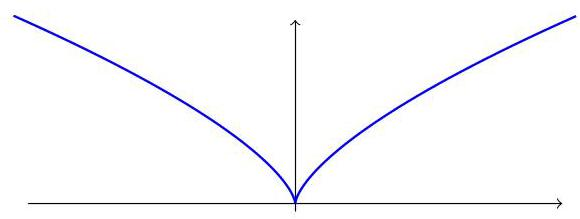
\includegraphics[width=0.4\textwidth]{fig/bo_d3cgcuc601uc738c0ulg_1_462_1366_580_219_0.jpg}
\end{center}
\hspace*{3em} 

Figure 1. Plot of the smooth curve \(c\left( t\right)  = \left( {{t}^{3},{t}^{2}}\right)\) showing a cusp at the origin.

\begin{tcolorbox}
图1。光滑曲线 \(c\left( t\right)  = \left( {{t}^{3},{t}^{2}}\right)\) 的绘图，显示在原点处有一个尖点。
\end{tcolorbox}

To avoid such singularities, we introduce the following definition.

\begin{tcolorbox}
为了避免此类奇异点，我们引入以下定义。
\end{tcolorbox}

\HRule

Definition 5

\begin{tcolorbox}
定义5
\end{tcolorbox}

(Regular curve)

\begin{tcolorbox}
(正则曲线)
\end{tcolorbox}

\HRule

A parameterized curve \(c\) is called regular if \(\dot{c}\left( t\right)  \neq  0\) for all \(t \in  I\) . Such a curve, in particular, has no cusps or corners.

\begin{tcolorbox}
参数化曲线 \(c\) 若对于所有 \(t \in  I\) ，都有 \(\dot{c}\left( t\right)  \neq  0\) ，则称为正则曲线。此类曲线，特别地，没有尖点或角点。
\end{tcolorbox}

The regularity condition ensures that the curve has a well-defined, non-zero tangent vector at every point, which is crucial for many applications in differential geometry. We will almost always assume that the curves we work with are regular. The following result shows that every regular curve can be reparameterized to have unit speed, which is often a convenient choice.

\begin{tcolorbox}
正则性条件确保曲线在每一点都具有良定义的非零切向量，这在微分几何的许多应用中至关重要。我们几乎总是假设所研究的曲线是正则的。以下结果表明，每条正则曲线都可以重新参数化为单位速度的曲线，这通常是一个方便的选择。
\end{tcolorbox}

Proposition 1 For every regular curve \(c : I \rightarrow  {\mathbb{R}}^{n}\) , there exists a diffeomorphism \(\varphi  : I \rightarrow  I\) such that \(\widetilde{c}\left( s\right)  = c\left( {\varphi \left( s\right) }\right)\) has unit-speed, i.e., \(\parallel \dot{\widetilde{c}}\left( s\right) \parallel  = 1\) for all \(s \in  I\) .

\begin{tcolorbox}
命题1:对于每条正则曲线 \(c : I \rightarrow  {\mathbb{R}}^{n}\) ，存在一个微分同胚 \(\varphi  : I \rightarrow  I\) ，使得 \(\widetilde{c}\left( s\right)  = c\left( {\varphi \left( s\right) }\right)\) 具有单位速度，即对于所有 \(s \in  I\) ，有 \(\parallel \dot{\widetilde{c}}\left( s\right) \parallel  = 1\) 。
\end{tcolorbox}

A curve \(c\left( t\right)\) with unit-speed is also called an arc-length parameterization of the curve, since the parameter \(t\) directly measures the length along the curve from some starting point. Indeed, if we let \(l\left( t\right)  = {\int }_{{t}_{0}}^{t}\parallel \dot{c}\left( \tau \right) \parallel \mathrm{d}\tau\) be the length of the arc from a given point \(c\left( {t}_{0}\right)\) to \(c\left( t\right)\) , then for a unit-speed curve, we have \(l\left( t\right)  = t - {t}_{0}\) .

\begin{tcolorbox}
具有单位速度的曲线 \(c\left( t\right)\) 也被称为弧长参数化，因为参数 \(t\) 直接测量沿曲线从某个起点到当前点的长度。实际上，如果让 \(l\left( t\right)  = {\int }_{{t}_{0}}^{t}\parallel \dot{c}\left( \tau \right) \parallel \mathrm{d}\tau\) 表示从某一点 \(c\left( {t}_{0}\right)\) 到 \(c\left( t\right)\) 的弧长，那么对于单位速度的曲线，我们有 \(l\left( t\right)  = t - {t}_{0}\) 。
\end{tcolorbox}

For a unit-speed curve, the velocity vector \(\dot{c}\left( t\right)\) has unit length by definition. We can use the acceleration to find a second vector \(N\left( t\right)\) that is perpendicular to \(\dot{c}\left( t\right)\) and also has unit length.

\begin{tcolorbox}
对于单位速度的曲线，速度向量 \(\dot{c}\left( t\right)\) 的长度由定义即为1。我们可以利用加速度找到第二个向量 \(N\left( t\right)\) ，它与 \(\dot{c}\left( t\right)\) 垂直且也具有单位长度。
\end{tcolorbox}

\HRule

Theorem 1 (Moving frame)

\begin{tcolorbox}
定理1(运动框架)
\end{tcolorbox}

\HRule

Let \(c : I \rightarrow  {\mathbb{R}}^{n}\) be a unit-speed curve with \(\ddot{c}\left( t\right)  \neq  0\) for all \(t\) , then

\begin{tcolorbox}
设 \(c : I \rightarrow  {\mathbb{R}}^{n}\) 是一条单位速度曲线，且对于所有 \(t\) ， \(\ddot{c}\left( t\right)  \neq  0\) ，则
\end{tcolorbox}

\[
T\left( t\right)  \mathrel{\text{ := }} \dot{c}\left( t\right) ,\;N\left( t\right)  \mathrel{\text{ := }} \frac{\ddot{c}\left( t\right) }{\parallel \ddot{c}\left( t\right) \parallel } \tag{1.2}
\]

have unit length and are perpendicular to each other, i.e., they form a pair of orthonormal vectors.

\begin{tcolorbox}
具有单位长度且彼此垂直，即它们形成一对正交归一向量。
\end{tcolorbox}

If the curve lies in \({\mathbb{R}}^{2}\) , then we get two orthonormal vectors \(T\left( t\right)\) and \(N\left( t\right)\) that span \({\mathbb{R}}^{2}\) , i.e., an orthonormal basis of \({\mathbb{R}}^{2}\) that moves along the curve. This is called a moving or Frenet-Serret frame along the curve.

\begin{tcolorbox}
如果该曲线位于 \({\mathbb{R}}^{2}\) 中，则可以得到两个正交归一向量 \(T\left( t\right)\) 和 \(N\left( t\right)\) ，它们张成 \({\mathbb{R}}^{2}\) ，即沿曲线移动的正交归一基底。这被称为沿曲线的运动或弗雷内-塞雷(Frenet-Serret)框架。
\end{tcolorbox}

\HRule

Definition 6 (Curvature)

\begin{tcolorbox}
定义6(曲率)
\end{tcolorbox}

\HRule

The curvature of a unit-speed curve \(c : I \rightarrow  {\mathbb{R}}^{n}\) is defined as \(\kappa \left( t\right)  = \parallel \ddot{c}\left( t\right) \parallel\) .

\begin{tcolorbox}
单位速度曲线 \(c : I \rightarrow  {\mathbb{R}}^{n}\) 的曲率定义为 \(\kappa \left( t\right)  = \parallel \ddot{c}\left( t\right) \parallel\) 。
\end{tcolorbox}

What is the curvature of a general regular curve \(c : I \rightarrow  {\mathbb{R}}^{n}\) ? The natural definition is to first reparameterize \(c\) to a unit-speed curve \(\widetilde{c}\) by a suitable reparameterization \(\varphi\) and then define the curvature of \(c\) as the curvature of \(\widetilde{c}\) . One has to be a bit careful here to measure the curvature at the same point on the curve: If \(c\left( t\right)\) is a point on the curve, then \(\widetilde{c}\left( s\right)  = c\left( {\varphi \left( s\right) }\right)\) is the same point if \(s = {\varphi }^{-1}\left( t\right)\) . Accordingly, we define the curvature \(\kappa \left( t\right)\) of \(c\) at \(t \in  I\) as the curvature \(\widetilde{\kappa }\left( s\right)\) of \(\widetilde{c}\) at \(s = {\varphi }^{-1}\left( t\right)\) , i.e.,

\begin{tcolorbox}
一般正则曲线 \(c : I \rightarrow  {\mathbb{R}}^{n}\) 的曲率是多少？自然的定义是，首先通过适当的参数变换 \(\varphi\) 将 \(c\) 重新参数化为单位速度曲线 \(\widetilde{c}\) ，然后将 \(c\) 的曲率定义为 \(\widetilde{c}\) 的曲率。在这里需要注意的是，要在曲线的同一点测量曲率:如果 \(c\left( t\right)\) 是曲线上的一点，则 \(\widetilde{c}\left( s\right)  = c\left( {\varphi \left( s\right) }\right)\) 也是同一点，如果 \(s = {\varphi }^{-1}\left( t\right)\) 。因此，我们定义在 \(t \in  I\) 处的 \(c\) 的曲率 \(\kappa \left( t\right)\) 为在 \(s = {\varphi }^{-1}\left( t\right)\) 处的 \(\widetilde{c}\) 的曲率 \(\widetilde{\kappa }\left( s\right)\) ，即
\end{tcolorbox}

\[
\kappa \left( t\right)  = \widetilde{\kappa }\left( {{\varphi }^{-1}\left( t\right) }\right) . \tag{1.3}
\]

Lemma 2 If \(c : I \rightarrow  {\mathbb{R}}^{n}\) is a regular curve, then its curvature is given by

\begin{tcolorbox}
引理2:如果 \(c : I \rightarrow  {\mathbb{R}}^{n}\) 是一条正则曲线，则其曲率由以下公式给出
\end{tcolorbox}

\[
\kappa \left( t\right)  = \frac{1}{v{\left( t\right) }^{2}}\sqrt{\parallel \ddot{c}\left( t\right) {\parallel }^{2} - \dot{v}{\left( t\right) }^{2}} = \frac{\sqrt{v{\left( t\right) }^{2}\parallel \ddot{c}\left( t\right) {\parallel }^{2} - {\left( \dot{c}\left( t\right)  \cdot  \ddot{c}\left( t\right) \right) }^{2}}}{v{\left( t\right) }^{3}}, \tag{1.4}
\]

where \(v\left( t\right)  = \parallel \dot{c}\left( t\right) \parallel\) is the speed of \(c\) at time \(t\) .

\begin{tcolorbox}
其中 \(v\left( t\right)  = \parallel \dot{c}\left( t\right) \parallel\) 是 \(c\) 在时间 \(t\) 的速度。
\end{tcolorbox}

\section*{Proof | Homework.}

\begin{tcolorbox}
\section*{证明 | 作业。}
\end{tcolorbox}

The 1-order approximation of a curve is tangent line, while the 2-order approximation is osculating circle.

\begin{tcolorbox}
曲线的一阶近似是切线，而二阶近似是切线圆(拟合圆)。
\end{tcolorbox}

SECTION 2

\section*{Moon in the puddle}

\begin{tcolorbox}
水坑中的月亮
\end{tcolorbox}

One of the overarching themes in differential geometry is to understand how local properties of a curve or surface relate to its global structure. The theorem about the Moon in a puddle is a beautiful example of this idea. It answers the question: If a curve is not too tightly curved, what can we say about the region it encloses?

\begin{tcolorbox}
微分几何中的一个核心主题是理解曲线或曲面局部性质与其整体结构之间的关系。关于水坑中的月亮的定理是这一思想的一个精彩例子。它回答了这样一个问题:如果一条曲线的弯曲不太剧烈，我们可以对它所包围的区域说些什么？
\end{tcolorbox}

To understand the theorem, we first need to introduce a few concepts.

\begin{tcolorbox}
为了理解这个定理，我们首先需要引入一些概念。
\end{tcolorbox}

\HRule

Definition 7 (Loop)

\begin{tcolorbox}
定义7(环)
\end{tcolorbox}

\HRule

A parameterized curve \(c : \left\lbrack  {a,b}\right\rbrack   \rightarrow  {\mathbb{R}}^{n}\) is called a loop if \(c\left( a\right)  = c\left( b\right)\) and all (one-sided) derivatives of \(c\) agree at \(a\) and \(b\) , i.e., \({\left. \frac{{\mathrm{d}}^{k}}{\mathrm{\;d}{t}^{k}}\right| }_{t = a}c\left( t\right)  = {\left. \frac{{\mathrm{d}}^{k}}{\mathrm{\;d}{t}^{k}}\right| }_{t = b}c\left( t\right)\) for all \(k \geq  1\) . It is called simple if it does not intersect itself, i.e., \(c\left( {t}_{1}\right)  \neq  c\left( {t}_{2}\right)\) for all \({t}_{1},{t}_{2} \in  \left( {a,b}\right)\) with \({t}_{1} \neq  {t}_{2}\) .

\begin{tcolorbox}
参数化曲线 \(c : \left\lbrack  {a,b}\right\rbrack   \rightarrow  {\mathbb{R}}^{n}\) 如果 \(c\left( a\right)  = c\left( b\right)\) ，且在 \(a\) 和 \(b\) 处， \(c\) 的所有(单边)导数都一致，即对于所有 \(k \geq  1\) ， \({\left. \frac{{\mathrm{d}}^{k}}{\mathrm{\;d}{t}^{k}}\right| }_{t = a}c\left( t\right)  = {\left. \frac{{\mathrm{d}}^{k}}{\mathrm{\;d}{t}^{k}}\right| }_{t = b}c\left( t\right)\) ，则称为环。如果它不与自身相交，即对于所有 \({t}_{1},{t}_{2} \in  \left( {a,b}\right)\) 和 \({t}_{1} \neq  {t}_{2}\) ， \(c\left( {t}_{1}\right)  \neq  c\left( {t}_{2}\right)\) ，都不相交，则称为简单环。
\end{tcolorbox}

\HRule

Theorem 2 (Jordan curve theorem)

\begin{tcolorbox}
定理2(乔丹曲线定理)
\end{tcolorbox}

\HRule

Every simple loop in \({\mathbb{R}}^{2}\) divides \({\mathbb{R}}^{2}\) into two sets: one is bounded, called the inside; one is unbounded, called the outside.

\begin{tcolorbox}
在 \({\mathbb{R}}^{2}\) 中的每个简单闭合曲线将 \({\mathbb{R}}^{2}\) 划分为两个集合:一个是有界的，称为内部；一个是无界的，称为外部。
\end{tcolorbox}

A classical result about simple curves is the isoperimetric inequality, which states that among all simple loops with a given length, the circle encloses the largest area.

\begin{tcolorbox}
关于简单曲线的一个经典结果是等周不等式，它指出在所有具有给定长度的简单闭合曲线中，圆所包围的面积最大。
\end{tcolorbox}

\HRule

Theorem 3 (Isoperimetric inequality)

\begin{tcolorbox}
定理3(等周不等式)
\end{tcolorbox}

\HRule

Let \(c : \left\lbrack  {a,b}\right\rbrack   \rightarrow  {\mathbb{R}}^{2}\) be a simple loop in \({\mathbb{R}}^{2}\) of length \(L\) enclosing an area \(A\) , then

\begin{tcolorbox}
设 \(c : \left\lbrack  {a,b}\right\rbrack   \rightarrow  {\mathbb{R}}^{2}\) 是长度为 \(L\) 、包围面积为 \(A\) 的简单闭合曲线，若
\end{tcolorbox}

\[
{4\pi A} \leq  {L}^{2},
\]

with equality if and only if \(c\) is a circle.

\begin{tcolorbox}
当且仅当 \(c\) 为圆时取等号。
\end{tcolorbox}

The isoperimetric inequality is a statement about the relationship between two global properties: the length of a curve and the area it encloses. In contrast, the theorem about the Moon in a puddle is a local-to-global result that connects the local property of curvature to the global property of enclosing a unit disc. The following lemma is the key step in the proof of the theorem.

\begin{tcolorbox}
等周不等式是关于两个全局性质之间关系的陈述:曲线的长度与其包围的面积。相比之下，关于水坑中的月亮的定理是一个从局部到全局的结果，它将曲率的局部性质与包围单位圆盘的全局性质联系起来。以下引理是该定理证明的关键步骤。
\end{tcolorbox}

\HRule

Lemma 3

\begin{tcolorbox}
引理3
\end{tcolorbox}

\HRule

Suppose we have a simple, regular loop \(c : I \rightarrow  {\mathbb{R}}^{2}\) . Then there exists a time \({t}_{0} \in  I\) such that the osculating circle at \(c\left( {t}_{0}\right)\) exists and lies inside of \(c\) .

\begin{tcolorbox}
假设我们有一个简单的、规则的闭合曲线 \(c : I \rightarrow  {\mathbb{R}}^{2}\) 。那么存在一个时刻 \({t}_{0} \in  I\) ，在该时刻，曲线在点 \(c\left( {t}_{0}\right)\) 的切线圆存在并位于 \(c\) 内部。
\end{tcolorbox}

\begin{center}
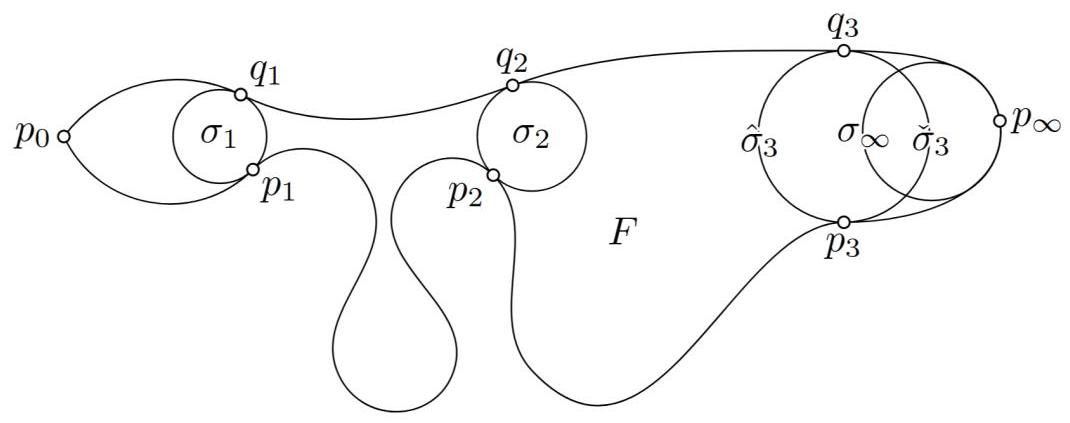
\includegraphics[width=0.8\textwidth]{fig/bo_d3cgcuc601uc738c0ulg_3_224_1244_1070_423_0.jpg}
\end{center}
\hspace*{3em} 

Figure 2. Note that maximal circle \({C}_{p}\) at \(p\) has to touch loop \(c\) at another point \(q\) , but for \({C}_{{p}_{\infty }},{q}_{\infty } = {p}_{\infty } -\) a contradiction.

\begin{tcolorbox}
图2。注意，在点 \(p\) 处的最大圆 \({C}_{p}\) 必须与曲线 \(c\) 在另一点 \(q\) 相切，但对于 \({C}_{{p}_{\infty }},{q}_{\infty } = {p}_{\infty } -\) 来说，这是一个矛盾。
\end{tcolorbox}

\HRule

Theorem 4 ("Moon in the puddle")

\begin{tcolorbox}
定理4(“水坑中的月亮”)
\end{tcolorbox}

\HRule

Let \(c : I \rightarrow  {\mathbb{R}}^{2}\) be a simple, regular loop. If \(\kappa \left( t\right)  \leq  1\) for all \(t \in  I\) , then the region surrounded by \(c\) contains a unit disc.

\begin{tcolorbox}
设 \(c : I \rightarrow  {\mathbb{R}}^{2}\) 为一个简单、规则的闭合曲线。如果对于所有 \(t \in  I\) ，都满足 \(\kappa \left( t\right)  \leq  1\) ，那么由 \(c\) 包围的区域包含一个单位圆盘。
\end{tcolorbox}

Proof | By the lemma, there exists a point \(p = c\left( {t}_{0}\right)\) on the curve such that the osculating circle \(\sigma\) at \(p\) lies inside of \(c\) . But \(\sigma\) has radius \(r = 1/\kappa \left( {t}_{0}\right)  \geq  1\) , so it contains a unit disc.

\begin{tcolorbox}
证明| 根据引理，存在曲线上的一点 \(p = c\left( {t}_{0}\right)\) ，在该点的切线圆 \(\sigma\) 位于 \(c\) 内部。但 \(\sigma\) 的半径为 \(r = 1/\kappa \left( {t}_{0}\right)  \geq  1\) ，因此它包含一个单位圆盘。
\end{tcolorbox}

\section*{Winding number}

\begin{tcolorbox}
\section*{绕数}
\end{tcolorbox}

Another common theme in differential geometry is that the integral of a local quantity over a closed curve or surface often yields a discrete global invariant of the object.

\begin{tcolorbox}
微分几何中的另一个常见主题是，局部量在闭合曲线或曲面上的积分常常产生对象的离散全局不变量。
\end{tcolorbox}

For example, consider a simple loop \(c : \left\lbrack  {a,b}\right\rbrack   \rightarrow  {\mathbb{R}}^{2}\) in the plane that does not pass through the origin. Then we can look at the expression

\begin{tcolorbox}
例如，考虑平面中的一个不经过原点的简单闭合曲线 \(c : \left\lbrack  {a,b}\right\rbrack   \rightarrow  {\mathbb{R}}^{2}\) 。然后我们可以观察表达式
\end{tcolorbox}

\[
\frac{1}{2\pi }{\int }_{a}^{b}\frac{x\left( t\right) \dot{y}\left( t\right)  - y\left( t\right) \dot{x}\left( t\right) }{x{\left( t\right) }^{2} + y{\left( t\right) }^{2}}\mathrm{\;d}t. \tag{3.1}
\]

A priori, this integral could take any real value. And you might expect that if you deform the curve slightly, the integrand would change continuously, and thus the value of the integral would also change continuously. However, this is not the case. The integral actually takes on only integer values and remains invariant under continuous deformations of the curve that do not pass through the origin.

\begin{tcolorbox}
先验上，这个积分可以取任何实数值。你可能会预期，如果你稍微变形曲线，被积函数会连续变化，因此积分的值也会连续变化。然而，事实并非如此。这个积分实际上只取整数值，并且在不经过原点的连续变形下保持不变。
\end{tcolorbox}

To understand why this is true, it is helpful to start from the following geometric notion.

\begin{tcolorbox}
为了理解为什么会这样，有助于从以下几何概念入手。
\end{tcolorbox}

\HRule

Definition 8 (Winding number)

\begin{tcolorbox}
定义8(绕数)
\end{tcolorbox}

\HRule

Let \(c : \left\lbrack  {a,b}\right\rbrack   \rightarrow  {\mathbb{R}}^{2}\) be a loop and \({P}_{0}\) be a point that does not lie on the curve. The winding number \(W\left( {c,{P}_{0}}\right)\) is the number of times the curve goes counter-clockwise around \({P}_{0}\) .

\begin{tcolorbox}
设 \(c : \left\lbrack  {a,b}\right\rbrack   \rightarrow  {\mathbb{R}}^{2}\) 为一条闭合曲线， \({P}_{0}\) 为不在曲线上的一点。绕数 \(W\left( {c,{P}_{0}}\right)\) 是曲线逆时针绕 \({P}_{0}\) 的次数。
\end{tcolorbox}

From geometric considerations, it is clear that the winding number is an integer that satisfies the following properties:

\begin{tcolorbox}
从几何角度来看，很明显绕数是一个满足以下性质的整数:
\end{tcolorbox}

\HRule

Proposition 2

\begin{tcolorbox}
命题2
\end{tcolorbox}

\HRule

\begin{itemize}
\item \(W\left( {c,{P}_{0}}\right)\) depends on \({P}_{0}\) ;
\end{itemize}

\begin{tcolorbox}
\begin{itemize}
\item \(W\left( {c,{P}_{0}}\right)\) 依赖于 \({P}_{0}\) ；
\end{itemize}
\end{tcolorbox}

\begin{itemize}
\item \(W\left( {c,{P}_{1}}\right)  = W\left( {c,{P}_{2}}\right)\) if \({P}_{1}\) and \({P}_{2}\) can be connected by a curve not intersecting \(C\) .
\end{itemize}

\begin{tcolorbox}
\begin{itemize}
\item 如果 \({P}_{1}\) 和 \({P}_{2}\) 可以通过一条不与 \(C\) 相交的曲线相连，则 \(W\left( {c,{P}_{1}}\right)  = W\left( {c,{P}_{2}}\right)\) 相同。
\end{itemize}
\end{tcolorbox}

\begin{itemize}
\item \(W\left( {c,{P}_{0}}\right)\) is invariant under continuous deformations of \(c\) that do not pass through \({P}_{0}\) , i.e., if \({c}_{\delta }\) is a family of loops with \({c}_{\delta }\left( t\right)  \neq  {P}_{0}\) for all \(\delta ,t\) , then \(W\left( {{c}_{\delta },{P}_{0}}\right)\) is independent of \(\delta\) .
\end{itemize}

\begin{tcolorbox}
\begin{itemize}
\item 在不经过 \({P}_{0}\) 的连续变形下， \(W\left( {c,{P}_{0}}\right)\) 保持不变，即如果 \({c}_{\delta }\) 是一族满足 \({c}_{\delta }\left( t\right)  \neq  {P}_{0}\) 的闭合曲线，则 \(W\left( {{c}_{\delta },{P}_{0}}\right)\) 与 \(\delta\) 无关。
\end{itemize}
\end{tcolorbox}

To get a formula for the winding number, we first shift the curve so that \({P}_{0}\) is at the origin. Then we can express the curve in polar coordinates \({}^{1}c\left( t\right)  = r\left( t\right) \left( {\cos \theta \left( t\right) ,\sin \theta \left( t\right) }\right)\) with \(r\left( t\right)  > 0\) for all \(t\) . Since the curve is a loop, we have \(r\left( a\right)  = r\left( b\right)\) and \(\theta \left( b\right)  = \theta \left( a\right)  + {2k\pi }\) for some integer \(k\) . Clearly \(k\) is the winding number of \(c\) around the origin. To find a formula for \(k = \frac{\theta \left( b\right)  - \theta \left( a\right) }{2\pi }\) , we will find an expression for \(\dot{\theta }\left( t\right)\) and then integrate it over \(\left\lbrack  {a,b}\right\rbrack\) . Denoting the components of \(c\left( t\right)\) by \(x\left( t\right)\) and \(y\left( t\right)\) , we have

\begin{tcolorbox}
为了得到绕数的公式，首先将曲线平移，使得 \({P}_{0}\) 位于原点。然后可以用极坐标 \({}^{1}c\left( t\right)  = r\left( t\right) \left( {\cos \theta \left( t\right) ,\sin \theta \left( t\right) }\right)\) 表示曲线，其中 \(r\left( t\right)  > 0\) 对所有 \(t\) 成立。由于曲线是闭合的，我们有 \(r\left( a\right)  = r\left( b\right)\) 和 \(\theta \left( b\right)  = \theta \left( a\right)  + {2k\pi }\) ，其中 \(k\) 是某个整数。显然， \(k\) 是 \(c\) 绕原点的绕数。为了找到 \(k = \frac{\theta \left( b\right)  - \theta \left( a\right) }{2\pi }\) 的公式，我们将找到 \(\dot{\theta }\left( t\right)\) 的表达式，然后在 \(\left\lbrack  {a,b}\right\rbrack\) 上对其积分。用 \(c\left( t\right)\) 的分量用 \(x\left( t\right)\) 和 \(y\left( t\right)\) 表示，我们有
\end{tcolorbox}

\[
\left( \begin{array}{l} \dot{x} \\  \dot{y} \end{array}\right)  = \dot{c} = \dot{r}\left( \begin{matrix} \cos \theta \\  \sin \theta  \end{matrix}\right)  + r\dot{\theta }\left( \begin{matrix}  - \sin \theta \\  \cos \theta  \end{matrix}\right)  \tag{3.2}
\]

\[
= \frac{\dot{r}}{r}\left( \begin{array}{l} x \\  y \end{array}\right)  + \dot{\theta }\left( \begin{matrix}  - y \\  x \end{matrix}\right) .
\]

\customfootnote{

\({}^{1}\) Strictly speaking, we view \(\theta\) here as a smooth real-valued function of \(t\) (and not modulo \({2\pi }\) ). This is possible because the polar coordinates furnish a covering map \(\left( {r,\theta }\right)  \mapsto  r\left( {\cos \theta ,\sin \theta }\right)\) from \(\left( {0,\infty }\right)  \times  \mathbb{R}\) to \({\mathbb{R}}^{2} \smallsetminus  \{ 0\}\) . Then, using the lifting property of covering spaces, we can lift the curve \(c\) in \({\mathbb{R}}^{2} \smallsetminus  \{ 0\}\) to a curve in \(\left( {0,\infty }\right)  \times  \mathbb{R}\) , whose coordinates are exactly the functions \(r\left( t\right)\) and \(\theta \left( t\right)\) .

\begin{tcolorbox}
\({}^{1}\) 严格来说，我们将 \(\theta\) 视为关于 \(t\) 的光滑实值函数(而非模 \({2\pi }\) 的函数)。这是可能的，因为极坐标提供了从 \(\left( {0,\infty }\right)  \times  \mathbb{R}\) 到 \({\mathbb{R}}^{2} \smallsetminus  \{ 0\}\) 的覆盖映射 \(\left( {r,\theta }\right)  \mapsto  r\left( {\cos \theta ,\sin \theta }\right)\) 。然后，利用覆盖空间的提升性质，我们可以将 \({\mathbb{R}}^{2} \smallsetminus  \{ 0\}\) 中的曲线 \(c\) 提升到 \(\left( {0,\infty }\right)  \times  \mathbb{R}\) 中的一条曲线，其坐标正是函数 \(r\left( t\right)\) 和 \(\theta \left( t\right)\) 。
\end{tcolorbox}

}

Taking the dot product of both sides with(-y, x), we conclude that

\begin{tcolorbox}
两边取点积与(-y, x)，我们得出结论
\end{tcolorbox}

\[
\dot{\theta } = \frac{x\dot{y} - y\dot{x}}{{x}^{2} + {y}^{2}}. \tag{3.3}
\]

To find the winding number, we can integrate \(\dot{\theta }\) :

\begin{tcolorbox}
为了求绕数(winding number)，我们可以对 \(\dot{\theta }\) 进行积分:
\end{tcolorbox}

\[
W\left( {c,0}\right)  = \frac{\theta \left( b\right)  - \theta \left( a\right) }{2\pi } = \frac{1}{2\pi }{\int }_{a}^{b}\frac{x\dot{y} - y\dot{x}}{{x}^{2} + {y}^{2}}\mathrm{\;d}t. \tag{3.4}
\]

This is exactly the integral we started with!

\begin{tcolorbox}
这正是我们一开始所用的积分！
\end{tcolorbox}

Section 4

\begin{tcolorbox}
第4节
\end{tcolorbox}

Frenet-Serret frames for curves in \({\mathbb{R}}^{3}\)

\begin{tcolorbox}
曲线在 \({\mathbb{R}}^{3}\) 中的弗雷内-塞雷(Frenet-Serret)框架
\end{tcolorbox}

Curves in \({\mathbb{R}}^{3}\) can

\begin{tcolorbox}
在 \({\mathbb{R}}^{3}\) 中的曲线可以
\end{tcolorbox}

\begin{itemize}
\item bend: measured by curvature (how much the curve deviates from being a straight line in a plane)
\end{itemize}

\begin{tcolorbox}
\begin{itemize}
\item 弯曲:由曲率(衡量曲线偏离直线的程度)来测量
\end{itemize}
\end{tcolorbox}

\begin{itemize}
\item twist: measured by torsion (how much this plane rotates along the curve)
\end{itemize}

\begin{tcolorbox}
\begin{itemize}
\item 扭转:由挠率(衡量沿曲线旋转的平面程度)来测量
\end{itemize}
\end{tcolorbox}

\HRule

Definition 9 (Frenet-Serret frame)

\begin{tcolorbox}
定义9(弗雷内-塞雷框架)
\end{tcolorbox}

\HRule

Let \(c\) be a unit-speed curve in \({\mathbb{R}}^{3},T\left( t\right)  = \dot{c}\left( t\right)\) be the tangent field, curvature \(\kappa \left( t\right)  =\)  \(\left| {\ddot{c}\left( t\right) }\right|\) . Assume \(\kappa \left( t\right)  > 0\) , then \(N\left( t\right)  = \frac{\ddot{c}\left( t\right) }{\left| \ddot{c}\left( t\right) \right| }\) , and \(B\left( t\right)  = T\left( t\right)  \times  N\left( t\right)\) is the binormal field. Here \(\{ T,N,B\}\) is called the Frenet-Serret frame.

\begin{tcolorbox}
设 \(c\) 为一条单位速度的曲线， \({\mathbb{R}}^{3},T\left( t\right)  = \dot{c}\left( t\right)\) 为切向场，曲率为 \(\kappa \left( t\right)  =\)  \(\left| {\ddot{c}\left( t\right) }\right|\) 。假设 \(\kappa \left( t\right)  > 0\) ，则 \(N\left( t\right)  = \frac{\ddot{c}\left( t\right) }{\left| \ddot{c}\left( t\right) \right| }\) ，而 \(B\left( t\right)  = T\left( t\right)  \times  N\left( t\right)\) 为二法向场。这里 \(\{ T,N,B\}\) 称为弗雷内-塞雷(Frenet-Serret)框架。
\end{tcolorbox}

\(T\left( t\right) ,N\left( t\right) ,B\left( t\right)\) are orthogonal to each other and have unit length; notice that \(\left| {v \times  w}\right|  =\)  \(\left( {v,v}\right) \left( {w,w}\right)  - {\left( v,w\right) }^{2}\) .

\begin{tcolorbox}
\(T\left( t\right) ,N\left( t\right) ,B\left( t\right)\) 彼此正交且长度为单位；注意 \(\left| {v \times  w}\right|  =\)  \(\left( {v,v}\right) \left( {w,w}\right)  - {\left( v,w\right) }^{2}\) 。
\end{tcolorbox}

\HRule

Theorem 5 (Frenet-Serret equations)

\begin{tcolorbox}
定理5(弗雷内-塞雷方程)
\end{tcolorbox}

\HRule

If \(c : I \rightarrow  {\mathbb{R}}^{3}\) is a unit-speed curve with \(\mathrm{F} - \mathrm{N}\) frame \(T,N,B\) , then

\begin{tcolorbox}
如果 \(c : I \rightarrow  {\mathbb{R}}^{3}\) 是一条单位速度的曲线，且具有 \(\mathrm{F} - \mathrm{N}\) 框架 \(T,N,B\) ，那么
\end{tcolorbox}

\[
\frac{\mathrm{d}}{\mathrm{d}t}\left( \begin{array}{l} T \\  N \\  B \end{array}\right)  = \left( \begin{matrix} 0 & \kappa & 0 \\   - \kappa & 0 & \tau \\  0 &  - \tau & 0 \end{matrix}\right) \left( \begin{array}{l} T \\  N \\  B \end{array}\right)  \tag{4.1}
\]

where \(\tau \left( t\right)  =  - \dot{B}\left( t\right)  \cdot  N\left( t\right)  = \dot{N}\left( t\right)  \cdot  B\left( t\right)\) is called the torsion of \(c\) at \(t\) .

\begin{tcolorbox}
其中 \(\tau \left( t\right)  =  - \dot{B}\left( t\right)  \cdot  N\left( t\right)  = \dot{N}\left( t\right)  \cdot  B\left( t\right)\) 被称为 \(c\) 在 \(t\) 处的挠率(torsion)。
\end{tcolorbox}

Remark The matrix

\begin{tcolorbox}
备注:该矩阵
\end{tcolorbox}

\[
\Omega  = \left( \begin{matrix} 0 & \kappa & 0 \\   - \kappa & 0 & \tau \\  0 &  - \tau & 0 \end{matrix}\right)  \tag{4.2}
\]

tells us how the Frenet-Serret frame changes along the curve. So if \(T,N,B\) are the frame vectors at time \(t\) , then at time \(t + {\Delta t}\) , the frame vectors are approximately

\begin{tcolorbox}
告诉我们弗雷内-塞雷(Frenet-Serret)框架沿曲线的变化情况。因此，如果 \(T,N,B\) 是时间 \(t\) 时的框架向量，那么在时间 \(t + {\Delta t}\) 时，框架向量大致为
\end{tcolorbox}

\[
\left( {1 + {\Delta t\Omega }}\right) \left( \begin{array}{l} T \\  N \\  B \end{array}\right) . \tag{4.3}
\]

The fact that \(\Omega\) is skew-symmetric (i.e., \({\Omega }^{T} =  - \Omega\) ) means that the transformation \(1 + {\Delta t\Omega }\) is an infinitesimal rotation. Geometrically, this means that as we move along the curve, the Frenet-Serret frame rotates in a way that is determined by the curvature and torsion of the curve.

\begin{tcolorbox}
\(\Omega\) 是反对称的(即， \({\Omega }^{T} =  - \Omega\) )，意味着变换 \(1 + {\Delta t\Omega }\) 是一个无穷小旋转。从几何角度来看，这意味着沿着曲线移动时，弗雷内-塞雷(Frenet-Serret)框架会以由曲线的曲率和挠率决定的方式旋转。
\end{tcolorbox}

Section 7

Exterior differential and Integration of 2-forms

\HRule

Definition 20 (Exterior differential)

\HRule

If \(\alpha\) is a 1-form on \(S\) , then the exterior differential in the \(S\) is defined as

\[
{\left( d\alpha \right) }_{p}\left( {\partial x,\partial y}\right)  = {\mathrm{T}}_{p}\left( {\alpha \left( {\partial y}\right) }\right) \left( {\partial x}\right)  - {\mathrm{T}}_{p}\left( {\alpha \left( {\partial x}\right) }\right) \left( {\partial y}\right)
\]

\[
= {\nabla }_{\partial x}\alpha \left( {\partial y}\right)  - {\nabla }_{\partial y}\alpha \left( {\partial x}\right)
\]

for every chart \(\phi  : D \rightarrow  S\) around \(p\) .

Remark

\[
d\left( {f\alpha }\right)  = {df} \land  \alpha  + {fd\alpha }
\]

\[
d\left( {df}\right)  = 0
\]

1-form is called closed if \({d\alpha } = 0\) , and is called exact if there exists \(f : S \rightarrow  \mathbb{R}\) such that \({df} = \alpha\) . Actually, every exact form is also closed, but not every closed form is exact.

\HRule

Definition 21 (Integration of 2-forms)

\HRule

The integral of the 2-form \(\beta\) over the rectangle \(R\) is

\[
{\int }_{R}\beta  = {\int }_{a}^{b}{\int }_{c}^{d}{\beta }_{R\left( {x,y}\right) }\left( {\frac{\partial R\left( {x,y}\right) }{\partial x},\frac{\partial R\left( {x,y}\right) }{\partial y}}\right) {dydx}
\]

where \(\frac{\partial R\left( {x,y}\right) }{\partial x}\) is the tangent vector at \(R\left( {x,y}\right)  \in  S\) given by the curve \(t \rightarrow  R\left( {t + x,y}\right)\) , and similar definition for \(\frac{\partial R\left( {x,y}\right) }{\partial y}\) .

We shall ask: "what does \({\int }_{R}\beta\) computes?" Let

\[
\beta  = {F}_{1}{dy} \land  {dz} + {F}_{2}{dz} \land  {dx} + {F}_{3}{dx} \land  {dy}
\]

be a 2-form on \(U \subseteq  {\mathbb{R}}^{3}\) with smooth function \({F}_{i} : U \rightarrow  \mathbb{R}\) . We may think of \(F = \; \left( {{F}_{1},{F}_{2},{F}_{3}}\right)  : U \rightarrow  {\mathbb{R}}^{3}\) as a vector field on \(U \subseteq  {\mathbb{R}}^{3}\) . Let \(R : \left\lbrack  {a,b}\right\rbrack   \times  \left\lbrack  {c,d}\right\rbrack   \rightarrow  U\) be a rectangular region, denote

\[
{T}_{x}\left( {x,y}\right)  = \frac{\partial R\left( {x,y}\right) }{\partial x},\;{T}_{y}\left( {x,y}\right)  = \frac{\partial R\left( {x,y}\right) }{\partial y}
\]

Write \({T}_{x} = \left( {{T}_{x}^{1},{T}_{x}^{2},{T}_{x}^{3}}\right)\) , then \({dx}\left( {T}_{x}\right)  = {T}_{x}^{1},{dy}\left( {T}_{x}\right)  = {T}_{x}^{2},{dz}\left( {T}_{x}\right)  = {T}_{x}^{3}\) , therefore

\[
{\int }_{R}\beta  = {\int }_{a}^{b}{\int }_{c}^{d}{\beta }_{R\left( {x,y}\right) }\left( {{T}_{x}\left( {x,y}\right) ,{T}_{y}\left( {x,y}\right) }\right) {dydx}
\]

\[
= {\int }_{a}^{b}{\int }_{c}^{d}{F}_{1}{dy} \land  {dz}\left( {\frac{\partial R\left( {x,y}\right) }{\partial x},\frac{\partial R\left( {x,y}\right) }{\partial y}}\right) {dydx} + {F}_{2}{dz} \land  {dx}\left( {\frac{\partial R\left( {x,y}\right) }{\partial x},\frac{\partial R\left( {x,y}\right) }{\partial y}}\right) {dydx}
\]

\[
+ {F}_{3}{dx} \land  {dy}\left( {\frac{\partial R\left( {x,y}\right) }{\partial x},\frac{\partial R\left( {x,y}\right) }{\partial y}}\right) {dydx}
\]

\[
= {\int }_{a}^{b}{\int }_{c}^{d}{F}_{1}\left( {{T}_{x}^{2}{T}_{y}^{3} - {T}_{x}^{3}{T}_{y}^{2}}\right) {dydx} + {F}_{2}\left( {{T}_{x}^{3}{T}_{y}^{1} - {T}_{x}^{1}{T}_{y}^{3}}\right) {dydx} + {F}_{3}\left( {{T}_{x}^{1}{T}_{y}^{2} - {T}_{x}^{2}{T}_{y}^{1}}\right) {dydx}
\]

\[
= {\int }_{a}^{b}{\int }_{c}^{d}F\left( {R\left( {x,y}\right) }\right)  \cdot  n\left( {x,y}\right) {dydx}
\]

which is the classical surface integral over the vector field \(F =\) flux of \(F\) through the rectangle \(R\) .

Suppose \(U \subseteq  {\mathbb{R}}^{2}\) open, \(\alpha\) a 2-form on \(U\) . Let \(R : \left\lbrack  {a,b}\right\rbrack   \times  \left\lbrack  {c,d}\right\rbrack\) injective and s.t. the det of jacobian is positive. Let \(\partial R\) be the boundary curve of \(R\) , then

\[
{\int }_{R}{d\alpha } = {\int }_{\partial R}\alpha
\]

\HRule

Theorem 7

(Green's thm)

\HRule

which corresponds to the stokes formula

\[
{\int }_{R}\operatorname{curl}V \cdot  {ndA} = {\int }_{\partial R}{Vdl}
\]

roof Let \(\alpha  = {\alpha }_{1}{dx} + {\alpha }_{2}{dy}\) , then

\[
{d\alpha } = d{\alpha }_{1} \land  {dx} + d{\alpha }_{2} \land  {dy} = \frac{\partial {\alpha }_{1}}{\partial y}{dy} \land  {dx} + \frac{\partial {\alpha }_{2}}{\partial x}{dx} \land  {dy} = \left( {\frac{\partial {\alpha }_{2}}{\partial x} - \frac{\partial {\alpha }_{1}}{\partial y}}\right) {dx} \land  {dy}
\]

therefore

\[
{\int }_{R}{d\alpha } = {\int }_{a}^{b}{\int }_{c}^{d}{\left( d\alpha \right) }_{R\left( {x,y}\right) }\left( {\frac{\partial R\left( {x,y}\right) }{\partial x},\frac{\partial R\left( {x,y}\right) }{\partial y}}\right) {dydx}
\]

\[
= {\int }_{a}^{b}{\int }_{c}^{d}\left( {\frac{\partial {\alpha }_{2}}{\partial x}\left( {R\left( {x,y}\right) }\right)  - \frac{\partial {\alpha }_{1}}{\partial y}\left( {R\left( {x,y}\right) }\right) }\right) \left( {\frac{\partial {R}_{1}}{\partial x}\frac{\partial {R}_{2}}{\partial y} - \frac{\partial {R}_{2}}{\partial x}\frac{\partial {R}_{1}}{\partial y}}\right) {dydx}
\]

\[
= {\int }_{a}^{b}{\int }_{c}^{d}\left( {\frac{\partial {\alpha }_{2}}{\partial x}\left( {R\left( {x,y}\right) }\right)  - \frac{\partial {\alpha }_{1}}{\partial y}\left( {R\left( {x,y}\right) }\right) }\right) \det \left( {\frac{\partial R}{\partial x},\frac{\partial R}{\partial y}}\right) {dydx}
\]

\[
= {\iint }_{R\left( {\left\lbrack  {a,b}\right\rbrack   \times  \left\lbrack  {c,d}\right\rbrack  }\right) }\left( {\frac{\partial {\alpha }_{2}}{\partial x} - \frac{\partial {\alpha }_{1}}{\partial y}}\right) {dydx}
\]

\[
= {\int }_{\partial R}{\alpha }_{1}{dx} + {\alpha }_{2}{dy}
\]

\[
= {\int }_{\partial R}\alpha
\]

Cartan's moving frames

Recall for curves, we had a moving frame (Cartan) at every point of curve (T, N, B), which was adapted the curve \(\left( {\mathrm{T} = \dot{c}}\right)\) . The change of this frame, expanded in terms of the frame, told us the curvature and the torsion of the curve. For the surface, the idea is to do something similar to get the curvature of a surface.

Definition 22 (Moving frame)

A moving frame on an open subset \(U \subseteq  {\mathbb{R}}^{3}\) consists of vector fields \({e}_{1},{e}_{2},{e}_{3} : U \rightarrow  {\mathbb{R}}^{3}\) such that for each point \(x \in  U\) , the values \({e}_{1}\left( x\right) ,{e}_{2}\left( x\right) ,{e}_{3}\left( x\right)\) are an orthonormal basis of \({\mathbb{R}}^{3}\) .

Definition 23 (Change of frame) Suppose \({e}_{1} : U \rightarrow  {\mathbb{R}}^{3},{e}_{1} = \left( {{f}_{1},{f}_{2},{f}_{3}}\right)\) where \(f : U \rightarrow  \mathbb{R}\) , then

\[
d{e}_{1} = \left( {d{f}_{1},d{f}_{2},d{f}_{3}}\right)
\]

Since \({\left( d{f}_{i}\right) }_{x} : {\mathbb{R}}^{3} \rightarrow  \mathbb{R}\) is linear, hence also \({\left( d{e}_{1}\right) }_{x} = \left( {{\left( d{f}_{1}\right) }_{x},{\left( d{f}_{2}\right) }_{x},{\left( d{f}_{3}\right) }_{x}}\right)  : {\mathbb{R}}^{3} \rightarrow  {\mathbb{R}}^{3}\) is a linear map, and \({\left( d{e}_{1}\right) }_{x}\left( v\right)  = \left( {{\left( d{f}_{1}\right) }_{x}\left( v\right) ,{\left( d{f}_{2}\right) }_{x}\left( v\right) ,{\left( d{f}_{3}\right) }_{x}\left( v\right) }\right)\) shows how the \({e}_{i}\) changes in \(v\) direction.

Definition 24 (Expand change to the frame itself)

Since \({\left( d{e}_{i}\right) }_{x}\left( v\right)  \in  {\mathbb{R}}^{3}\) , and \({e}_{1}\left( x\right) ,{e}_{2}\left( x\right) ,{e}_{3}\left( x\right)\) is a basis of \({\mathbb{R}}^{3}\) , we can expand \({\left( d{e}_{i}\right) }_{x}\left( v\right)\) in terms of \({e}_{j}\left( x\right)\) :

\[
{\left( d{e}_{i}\right) }_{x}\left( v\right)  = \mathop{\sum }\limits_{{j = 1}}^{3}{\left( {\omega }_{i}^{j}\right) }_{x}\left( v\right) {e}_{j}\left( x\right)
\]

as \({e}_{1},{e}_{2},{e}_{3}\) are ONB, we have connection forms:

\[
{\left( {\omega }_{i}^{j}\right) }_{x}\left( v\right)  = {\left( d{e}_{i}\right) }_{x}\left( v\right) {e}_{j}\left( x\right)
\]

hence, \({\left( {\omega }_{i}^{j}\right) }_{x}\left( v\right)\) measures how much the vector \({e}_{i}\left( x\right)\) rotates towards \({e}_{j}\left( x\right)\) direction, and \({\left( {\omega }_{i}^{j}\right) }_{x}\left( v\right)\) is a 1-form for every \(i\) and \(j\) .

It’s easy to say that \({\left( {\omega }_{i}^{j}\right) }_{x}\left( v\right)\) is skew-symmetric:

\[
0 = d{\left( {e}_{i} \cdot  {e}_{j}\right) }_{x}\left( v\right)  = {\left( d{e}_{i}\right) }_{x}\left( v\right)  \cdot  {e}_{j}\left( x\right)  + {e}_{i}\left( x\right)  \cdot  {\left( d{e}_{j}\right) }_{x}\left( v\right)  = {\left( {\omega }_{i}^{j}\right) }_{x}\left( v\right)  + {\left( {\omega }_{j}^{i}\right) }_{x}\left( v\right)
\]

therefore

\[
\left( {\omega }_{i}^{j}\right)  = \left( \begin{matrix} 0 & {\omega }_{1}^{2} & {\omega }_{1}^{3} \\   - {\omega }_{1}^{2} & 0 & {\omega }_{2}^{3} \\   - {\omega }_{1}^{3} &  - {\omega }_{2}^{3} & 0 \end{matrix}\right)
\]

Let \(c\) be a unit-speed curve with \(\kappa  > 0\) . Suppose that \({e}_{1},{e}_{2},{e}_{3}\) is a moving frame on \({\mathbb{R}}^{3}\) such that the restriction to \(c\) gives the Frenet-Serret frame, then

\[
{\left( {w}_{1}^{2}\right) }_{c\left( t\right) }\left( T\right)  = \kappa \left( t\right)
\]

\[
{\left( {w}_{1}^{3}\right) }_{c\left( t\right) }\left( T\right)  = 0
\]

\[
{\left( {w}_{2}^{3}\right) }_{c\left( t\right) }\left( T\right)  = \tau \left( t\right)
\]

which says that \({e}_{1}\left( { = T}\right)\) doesn’t tip in \({e}_{3}\left( { = B}\right)\) direction.

Let \(f = \left\lbrack  {{f}_{1},{f}_{2},{f}_{3}}\right\rbrack\) be the standard basis of \({\mathbb{R}}^{3}\) , and suppose the rotation is described by the attitude matrix \(\left\lbrack  A\right\rbrack   = \left\lbrack  {a}_{ij}\right\rbrack\) , which satisfies \({\left\lbrack  A\right\rbrack  }^{T} = {\left\lbrack  A\right\rbrack  }^{-1}\) , then

\[
\left\lbrack  e\right\rbrack   = \left\lbrack  A\right\rbrack  \left\lbrack  f\right\rbrack
\]

therefore

\[
{\omega }_{i}^{j}\left( v\right)  = \left( {{\nabla }_{v}{e}_{i}}\right)  \cdot  {e}_{j} = \mathop{\sum }\limits_{k}\left( {d{a}_{ik}}\right) \left( v\right) {f}_{k} \cdot  {e}_{j} = \mathop{\sum }\limits_{k}\left( {\left( {d{a}_{ik}}\right) \left( v\right) }\right)  \cdot  {a}_{jk}
\]

i.e.

\[
\left\lbrack  \omega \right\rbrack   = d\left\lbrack  A\right\rbrack   \cdot  {\left\lbrack  A\right\rbrack  }^{T}
\]

The frame \({e}_{1},{e}_{2},{e}_{3}\) is not the most basic object, we want to replace the moving frame field \({e}_{i}\) with its dual 1-form \({\theta }_{i}\) .

Definition 25 (Dual frame) The dual frame are 1-forms \({\theta }_{1},{\theta }_{2},{\theta }_{3}\) on \({\mathbb{R}}^{3}\) such that \({\left( {\theta }_{i}\right) }_{x}\left( {{e}_{j}\left( x\right) }\right)  = {\delta }_{ij}\) .

We know that the attitude matrix \(\left\lbrack  {a}_{ij}\right\rbrack\) transforms the fixed Euclidean basis \(\left\{  {f}_{j}\right\}\) into Cartan’s frame field \(\left\{  {e}_{i}\right\}\) , we now show that the same rotation matrix transforms the 1-form basis \(\left\{  {d{x}_{j}}\right\}\) dual to \(\left\{  {f}_{j}\right\}\) into the 1-form basis \(\left\{  {\theta }_{i}\right\}\) dual to \(\left\{  {e}_{i}\right\}\) :

\[
\left\lbrack  \theta \right\rbrack   = \left\lbrack  A\right\rbrack  \left\lbrack  {dx}\right\rbrack
\]

where

\[
{\theta }_{i} = \mathop{\sum }\limits_{j}{\theta }_{i}\left( {f}_{j}\right) d{x}_{j}
\]

\(\mathop{\sum }\limits_{k}{\omega }_{k}^{i} \land  {\theta }_{k} + d{\theta }_{i} = 0.\)

\[
0 = d\left( {\mathop{\sum }\limits_{{k = 1}}^{3}{\theta }_{k} \cdot  {e}_{k}}\right)
\]

\[
= \mathop{\sum }\limits_{k}\left( {\left( {d{e}_{k}}\right)  \land  {\theta }_{k} + \left( {d{\theta }_{k}}\right) {e}_{k}}\right)
\]

\[
= \mathop{\sum }\limits_{k}\left( {\mathop{\sum }\limits_{i}\left( {{\omega }_{k}^{i}{e}_{i}}\right)  \land  {\theta }_{k} + \left( {d{\theta }_{k}}\right) {e}_{k}}\right)
\]

\[
= \mathop{\sum }\limits_{i}{e}_{i}\left( {\mathop{\sum }\limits_{i}{\omega }_{k}^{i} \land  {\theta }_{k} + d{\theta }_{i}}\right)
\]

\[
d\left\lbrack  \theta \right\rbrack   = \left\lbrack  \omega \right\rbrack   \land  \left\lbrack  \theta \right\rbrack
\]

Differentiating \(\left\lbrack  \theta \right\rbrack   = \left\lbrack  A\right\rbrack  \left\lbrack  {dx}\right\rbrack\) , then

\[
d\left\lbrack  \theta \right\rbrack   = d\left\lbrack  A\right\rbrack   \land  \left\lbrack  {dx}\right\rbrack   = d\left\lbrack  A\right\rbrack  {\left\lbrack  A\right\rbrack  }^{T} \land  \left\lbrack  A\right\rbrack  \left\lbrack  {dx}\right\rbrack   = \left\lbrack  \omega \right\rbrack   \land  \left\lbrack  \theta \right\rbrack
\]

\HRule

Proposition 5 (The connection forms via the attitude matrix)

Definition 26 (The duals \({\theta }_{i}\) of \({e}_{i}\) in terms of the duals \(d{x}_{j}\) of \(\left. {f}_{j}\right)\)

Theorem 8 (Cartan's first structure equations

Proposition 6

(Cartan's first structure equation proved day attitude matrix)

\HRule

Theorem 9 (Second structure equation? \(\mathop{\sum }\limits_{j}{\omega }_{j}^{k} \land  {\omega }_{i}^{j} + d{\omega }_{i}^{k} = 0\)

\[
0 = d\left( {d{e}_{i}}\right)  = d\left( {\mathop{\sum }\limits_{j}{\omega }_{i}^{j} \cdot  {e}_{j}}\right)
\]

\[
= \mathop{\sum }\limits_{j}\left( {d{e}_{j} \land  {\omega }_{i}^{j} + \left( {d{\omega }_{i}^{j}}\right) {e}_{j}}\right)
\]

\[
= \mathop{\sum }\limits_{j}\left( {\mathop{\sum }\limits_{k}\left( {{\omega }_{j}^{k}{e}_{k}}\right)  \land  {\omega }_{i}^{j} + \left( {d{\omega }_{i}^{j}}\right) {e}_{j}}\right)
\]

\[
= \mathop{\sum }\limits_{k}{e}_{k}\left( {\mathop{\sum }\limits_{j}{\omega }_{j}^{k} \land  {\omega }_{i}^{j} + d{\omega }_{i}^{k}}\right)
\]

Proposition 7

(Cartan's second structure equationf proved by attitude matrix)

\[
d\left\lbrack  \omega \right\rbrack   = \left\lbrack  \omega \right\rbrack   \land  \left\lbrack  \omega \right\rbrack
\]

Differentiating \(\left\lbrack  \omega \right\rbrack\) , then

\[
d\left\lbrack  \omega \right\rbrack   = d\left\lbrack  {\left( {d\left\lbrack  A\right\rbrack  }\right) {\left\lbrack  A\right\rbrack  }^{T}}\right\rbrack
\]

\[
=  - \left( {d\left\lbrack  A\right\rbrack  }\right)  \land  d{\left\lbrack  A\right\rbrack  }^{T}
\]

\[
=  - \left( {d\left\lbrack  A\right\rbrack  }\right) {\left\lbrack  A\right\rbrack  }^{T} \land  \left\lbrack  A\right\rbrack  d{\left\lbrack  A\right\rbrack  }^{T}
\]

\[
=  - \left( {d\left\lbrack  A\right\rbrack  }\right) {\left\lbrack  A\right\rbrack  }^{T} \land  {\left\lbrack  \left( d\left\lbrack  A\right\rbrack  \right) {\left\lbrack  A\right\rbrack  }^{T}\right\rbrack  }^{T}
\]

\[
=  - \left\lbrack  \omega \right\rbrack   \land  {\left\lbrack  \omega \right\rbrack  }^{T}
\]

\[
= \left\lbrack  \omega \right\rbrack   \land  \left\lbrack  \omega \right\rbrack
\]

Gauss map and shape operator

Similar to study curves through Frenet-Serret frame, we use the Cartan method to study the surface \(S\) , and the strategy is to put frames on \(S\) (adapted), then study the rate of the frame's change.

Recall that if \(S\) is a surface that is oriented, then there exists a normal field \(n : S \rightarrow \; {\mathbb{R}}^{3}\) , which vanishes nowhere, so we can define a map from \(p \in  S\) to the normal vector \(n\left( p\right)\) at this point, which is called Gauss map.

If \(n\left( p\right)\) has unit norm for \(\forall p \in  S\) , then we call \(n : S \rightarrow  {S}^{2} \subseteq  {\mathbb{R}}^{3}\) the gauss map of \(S\) . Moreover, for the surface \(\phi  : D \rightarrow  S\) , gauss map \(n\) can be written as

\[
n\left( {u,v}\right)  \mathrel{\text{ := }} \frac{\frac{\partial \phi }{\partial u} \times  \frac{\partial \phi }{\partial v}}{\begin{Vmatrix}\frac{\partial \phi }{\partial u} \times  \frac{\partial \phi }{\partial v}\end{Vmatrix}}
\]

\HRule

Definition 27

(Gauss map)

\HRule

Remark

If \(n : S \rightarrow  {S}^{2}\) is the gauss map, and \({e}_{1},{e}_{2},{e}_{3}\) a frame on \({\mathbb{R}}^{3}\) , then this frame is adapted to \(S\) if and only if \(n\left( p\right)  = {e}_{3}\left( p\right)\) .

Example

Consider the cylinder \(S = \left\{  {\left( {x,y,z}\right)  : {x}^{2} + {y}^{2} = {r}^{2}}\right\}\) , and the tangent space \(V \subseteq  {\mathbb{R}}^{3}\) is tangent to \(S\) at \(p = \left( {x,y,z}\right)  \in  S\) iff there is a curve \(c\left( t\right)  \in  S\) satisfying \(c\left( 0\right)  = p,\dot{c}\left( 0\right)  = \; v \in  V\) . If \(c\left( t\right)  = \left( {x\left( t\right) ,y\left( t\right) ,z\left( t\right) }\right)\) , then \(x{\left( t\right) }^{2} + y{\left( t\right) }^{2} = {r}^{2}\) , and take derivative, we get

\[
x \cdot  {v}_{1} + y \cdot  {v}_{2} = 0
\]

hence

\[
{v}_{1} = {ya},\;{v}_{2} =  - {xa},\;{v}_{3}\text{ arbitrary }
\]

for some constant \(a \in  \mathbb{R}\) . Therefore, the tangent space of \(S\) is spanned by

\[
y\partial x - x\partial y,\;\partial z
\]

for \(\left( {x,y,z}\right)  \in  S\) , and the normal field \(n : S \rightarrow  {\mathbb{R}}^{3}\) is \(n = x\partial x + y\partial y\) , thus for example

\[
{e}_{1} = \partial z,\;{e}_{2} = {e}_{1} \times  {e}_{3},\;{e}_{3} = \frac{x\partial x + y\partial y}{\sqrt{{x}^{2} + {y}^{2}}}
\]

is a frame on \({\mathbb{R}}^{3} \smallsetminus  \{ 0\}\) adapted for \(S\) .

\HRule

Lemma 4 (Moving frame and tangent vector field)

\HRule

Let \(S\) be a oriented surface with unit normal \(n\) , then there exists an adapted moving frame on open subset \(\mathcal{O} \subseteq  S\) if and only if there exists a non-vanishing tangent vector field \(v\) on \(\mathcal{O}\left( {{v}_{p} \in  {\mathrm{T}}_{p}S}\right)\) .

Proof \(\Rightarrow\) : If \(\left( {{e}_{1},{e}_{2},{e}_{3}}\right)\) is an adapted moving frame, \({e}_{1}\left( p\right)  \in  {\mathrm{T}}_{p}S\) and never vanishes.

\(\Leftarrow\) : If \(v\) is nowhere vanishing on \(\mathcal{O} \subseteq  S\) , then

\[
{e}_{1} = \frac{v}{\parallel v\parallel },\;{e}_{2} = {e}_{1} \times  n,\;{e}_{3} = n
\]

is an adapted frame on \(\mathcal{O}\) .

\HRule

"As we have seen in Chapter 1, the consideration of the rate of change of the tangent line to a curve \(c\) led us to an important ge-ornetric entity, namely, the curvature of \(c\) . In this chapter we shall extend this idea to regular surfaces; that is, we shall try to measure how rapidly a surface \(S\) pulls away from the tangent plane \({\mathrm{T}}_{p}S\) in a neighborhood of a point \(p \in  S\) . This is equivalent to measuring the rate of change at \(p\) os a unit normal vector field \(N\) on a neighborhood of \(p\) . As we shall see shortly, this rate of change is given by a linear map on \({\mathrm{T}}_{p}S\) which happens to be self-adjoint. A surprisingly large number of local properties of \(S\) at \(p\) can be derived from the study of this linear map."

Selected from do Carmo, Differential Geometry of Curves and Surfaces, page 134

\HRule

If \({e}_{1},{e}_{2},{e}_{3}\) is an adapted frame \(\mathcal{O} \in  {\mathbb{R}}^{3}\) , then

\[
{\left( d{e}_{i}\right) }_{p}\left( v\right)  = \mathop{\sum }\limits_{j}{\left( {\omega }_{i}^{j}\right) }_{p}\left( v\right) {e}_{j}\left( p\right) \;\text{ for }p \in  \mathcal{O} \cap  S,v \in  {\mathrm{T}}_{p}S \subseteq  {\mathbb{R}}^{3}.
\]

For curves, only needed points on the curve and \(v = T\) , the tangent direction to recover the curvature and torsion of the curve, but for the surfaces, we have two tangent directions. Because of the anti-symmetry of \(\left( {\omega }_{i}^{j}\right)\) , the only independent elements are \({\omega }_{1}^{2},{\omega }_{1}^{3},{\omega }_{2}^{3}\) , where \({\omega }_{1}^{2}\) measures how much \({e}_{1}\) changes in \({e}_{2}\) direction, showing the information about \({\mathrm{T}}_{p}S\) , which is "intrinsic"; while \({\omega }_{1}^{3},{\omega }_{2}^{3}\) measures how \({e}_{3}\) changes in \({e}_{1},{e}_{2}\) direction, showing the change of the gauss map/normal vector field, which is "extrinsic".

\HRule

Definition 28 (Shape operator)

\HRule

The shape operator (Weingarten map)

\[
{\mathcal{S}}_{p} =  - {\mathrm{T}}_{p}n =  - \nabla {n}_{p} : {\mathrm{T}}_{p}S \rightarrow  {\mathrm{T}}_{p}S
\]

measures the change of \(n : S \rightarrow  {S}^{2}\) , and

\[
{\mathcal{S}}_{p}\left( v\right)  =  - {\nabla }_{v}{n}_{p} =  - d{n}_{p} \cdot  v =  - {\left. \left( \frac{\partial n}{\partial x},\frac{\partial n}{\partial y},\frac{\partial n}{\partial z}\right) \right| }_{\left( {x,y,z}\right)  = p} \cdot  v
\]

\[
=  - \nabla n\left( {c\left( 0\right) }\right)  \cdot  \dot{c}\left( 0\right)  =  - {\left. \frac{\mathrm{d}}{\mathrm{d}t}\right| }_{t = 0}n\left( {c\left( t\right) }\right)  =  - {\left. \mathop{\sum }\limits_{{i = 1}}^{3}\frac{\mathrm{d}}{\mathrm{d}t}\right| }_{t = 0}{n}^{i}\left( {c\left( t\right) }\right) {e}_{i}
\]

If \(\left( {{e}_{1},{e}_{2},{e}_{3}}\right)\) is an adapted frame, then \({e}_{3} = n\)

\[
{\mathcal{S}}_{p}\left( v\right)  =  - {\left( d{e}_{3}\right) }_{p}\left( v\right)  = {\left( {\omega }_{1}^{3}\right) }_{p}\left( v\right) {e}_{1}\left( p\right)  + {\left( {\omega }_{2}^{3}\right) }_{p}\left( v\right) {e}_{2}\left( p\right)
\]

therefore, the shape operator is the analog of curvature/torsion of a curve: \(\kappa ,\tau\) tell us how \(T\) and \(B\) are changing in \(N\) direction, while \(\mathcal{S}\) tells us how \(n\) is changing in the two tangent directions.

\[
I{I}_{p}\left( {v,w}\right)  = v \cdot  {\mathcal{S}}_{p}\left( w\right)  = {I}_{p}\left( {v,{\mathcal{S}}_{p}\left( w\right) }\right) ,p \in  S,v,w \in  {\mathrm{T}}_{p}S.
\]

\begin{center}
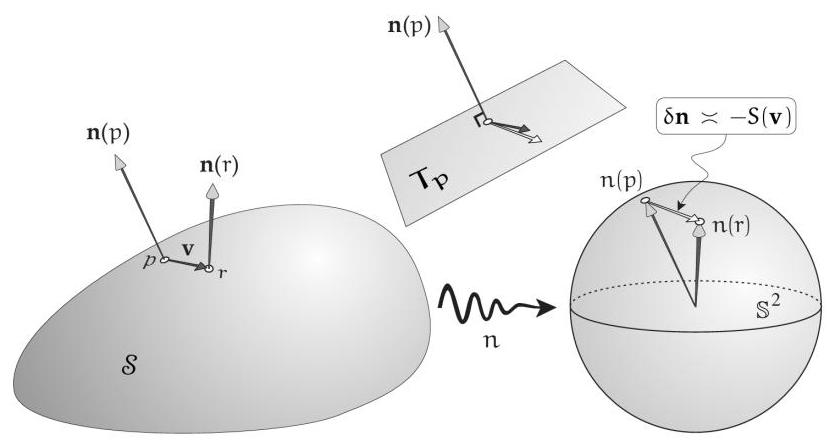
\includegraphics[width=0.6\textwidth]{fig/bo_d4vqblv7aajc73ft760g_6_333_1362_831_440_0.jpg}
\end{center}
\hspace*{3em} 

Figure 5. The Shape Operator applied to a short tangent vector \(v\) emanating from \(p\) in \({\mathrm{T}}_{p}S\) tells us how much the normal changes from the tail to the tip of \(v\) . This change \({\delta n} \approx   - \mathcal{S}\left( v\right)\) ultimately lies in the parallel tangent plane to \({S}^{2}\) at \(n\left( p\right)\) . Superimposing the two tangent planes, \(S\) may be viewed as a linear transformation of \({\mathrm{T}}_{p}S\) to itself, here depicted detached from \(S\) , floating between the two surfaces.

Proposition 8 ( \({\mathcal{S}}_{p}\) is a self-adjoint linear operator) For each point \(p\) of \(S \subseteq  {\mathbb{R}}^{3}\) , the shape operator is a self-adjoint linear operator

\[
{\mathcal{S}}_{p} : {\mathrm{T}}_{p}S \rightarrow  {\mathrm{T}}_{p}S
\]

on the tangent plane of \(S\) at \(p\) .

Proof

As \(n\) is a unit vector field, \({n}_{p} \cdot  {n}_{p} = 1\) for any \(p \in  S\) , thus by a Leibniz property of covariant derivatives

\[
0 = {\nabla }_{v}\left( {{n}_{p} \cdot  {n}_{p}}\right)  = 2\left( {{\nabla }_{v}{n}_{p}}\right)  \cdot  {n}_{p} =  - 2{\mathcal{S}}_{p}\left( v\right)  \cdot  {n}_{p}
\]

where \(v\) is tangent to \(S\) at \(p\) , thus \({\mathcal{S}}_{p}\) is a function from \({\mathrm{T}}_{p}S\) to \({\mathrm{T}}_{p}S\) . The linearity of \({\mathcal{S}}_{p}\) is a consequence of a linearity property of covariant derivatives:

\[
{\mathcal{S}}_{p}\left( {{av} + {bw}}\right)  =  - {\nabla }_{{av} + {bw}}{n}_{p} =  - \left( {a{\nabla }_{v}{n}_{p} + b{\nabla }_{w}{n}_{p}}\right)  = a{\mathcal{S}}_{p}\left( v\right)  + b{\mathcal{S}}_{p}\left( w\right)
\]

Suppose \(\left\{  {{x}_{u},{x}_{v}}\right\}\) are the associated basis of \({\mathrm{T}}_{p}S\) , then \(\left( {n,{x}_{u}}\right)  = 0 = \left( {n,{x}_{v}}\right)\) , take the derivatives of them relative to \(v\) and \(u\) , obtain

\[
\left( {{n}_{v},{x}_{u}}\right)  + \left( {n,{x}_{uv}}\right)  = 0
\]

\[
\left( {{n}_{u},{x}_{v}}\right)  + \left( {n,{x}_{vu}}\right)  = 0
\]

thus

\[
\left( {{n}_{u},{x}_{v}}\right)  =  - \left( {n,{x}_{vu}}\right)  = \left( {{n}_{v},{x}_{u}}\right)
\]

Example

Sphere of radius \(R\) has gauss map \({n}_{p} = \frac{p}{R},{n}_{p} \cdot  {n}_{p} = 1\) , so

\[
{\mathcal{S}}_{p}\left( v\right)  =  - {\mathrm{T}}_{p}n\left( v\right)  =  - {\left. \frac{\mathrm{d}}{\mathrm{d}t}\right| }_{t = 0}n\left( {c\left( t\right) }\right)  =  - {\left. \frac{\mathrm{d}}{\mathrm{d}t}\right| }_{t = 0}\frac{c\left( t\right) }{R} =  - \frac{v}{R}
\]

which doesn’t depend on \(p\) , and gets small if \(R \rightarrow   + \infty\) .

Proposition 9 ("Detection of curvature via acceleration") If \(c : I \rightarrow  S\) is a smooth curve in \(S\) , then

\[
\ddot{c}\left( t\right)  \cdot  n\left( {c\left( t\right) }\right)  = \dot{c}\left( t\right)  \cdot  {\mathcal{S}}_{c\left( t\right) }\left( {\dot{c}\left( t\right) }\right)
\]

Proof if \(c\) in \(S\) , then \(\dot{c}\left( t\right)  \in  {T}_{c\left( t\right) }S\) , thus

\[
\dot{c}\left( t\right)  \cdot  n\left( {c\left( t\right) }\right)  = 0
\]

\({\left. \frac{\mathrm{d}}{\mathrm{d}t}\right| }_{t} :\)

\[
\ddot{c}\left( t\right)  \cdot  n\left( {c\left( t\right) }\right)  + \dot{c}\left( t\right)  \cdot  {T}_{c\left( t\right) }n\left( {\dot{c}\left( t\right) }\right)  = 0
\]

therefore, all curves in \(S\) with a given velocity \(v\) at \(p\) have the same acceleration in the normal direction, namely \(v \cdot  {\mathcal{S}}_{p}\left( v\right)\) . This normal accelaration comes from the fact that the curve has to stay at the surface and is determined by geometry of the surface.

Definition 29 (The first fundamental form)

\[
{I}_{p}\left( {v,w}\right)  = v \cdot  w,p \in  S,v,w \in  {\mathrm{T}}_{p}S.
\]

\({}^{1}\) The first fundamental form I of a surface element is just the restriction of Euclidean inner product to all tangent planes.

\HRule

Definition 30 (The second fundamental form)

\HRule

Remark If \(\phi  : {\mathbb{R}}^{2} \supseteq  D\left( {\text{ coords }{x}_{1},{x}_{2}}\right)  \rightarrow  S \subseteq  {\mathbb{R}}^{3}\) is chart, then

\[
{I}_{ij}^{\phi }\left( {{x}_{1},{x}_{2}}\right)  = {I}_{\phi \left( {{x}_{1},{y}_{2}}\right) }\left( {\frac{\partial \phi }{\partial {x}_{i}},\frac{\partial \phi }{\partial {x}_{j}}}\right)  = \frac{\partial \phi }{\partial {x}_{i}} \cdot  \frac{\partial \phi }{\partial {x}_{j}}
\]

\[
I{I}_{ij}^{\phi }\left( {{x}_{z},{x}_{2}}\right)  = I{I}_{\phi \left( {{x}_{1},{x}_{2}}\right) }\left( {\frac{\partial \phi }{\partial {x}_{i}},\frac{\partial \phi }{\partial {x}_{j}}}\right)  =  - \frac{\partial \phi }{\partial {x}_{i}}{T}_{\phi \left( {{x}_{1},{x}_{2}}\right) }n\left( \frac{\partial \phi }{\partial {x}_{j}}\right)
\]

since \(\frac{\partial \phi }{\partial {x}_{i}}\left( {{x}_{1},{x}_{2}}\right)  \cdot  n\left( {\phi \left( {{x}_{1},{x}_{2}}\right) }\right)  = 0\) , put \(\frac{\partial }{\partial {x}_{j}}\) on it, we get

\[
\frac{{\partial }^{2}\phi }{\partial {x}_{j}\partial {x}_{i}}\left( {{x}_{1},{x}_{2}}\right)  \cdot  n\left( {\phi \left( {{x}_{1},{x}_{2}}\right) }\right)  + \frac{\partial \phi }{\partial {x}_{i}}\left( {{x}_{1},{x}_{2}}\right)  \cdot  {T}_{\phi \left( {{x}_{1},{x}_{2}}\right) }n\left( \frac{\partial \phi }{\partial {x}_{j}}\right)  = 0
\]

therefore \({}^{2}\)

\[
I{I}_{ij}^{\phi }\left( {{x}_{1},{x}_{2}}\right)  = \frac{{\partial }^{2}\phi }{\partial {x}_{j}\partial {x}_{i}}\left( {{x}_{1},{x}_{2}}\right)  \cdot  n\left( {\phi \left( {{x}_{1},{x}_{2}}\right) }\right)
\]

Example Sphere with \(\phi \left( {\theta ,\varphi }\right)  = \left( {\sin \cos \varphi ,\sin \theta \sin \varphi ,\cos \theta }\right)\) , then

\[
\frac{\partial \phi }{\partial \theta } = \left( {\cos \theta \cos \varphi ,\cos \theta \sin \varphi , - \sin \theta }\right)
\]

\[
\frac{\partial \phi }{\partial \varphi } = \left( {-\sin \theta \sin \varphi ,\sin \theta \cos \varphi ,0}\right)
\]

therefore

\[
I\left( {\theta ,\varphi }\right)  = \left( \begin{matrix} 1 & 0 \\  0 & {\sin }^{2}\theta  \end{matrix}\right)
\]

As \({\mathcal{S}}_{p}\left( v\right)  =  - v\) , we have \({II}\left( {\theta ,\varphi }\right)  =  - I\left( {\theta ,\varphi }\right)\) .

Proposition 10

Consider the surface given by the graph of a smooth function \(f : {\mathbb{R}}^{2} \supseteq  U \rightarrow  \mathbb{R},S = \; \{ \left( {x,y,z}\right)  \mid  \left( {x,y}\right)  \in  U,z = f\left( {x,y}\right) \}\) . Suppose \(f\left( {0,0}\right)  = 0\) , then

\[
\frac{\partial f}{\partial x}\left( {0,0}\right)  = \frac{\partial f}{\partial y}\left( {0,0}\right)  = 0 \Leftrightarrow  {T}_{\left( 0,0\right) }S = \left\{  {\left. \left( {{v}_{1},{v}_{2},{v}_{3}}\right) \right| \;{v}_{3} = 0}\right\}
\]

Assume \(c : I \rightarrow  S,c\left( 0\right)  = \left( {0,0,0}\right)\) and \(\dot{c}\left( 0\right)  = \left( {{v}_{1},{v}_{2},{v}_{3}}\right)\) . Let

\[
c\left( t\right)  = \left( {x\left( t\right) ,y\left( t\right) ,z\left( t\right) }\right) ,\;z\left( t\right)  = f\left( {x\left( t\right) ,y\left( t\right) }\right)
\]

Take derivative at \(t = 0\) , we get

\[
{v}_{3} = \frac{\partial f}{\partial x}\left( {0,0}\right)  \cdot  {v}_{1} + \frac{\partial f}{\partial y}\left( {0,0}\right)  \cdot  {v}_{2}
\]

Using \(\frac{\partial f}{\partial x}\left( {0,0}\right)  = \frac{\partial f}{\partial y}\left( {0,0}\right)  = 0\) , then \({v}_{3} = 0\) .

\HRule

\({}^{2}\) Consider a unit-speed curve \(c \subseteq \; S\) with \(c\left( 0\right)  = p\) , then

\[
I{I}_{p}\left( {\dot{c}\left( 0\right) }\right)  =  - \left( {d{n}_{p}\left( {\dot{c}\left( 0\right) }\right) ,\dot{c}\left( 0\right) }\right)
\]

\[
=  - \left( {\dot{n}\left( 0\right) ,\dot{c}\left( 0\right) }\right)
\]

\[
= \left( {n\left( 0\right) ,\ddot{c}\left( 0\right) }\right)
\]

\[
= \left( {n,{\kappa n}}\right) \left( p\right)
\]

\[
= \kappa \left( p\right)
\]

\HRule

Remark

\[
I{I}_{\left( 0,0,0\right) }\left( {v,w}\right)  = v \cdot  {\mathcal{S}}_{\left( 0,0,0\right) }w = v \cdot  \nabla \left( {\frac{\partial f}{\partial x}\left( {0,0}\right) ,\frac{\partial f}{\partial y}\left( {0,0}\right) ,0}\right) w
\]

\[
= \left( {{v}_{1},{v}_{2},0}\right)  \cdot  \operatorname{Jacobi}\left( {\frac{\partial f}{\partial x}\left( {0,0}\right) ,\frac{\partial f}{\partial y}\left( {0,0}\right) ,0}\right) \left( {{w}_{1},{w}_{2},0}\right)
\]

\[
= \frac{{\partial }^{2}f}{\partial {x}^{2}}\left( {0,0}\right) {v}_{1}{w}_{1} + \frac{{\partial }^{2}f}{\partial x\partial y}\left( {0,0}\right) \left( {{v}_{1}{w}_{2} + {v}_{2}{w}_{1}}\right)  + \frac{{\partial }^{2}f}{\partial {y}^{2}}\left( {0,0}\right) {v}_{2}{w}_{2}
\]

which means the second fundamental form encodes the second order Taylor expansion of \(f\) .

Section 10

\section*{Normal curvature}

\({\mathcal{S}}_{p} : {\mathrm{T}}_{p}S \rightarrow  {\mathrm{T}}_{p}S\) measures the curvature of the surface \(S \subseteq  {\mathbb{R}}^{3}\) , we’d like to extract "number" from that linear operator \({\mathcal{S}}_{p}\) . A direct way is to assume \(\left\{  {{e}_{1},{e}_{2},{e}_{3}}\right\}\) adapted to \(S\) , and then

\[
I{I}_{ij} = I{I}_{p}\left( {{e}_{i},{e}_{j}}\right)  = {e}_{i} \cdot  {\mathcal{S}}_{p}{e}_{j}
\]

The disadvantage of this way is depending on the frame and is complicated, as you need to handle two vectors at the same time.

Definition 31 Another way is let \(u \in  {\mathrm{T}}_{p}S\) be a unit vector \(\left( {\parallel u\parallel  = 1}\right)\) , then define

\[
{\kappa }_{p}\left( u\right)  = I{I}_{p}\left( {u,u}\right)  = u \cdot  {\mathcal{S}}_{p}u
\]

which is called the normal curvature in the \(u\) -direction.

Example Last time \({}^{3} : S =\) graph of \(f\left( {x,y}\right)\) , then

\[
{\kappa }_{\left( 0,0\right) }\left( {u,u,0}\right)  = \frac{{\partial }^{2}f}{\partial {x}^{2}}\left( {0,0}\right) {u}^{2} + 2\frac{{\partial }^{2}f}{\partial x\partial y}\left( {0,0}\right) {u}^{2} + \frac{{\partial }^{2}f}{\partial {y}^{2}}\left( {0,0}\right) {u}^{2}
\]

\[
= \frac{{\partial }^{2}f}{\partial {x}^{2}}\left( {0,0}\right)  + 2\frac{{\partial }^{2}f}{\partial x\partial y}\left( {0,0}\right)  + \frac{{\partial }^{2}f}{\partial {y}^{2}}\left( {0,0}\right)
\]

Remark (Why normal?) If \(c\) is a unit-speed curve in \(S\) , then

\[
{\kappa }_{c\left( t\right) }\left( {\dot{c}\left( t\right) }\right)  = \dot{c}\left( t\right) {\mathcal{S}}_{p}\left( {\dot{c}\left( t\right) }\right)  = \ddot{c}\left( t\right)  \cdot  {n}_{c\left( t\right) } = \kappa \left( t\right) N\left( t\right)  \cdot  {n}_{c\left( t\right) } = \kappa \left( t\right) \cos \angle \left( {N\left( t\right) ,{n}_{c\left( t\right) }}\right)
\]

where \(N\left( t\right)\) is the normal vector of the curve in \({\mathbb{R}}^{3},{n}_{c\left( t\right) }\) is the normal vector of \(c\left( t\right)\) on the surface, and it's called the "outside" \({}^{4}\) projection of the curvature of a curve on the surface.

The maximum and minimum of the normal curvature \({\kappa }_{p}\left( u\right)\) as \(u \in  {\mathrm{T}}_{p}S,\parallel u\parallel  = 1\) are called principle curvatures of \(p\) , denoted by \({\kappa }_{1}\) and \({\kappa }_{2}\) , the associated directions \({u}_{1}\) and \({u}_{2}\) are called the principle directions. Equivalently, by threom of linear algebra, \({\kappa }_{1}\left( p\right)\) and \({\kappa }_{2}\left( p\right)\) are eigenvalues of \({\mathcal{S}}_{p}\) with eigenvectors \({u}_{1}\) and \({u}_{2}\) . That is

\[
{\mathcal{S}}_{p}{u}_{1} = {\kappa }_{1}\left( p\right) {u}_{1},\;{\mathcal{S}}_{p}{u}_{2} = {\kappa }_{2}\left( p\right) {u}_{2}
\]

\HRule

Definition 32

(Principle curvatures)

\HRule

That's because

\[
{\kappa }_{p}\left( u\right)  = {u}^{T}{\mathcal{S}}_{p}u
\]

\HRule

\({}^{3}\) See remark 8 for more details.

\({}^{4}\) Think figuratively, when you walk through a very "flat" desert on Earth, you think you're taking a straight path, but from outer space, the path you're taking through the desert is clearly curved.

\HRule

and use the Lagrange multiple method:

\[
\mathcal{L} :  = {u}^{T}{\mathcal{S}}_{p}u - \lambda {u}^{T}u
\]

so the extremum condition is

\[
{\mathcal{S}}_{p}u = {\lambda u}
\]

Moreover, if \(\left( {{u}_{1},{u}_{2}}\right)  = 0\) , then

\[
{I}_{p}\left( {{u}_{1},{u}_{2}}\right)  = \left( \begin{array}{ll} 1 & 0 \\  0 & 1 \end{array}\right)
\]

\[
I{I}_{p}\left( {{u}_{1},{u}_{2}}\right)  = \left( \begin{matrix} {\kappa }_{1}\left( p\right) & 0 \\  0 & {\kappa }_{2}\left( p\right)  \end{matrix}\right)
\]

\[
\left\lbrack  \mathcal{S}\right\rbrack   = \left( \begin{array}{ll} {\omega }_{1}^{3}\left( {e}_{1}\right) & {\omega }_{1}^{3}\left( {e}_{2}\right) \\  {\omega }_{2}^{3}\left( {e}_{1}\right) & {\omega }_{2}^{3}\left( {e}_{2}\right)  \end{array}\right)
\]

\HRule

Proposition 11 (The matrix of \(\mathcal{S}\) under Cartan's moving frame)

\HRule

Moreover, if

\[
\left\lbrack  \mathcal{S}\right\rbrack   = \left( \begin{matrix} {\kappa }_{1} & 0 \\  0 & {\kappa }_{2} \end{matrix}\right)
\]

then

\[
{\omega }_{1}^{3} = {\kappa }_{1}{\theta }^{1},\;{\omega }_{2}^{3} = {\kappa }_{2}{\theta }^{2}
\]

Proof

\[
\mathcal{S}\left( v\right)  =  - {\nabla }_{v}n =  - {\nabla }_{v}{e}_{3} =  - \left( {{\nabla }_{v}{e}_{3} \cdot  {e}_{1}}\right) {e}_{1} - \left( {{\nabla }_{v}{e}_{3} \cdot  {e}_{2}}\right) {e}_{2} = {\omega }_{1}^{3}\left( v\right) {e}_{1} + {\omega }_{2}^{3}\left( v\right) {e}_{2}
\]

Example

The sphere has \({\mathcal{S}}_{p} = \left( \begin{matrix}  - 1 & 0 \\  0 &  - 1 \end{matrix}\right)  \cdot  {}^{5}\)

Example

Since \({u}_{1},{u}_{2}\) are orthonormal in \({\mathrm{T}}_{p}S\) , every vector \(v \in  {\mathrm{T}}_{p}S\) is of the form \(v = {v}_{1}{u}_{1} + \; {v}_{2}{u}_{2}\) for some \({v}_{1},{v}_{2} \in  \mathbb{R}\) , and if \({\left| v\right| }^{2} = 1\) , let’s say \({v}_{1} = \cos \theta ,{v}_{2} = \sin \theta\) for \(\theta  = \angle \left( {{v}_{1},{u}_{1}}\right)\) , then \({}^{6}\)

\[
{\kappa }_{p}\left( v\right)  = {I}_{p}\left( {v,{\mathcal{S}}_{p}\left( v\right) }\right)
\]

\[
= {I}_{p}\left( {\cos \theta {u}_{1} + \sin \theta {u}_{2},{\mathcal{S}}_{p}\left( {\cos \theta {u}_{1} + \sin \theta {u}_{2}}\right) }\right)
\]

\[
= {I}_{p}\left( {\cos \theta {u}_{1} + \sin \theta {u}_{2},{\kappa }_{1}\left( p\right) \cos \theta {u}_{1} + {\kappa }_{2}\left( p\right) \sin \theta {u}_{2}}\right)
\]

\[
= {\kappa }_{1}\left( p\right) {\cos }^{2}\theta  + {\kappa }_{2}\left( p\right) {\sin }^{2}\theta
\]

\(k\) . If the surface is given as the graph of \(f\left( {x,y}\right)  = z\) , we have the taylor expansion \(z \sim \; \frac{1}{2}a{x}^{2} + {bxy} + \frac{1}{2}c{y}^{2}\) . And \({\kappa }_{\left( 0,0\right) }\left( {{v}_{1},{v}_{2},0}\right)  = a{v}_{1}^{2} + {2b}{v}_{1}{v}_{2} + c{v}_{2}^{2}\) , we can rotate the x-y axis so that in this case \(b = 0\) , then \(a = {\kappa }_{1}\left( {0,0}\right)\) and \(c = {\kappa }_{2}\left( {0,0}\right)\) . In other words, \(z \sim  \frac{1}{2}{\kappa }_{1}{x}^{2} + \frac{1}{2}{\kappa }_{2}{y}^{2}\) is the local description of the surface in terms of \({\kappa }_{1}\) and \({\kappa }_{2}\) .

\HRule

\({}^{6}\) It can also be written in the form of matrix:

\[
{\kappa }_{p}\left( v\right)  = {I}_{p}\left( {v,{\mathcal{S}}_{p}\left( v\right) }\right)
\]

\[
= \left( \begin{matrix} \cos \theta \\  \sin \theta  \end{matrix}\right)  \cdot  \mathcal{S}\left( \begin{matrix} \cos \theta \\  \sin \theta  \end{matrix}\right)
\]

\HRule

\begin{center}
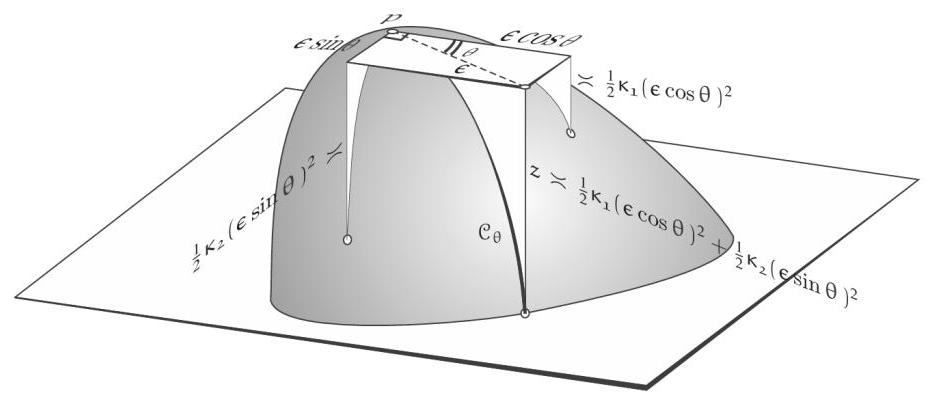
\includegraphics[width=0.7\textwidth]{fig/bo_d4vqblv7aajc73ft760g_11_283_240_931_400_0.jpg}
\end{center}
\hspace*{3em} 

Figure 6. The principal curvatures tell us how quickly the surface falls away - downwards in this figure from the tangent plane as we begin to travel in each of the two perpendicular principal directions. When we instead move a distance \(\epsilon\) within the tangent plane in a general direction \(\theta\) , the distance \(z\) that the surface falls away is simply the sum of the falls due to each of these two components separately.

Lemma 5 (Singular Value Decomposition (SVD))

\[
M = {R}_{\varphi } \circ  \sum  \circ  {R}_{-\theta }
\]

\begin{center}
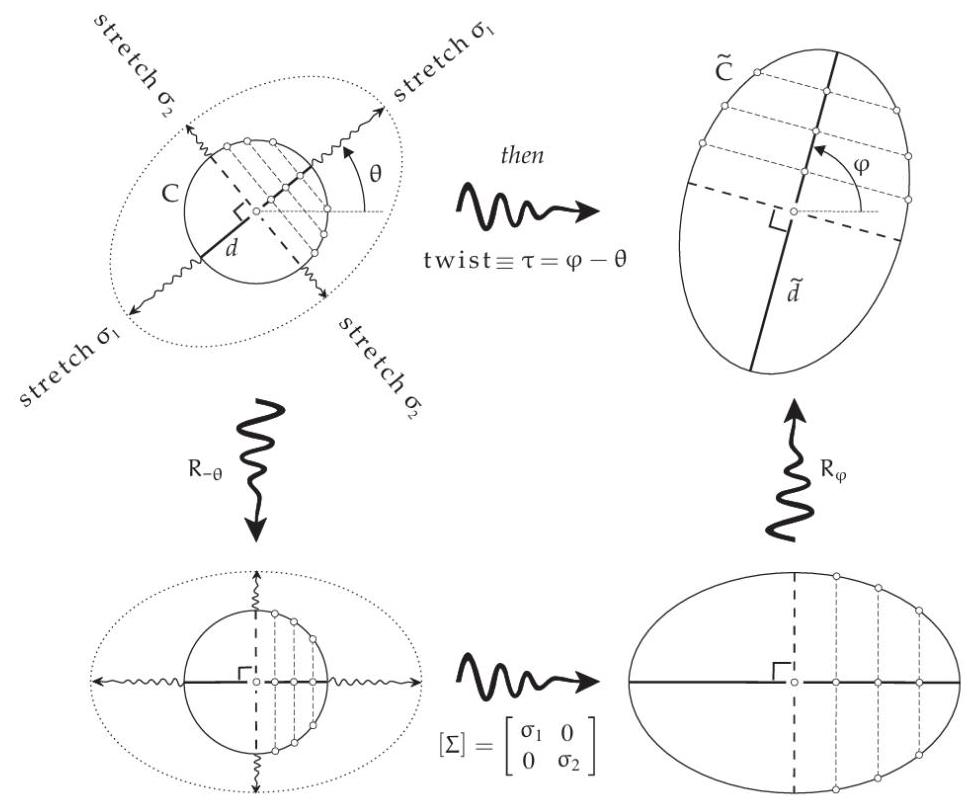
\includegraphics[width=0.7\textwidth]{fig/bo_d4vqblv7aajc73ft760g_11_266_1006_975_804_0.jpg}
\end{center}
\hspace*{3em} 

Figure 7. Singular Value Decomposition (SVD): The top half of the figure illustrates the effect, from left to right, of a general linear transformation \(M\) on an origin-centered circle. Preservation of midpoints enables us to prove that \(M\) is equivalent to two perpendicular stretches (by the "singular values" \({\sigma }_{1}\) and \({\sigma }_{2}\) ), followed by a rotation, which we call the twist \(\equiv  \tau\) ; here \(\tau  = \varphi  - \theta\) . The bottom half of the figure demonstrates that this SVD is equivalent to being able to write \(M = {R}_{\varphi } \circ  \sum  \circ  {R}_{-\theta }\) , where \(\sum\) stretches horizontally by \({\sigma }_{1}\) and vertically by \({\sigma }_{2}\) .

7 The Shape Operator \(\mathcal{S}\) is a geometric entity, independent of any particular choice of basis vectors, but the matrix \(\left\lbrack  \mathcal{S}\right\rbrack\) certainly does depend row his choice it's because \(\left\lbrack  \mathcal{S}\right\rbrack   = {\left\lbrack  \mathcal{S}\right\rbrack  }^{T}\) , which may relate to the self-adjoint property of \(\mathcal{S}\) .

Definition 33 (The general matrix of \(\mathcal{S}\) )

\({}^{7}\) Suppose that we choose an arbitrary orthonormal basis \(\left\{  {{E}_{1},{E}_{2}}\right\}\) , without first finding the principal directions and curvatures; how will the matrix look? While we may not yet know the principal directions, they certainly exist, so let us suppose that \(\left\{  {{e}_{1},{e}_{2}}\right\}\) are obtained by rotating \(\left\{  {{E}_{1},{E}_{2}}\right\}\) through some unknown angle \(\theta\) , then \({}^{8}\)

\[
\left\lbrack  \mathcal{S}\right\rbrack   = {R}_{\theta } \circ  \sum  \circ  {R}_{-\theta }
\]

\begin{center}
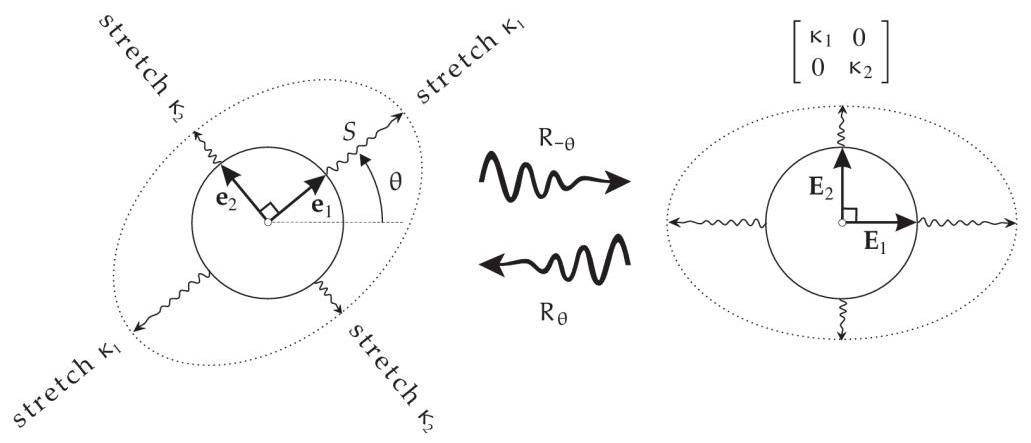
\includegraphics[width=0.8\textwidth]{fig/bo_d4vqblv7aajc73ft760g_12_248_553_1031_443_0.jpg}
\end{center}
\hspace*{3em} 

Figure 8. On the left, \(\mathcal{S}\) stretches the orthogonal principal directions by factors equal to the principal curvatures, deforming the unit circle into an ellipse aligned with the principal directions. This effect of \(\mathcal{S}\) is equivalent to first rotating by \(- \theta\) , producing the figure on the right, then stretching horizontally by \({\kappa }_{1}\) and vertically by \({\kappa }_{2}\) , then rotating back by \(\theta\) .

Definition 34

A point \(p \in  S\) is called

\begin{itemize}\relax
\item\relax umbilic (novel): if \({\kappa }_{1}\left( p\right)  = {\kappa }_{2}\left( p\right)\) , i.e. \({\kappa }_{p}\left( u\right)\) is independent of \(u\) , ex every point on the sphere.
\end{itemize}

\begin{itemize}\relax
\item\relax elliptic: if \({\kappa }_{1}\left( p\right)\) and \({\kappa }_{2}\left( p\right)\) have the same sign \(\left( {{\kappa }_{1} \neq  {\kappa }_{2}}\right)\)
\end{itemize}

\begin{itemize}\relax
\item\relax hyperbolic: if \({\kappa }_{1}\left( p\right)\) and \({\kappa }_{2}\left( p\right)\) have the opposite sign, which is saddle-like.
\end{itemize}

\begin{itemize}\relax
\item\relax parabolic: if \({\kappa }_{1}\left( p\right)  = 0\) or \({\kappa }_{2}\left( p\right)  = 0\) , ex cylinder.
\end{itemize}

\begin{center}
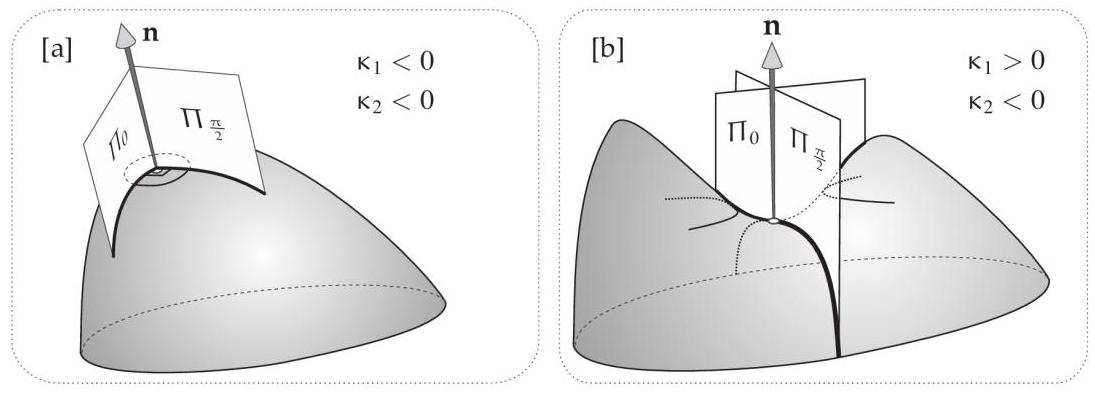
\includegraphics[width=0.8\textwidth]{fig/bo_d4vqblv7aajc73ft760g_12_206_1555_1095_393_0.jpg}
\end{center}
\hspace*{3em} 

Figure 9. [a] If \({\kappa }_{1}\) and \({\kappa }_{2}\) have the same sign then the surface locally resembles a hill, and a slice parallel to the tangent plane yields an ellipse (or misses the surface entirely). [b] If \({\kappa }_{1}\) and \({\kappa }_{2}\) have opposite sign then the surface locally resembles a saddle. A parallel slice above the tangent plane yields both branches of a hyperbola.

Definition 35 (Darboux frame)

A frame \({e}_{1},{e}_{2},{e}_{3}\) adapted to \(S\) is called the Darboux frame if \({e}_{1}\left( p\right)\) and \({e}_{2}\left( p\right)\) are the principle directions at \(p\) .

Definition 36 (Line of curvature)

A unit-speed curve \(c\) is called a line of curvature if \(\dot{c}\) is always a principal direction, e.g. \(\dot{c}\left( t\right)  = {u}_{1}\left( {c\left( t\right) }\right)\) .

\HRule

Theorem 10 (do Carmo 3.4.4, O'Neill,

Proposition 12

(The rate of change of the principal curvature)

\HRule

Away from umbilic points, a Darboux frame frame always exists.

\[
d{\kappa }_{1}\left( {e}_{2}\right)  = \left( {{\kappa }_{1} - {\kappa }_{2}}\right) {\omega }_{1}^{2}\left( {e}_{1}\right) \tag{10.1}
\]

\[
d{\kappa }_{2}\left( {e}_{1}\right)  = \left( {{\kappa }_{1} - {\kappa }_{2}}\right) {\omega }_{1}^{2}\left( {e}_{2}\right)
\]

Proof Suppose \(\left\{  {{e}_{1},{e}_{2},{e}_{3}}\right\}\) is a Darboux frame on \(S,\mathcal{S}{e}_{1} = {\kappa }_{1}{e}_{1},\mathcal{S}{e}_{2} = {\kappa }_{2}{e}_{2}\) . Hence

\[
I{I}_{ij} = {II}\left( {{e}_{i},{e}_{j}}\right)  = {e}_{i} \cdot  \mathcal{S}{e}_{j}
\]

Moreover,

\[
{\omega }_{1}^{3} = {\kappa }_{1}{\theta }^{1},\;{\omega }_{2}^{3} = {\kappa }_{2}{\theta }^{2} \tag{10.2}
\]

take \(d\) :

\[
d{\omega }_{1}^{3} = d{\kappa }_{1} \land  {\theta }^{1} + {\kappa }_{1}d{\theta }^{1}
\]

As

\[
d\left\lbrack  \omega \right\rbrack   = \left\lbrack  \omega \right\rbrack   \land  \left\lbrack  \omega \right\rbrack   \Rightarrow  d{\omega }_{1}^{3} = {\omega }_{1}^{2} \land  {\omega }_{2}^{3}
\]

\[
d\left\lbrack  \theta \right\rbrack   = \left\lbrack  \omega \right\rbrack   \land  \left\lbrack  \theta \right\rbrack   \Rightarrow  d{\theta }^{1} = {\omega }_{1}^{2} \land  {\theta }^{2} + {\omega }_{1}^{3} \land  {\theta }^{3} = {\omega }_{1}^{2} \land  {\theta }^{2}
\]

here we assume \({\theta }^{3} = 0\) , we have

\[
{\omega }_{1}^{2} \land  {\omega }_{2}^{3} = d{\kappa }_{1} \land  {\theta }^{1} + {\kappa }_{1}{\omega }_{1}^{2} \land  {\theta }^{2}
\]

substitute \({\omega }_{2}^{3}\) by equation (10.2), then

\[
d{\kappa }_{1} \land  {\theta }^{1} = {\omega }_{1}^{2} \land  {\omega }_{2}^{3} - {\kappa }_{1}{\omega }_{1}^{2} \land  {\theta }^{2}
\]

\[
= {\omega }_{1}^{2} \land  \left( {{\kappa }_{2}{\theta }^{2}}\right)  - {\kappa }_{1}{\omega }_{1}^{2} \land  {\theta }^{2} \tag{10.3}
\]

\[
= \left( {{\kappa }_{2} - {\kappa }_{1}}\right) {\omega }_{1}^{2} \land  {\theta }^{2}
\]

Apply basis \(\left( {{e}_{1},{e}_{2}}\right)\) to the above equation (10.3), we get

\[
- d{\kappa }_{1}\left( {e}_{2}\right)  = \left( {{\kappa }_{2} - {\kappa }_{1}}\right) {\omega }_{1}^{2}\left( {e}_{1}\right)
\]

i.e.

\[
d{\kappa }_{1}\left( {e}_{2}\right)  = \left( {{\kappa }_{1} - {\kappa }_{2}}\right) {\omega }_{1}^{2}\left( {e}_{1}\right)
\]

Similarly

\[
d{\kappa }_{2}\left( {e}_{1}\right)  = \left( {{\kappa }_{1} - {\kappa }_{2}}\right) {\omega }_{1}^{2}\left( {e}_{2}\right)
\]

Remark \({\omega }_{1}^{2}\) is measuring the change of principal curvature/directions.

\HRule

"In both these equations, \({\omega }_{1}^{2}\left( v\right)\) tells us how fast the principal directions are rotating within \(S\) as we move along the surface in the direction \(v\) . So, putting both equations into words, as we move off at right angles to a principal direction, the rate of change of that principal curvature is proportional to both the difference of the two principal curvatures, and to the rate at which the principal directions rotate."

Selected from Needham, Visual Differential Geometry and Forms: A Mathematical Drama in Five Acts, 38.6

\HRule

Gaussian curvature

The preceding subsection found the geometrical meaning of the eigenvalues and eigenvectors of the shape operator. Now we examine the determinant and trace of \(S\) , i.e. extract numbers from a matrix, independent of the basis. That is, apply a \(2 \times  2\) matrix to the shape operator.

Definition 37 (Gaussian and mean curvature) Example

\(\kappa \left( t\right)  = \det {\mathcal{S}}_{p} = {\kappa }_{1}\left( p\right)  \cdot  {\kappa }_{2}\left( p\right)\) is called the Gaussian curvature. And \(H\left( p\right)  = \frac{1}{2}\operatorname{tr}{\mathcal{S}}_{p} = \; \frac{1}{2}\left( {{\kappa }_{1}\left( p\right)  + {\kappa }_{2}\left( p\right) }\right)\) is called the mean curvature.

plane: \(\kappa  = 0 = H\) .

cylinder: \(\kappa  = 0,H \neq  0\) .

sphere of radius \(R : \kappa  = \frac{1}{{R}^{2}}\) .

Remark \(\kappa \left( p\right)  > 0, = 0, < 0 \Leftrightarrow  p\) is elliptic, parabolic, hyperbolic.

Proposition 13 (Characteristic polynomial of \({\mathcal{S}}_{p})\)

\[
\det \left( {{\mathcal{S}}_{p} - {\lambda Id}}\right)  = \left( {{\kappa }_{1} - \lambda }\right) \left( {{\kappa }_{2} - \lambda }\right)  = {\lambda }^{2} - {2H\lambda } + \kappa
\]

In particular, \({\kappa }_{1},{\kappa }_{2} = H \pm  \sqrt{{H}^{2} - \kappa }\) .

Proposition 14

Let \({e}_{1},{e}_{2},{e}_{3}\) be a moving frame adapted to \(S \in  {\mathbb{R}}^{3}\) with dual frame \({\theta }^{j}\) and connection forms \({\omega }_{i}^{j}\) , then

\[
d{\omega }_{2}^{1} = \kappa {\theta }^{1} \land  {\theta }^{2} \tag{11.1}
\]

\[
{\omega }_{1}^{3} \land  {\theta }^{2} + {\theta }^{1} \land  {\omega }_{2}^{3} = {2H}{\theta }^{1} \land  {\theta }^{2} \tag{11.2}
\]

Proof Recall \(I{I}_{ij} = {e}_{i} \cdot  {\mathcal{S}}_{p}{e}_{j}\) is the matrix expression of \({\mathcal{S}}_{p}\) , then

\[
\det \left( {I{I}_{ij}}\right)  = \kappa ,\;\operatorname{tr}I{I}_{ij} = {2H}
\]

thus

\[
d{\omega }_{2}^{1} =  - d{\omega }_{1}^{2} =  - {\omega }_{1}^{3} \land  {\omega }_{3}^{2} = {\omega }_{1}^{3} \land  {\omega }_{2}^{3}
\]

\[
= \left( {I{I}_{11}{\theta }^{1} + I{I}_{12}{\theta }^{2}}\right)  \land  \left( {I{I}_{21}{\theta }^{1} + I{I}_{22}{\theta }^{2}}\right)
\]

\[
= \left( {I{I}_{11}I{I}_{22} - I{I}_{12}I{I}_{21}}\right) {\theta }^{1} \land  {\theta }^{2}
\]

\[
= \det I{I}_{ij}{\theta }^{1} \land  {\theta }^{2}
\]

\[
= \kappa {\theta }^{1} \land  {\theta }^{2}
\]

and

\[
{\omega }_{1}^{3} \land  {\theta }^{2} + {\theta }^{1} \land  {\omega }_{2}^{3} = I{I}_{11}{\theta }^{1} \land  {\theta }^{2} + I{I}_{22}{\theta }^{1} \land  {\theta }^{2}
\]

\[
= {2H}{\theta }^{1} \land  {\theta }^{2}
\]

\({\omega }_{1}^{2}\) measures the rate of change of the frame \({e}_{1},{e}_{2}\) on \(S\) , and \(\kappa\) becomes kind of second order rate of change. Eq (11.1) depends only on \({e}_{1},{e}_{2}\) , which means \(\kappa\) only depends on the behavior of \({e}_{1},{e}_{2}\) . In contrast, according to eq (11.2), \({II},{\mathcal{S}}_{p},{\omega }_{1}^{3},{\omega }_{2}^{3}\) and \(H\) all depend on \({e}_{1},{e}_{2},{e}_{3}\) . The astonishing thing is \(\kappa  = {\kappa }_{1}{\kappa }_{2}\) is independent of \({e}_{3}\) .

To sum up, for a adapted frame \({e}_{1},{e}_{2},{e}_{3}\) with dual frame \({\theta }_{1},{\theta }_{2},{\theta }_{3}\) and connection forms \({\omega }_{i}^{j}\) , restricted to \(S\) (only on \({\mathrm{T}}_{p}S\) ), we have

\begin{itemize}\relax
\item\relax \({\theta }_{1},{\theta }_{2}\) are the dual frame of \({e}_{1}\left( p\right) ,{e}_{2}\left( p\right)  \in  {\mathrm{T}}_{p}S\)
\end{itemize}

\begin{itemize}\relax
\item\relax \({\omega }_{1}^{2}\) measures the rate of change of \({e}_{1},{e}_{2}\)
\end{itemize}

\begin{itemize}\relax
\item\relax \({\theta }_{3} = 0\)
\end{itemize}

\begin{itemize}\relax
\item\relax \({\omega }_{1}^{3},{\omega }_{2}^{3}\) describe the shape operator \({II}\)
\end{itemize}

\HRule

Theorem 11 (The six fundamental form equations of a surface)

\HRule

1st structure equations on \(S\)

\[
d{\theta }^{1} = {\omega }_{1}^{2} \land  {\theta }^{2}
\]

\[
d{\theta }^{2} = {\omega }_{2}^{1} \land  {\theta }^{1}
\]

Symmetry equation

\[
{\omega }_{1}^{3} \land  {\theta }^{1} + {\omega }_{2}^{3} \land  {\theta }^{2} = 0
\]

\[
{\omega }_{1}^{3} \land  {\theta }^{2} + {\omega }_{2}^{3} \land  {\theta }^{1} = {2H}{\theta }^{1} \land  {\theta }^{2}
\]

2nd structure equations on \(S\)

Gaussian equation

\[
d{\omega }_{1}^{2} =  - \kappa {\theta }^{1} \land  {\theta }^{2}
\]

Codazzi equations (change of shape operator)

\[
d{\omega }_{1}^{3} = {\omega }_{1}^{2} \land  {\omega }_{2}^{3}
\]

\[
d{\omega }_{2}^{3} = {\omega }_{2}^{1} \land  {\omega }_{1}^{3}
\]

Roughly speaking, intrinsic properties can be measured by inhibitions living on \(S( =\) ant perspective); extrinsic properties depend on how the surface \(S\) is realized as a subset of \({\mathbb{R}}^{3}\) (= space view).

Next we want to see how do frame properties transform as we change our surface. Suppose \(F : S\left( { \subseteq  {\mathbb{R}}^{3}}\right)  \rightarrow  \bar{S}\left( { \subseteq  {\mathbb{R}}^{3}}\right)\) , and we want to use \(F\) to compare objects living on \(\bar{S}\) with the objects on \(S\) .

Definition 38 (Pushforward and Pullback) pushforward: objects on \(S \rightarrow\) objects on \(\bar{S}\) .

pullback: objects living on \(\bar{S}\) induce something living on \(S\) .

Example (Pushforward of curves) If \(c : I \rightarrow  S\) , then the pushforward of \(c\) via \(F\) is the curve in \(\bar{S}\) .

\[
{c}_{F} = F \circ  c : I \rightarrow  \bar{S}
\]

i.e.

\[
{c}_{F}\left( t\right)  = F\left( {c\left( t\right) }\right)
\]

Example

(Pushforward of tangent vectors) If \(v \in  {\mathrm{T}}_{p}S\) , represented by a curve \(c : I \rightarrow  S\) , then the pushforward of \(v\) is the tangent vector \(w \in  {T}_{F\left( p\right) }\bar{S}\) represented by the curve \({c}_{F} = F \circ  c\) , i.e.

\[
w = {\left. \frac{\mathrm{d}}{\mathrm{d}t}\right| }_{t = 0}F\left( {c\left( t\right) }\right)  = {\mathrm{T}}_{p}F\left( {{\left. \frac{\mathrm{d}}{\mathrm{d}t}\right| }_{t = 0}c\left( t\right) }\right)  = {\mathrm{T}}_{p}F\left( v\right)
\]

therefore, this pushforward is just the derivative \({\mathrm{T}}_{p}F : {\mathrm{T}}_{p}S \rightarrow  {T}_{F\left( p\right) }\bar{S}\) .

Example

(Pullback of a 1-form) If \(\alpha\) is a 1-form on \(\bar{S}\) , then the pullback of \(\alpha\) by \(F\) is the 1-form \(\beta\) defined by

\[
{\beta }_{p}\left( v\right)  = {\alpha }_{F\left( p\right) }\left( {{\mathrm{T}}_{p}F\left( v\right) }\right)  \in  \mathbb{R},p \in  S,v \in  {\mathrm{T}}_{p}S,{\mathrm{\;T}}_{p}F\left( v\right)  \in  {T}_{F\left( p\right) }\bar{S}
\]

| Moreover, the 1-form \(\beta\) is usually written as \(\beta  = {F}^{ * }\alpha\) .

Example

(Pullback of bilinear forms) If \({\alpha }_{\bar{p}} : {T}_{\bar{p}}\bar{S} \times  {T}_{\bar{p}}\bar{S} \rightarrow  \mathbb{R}\) is a (smooth) family of bilinear forms on \(\bar{S}\) , then the pullback \({\left( {F}^{ * }\alpha \right) }_{p} : {\mathrm{T}}_{p}S \times  {\mathrm{T}}_{p}S \rightarrow  \mathbb{R}\) is defined by

\[
{\left( {F}^{ * }\alpha \right) }_{p}\left( {v,w}\right)  = {\alpha }_{F\left( p\right) }\left( {{\mathrm{T}}_{p}F\left( v\right) ,{\mathrm{T}}_{p}F\left( w\right) }\right)  \in  \mathbb{R},\;{\mathrm{T}}_{p}F\left( v\right) ,{\mathrm{T}}_{p}F\left( w\right)  \in  {T}_{F\left( p\right) }\bar{S}
\]

which is a family of bilinear forms on \(S\) , with the same symmetries as \(\alpha\) .

Example \(\phi  : {\mathbb{R}}^{2} \supseteq  U \rightarrow  S\) is a chart on \(S\) , then

\[
{\phi }^{ * }{II} = I{I}^{\phi }
\]

\[
{\phi }^{ * }\alpha  = {\alpha }^{\phi }
\]

if \(\alpha\) is a 1 or 2 form.

Proposition 15 If \(\alpha\) and \(\beta\) are 1-forms on \(\bar{S}\) , then

\[
{F}^{ * }\left( {\alpha  \land  \beta }\right)  = \left( {{F}^{ * }\alpha }\right)  \land  \left( {{F}^{ * }\beta }\right)
\]

\[
d\left( {{F}^{ * }\alpha }\right)  = {F}^{ * }\left( {d\alpha }\right)
\]

Proof

\[
{\left( {F}^{ * }\left( \alpha  \land  \beta \right) \right) }_{p}\left( {v,w}\right)  = {\left( \alpha  \land  \beta \right) }_{F\left( p\right) }\left( {{\mathrm{T}}_{p}F\left( v\right) ,{\mathrm{T}}_{p}F\left( w\right) }\right)
\]

\[
= {\alpha }_{F\left( p\right) }\left( {{\mathrm{T}}_{p}F\left( v\right) }\right)  \cdot  {\beta }_{F\left( p\right) }\left( {{\mathrm{T}}_{p}F\left( w\right) }\right)  - {\alpha }_{F\left( p\right) }\left( {{\mathrm{T}}_{p}F\left( w\right) }\right)  \cdot  {\beta }_{F\left( p\right) }\left( {{\mathrm{T}}_{p}F\left( v\right) }\right)
\]

\[
= \left( {{F}^{ * }{\alpha }_{p}}\right) \left( v\right)  \cdot  \left( {{F}^{ * }{\beta }_{p}}\right) \left( w\right)  - \left( {{F}^{ * }{\alpha }_{p}}\right) \left( w\right)  \cdot  \left( {{F}^{ * }{\beta }_{p}}\right) \left( v\right)
\]

\[
= {\left( \left( {F}^{ * }\alpha \right)  \land  \left( {F}^{ * }\beta \right) \right) }_{p}\left( {v,w}\right)
\]

Let \(\phi  : U \rightarrow  S\) be a chart on \(S\) , then

\[
{\left( d\left( {F}^{ * }\alpha \right) \right) }_{\phi \left( {x,y}\right) }\left( {{T}_{x,y}\phi \left( {\partial x}\right) ,{T}_{x,y}\phi \left( {\partial y}\right) }\right)
\]

\[
= \frac{\partial }{\partial x}\left( {{\left( {F}^{ * }\alpha \right) }_{\phi \left( {x,y}\right) }{T}_{x,y}\phi \left( {\partial y}\right) }\right)  - \frac{\partial }{\partial y}\left( {{\left( {F}^{ * }\alpha \right) }_{\phi \left( {x,y}\right) }{T}_{x,y}\phi \left( {\partial x}\right) }\right)
\]

\[
= \frac{\partial }{\partial x}\left( {{\alpha }_{F\left( {\phi \left( {x,y}\right) }\right) }{T}_{\phi \left( {x,y}\right) }F\left( {{T}_{x,y}\phi \left( {\partial y}\right) }\right) }\right)  - \frac{\partial }{\partial y}\left( {{\alpha }_{F\left( {\phi \left( {x,y}\right) }\right) }{T}_{\phi \left( {x,y}\right) }F\left( {{T}_{x,y}\phi \left( {\partial x}\right) }\right) }\right)
\]

\[
= \frac{\partial }{\partial x}\left( {{\alpha }_{F\left( {\phi \left( {x,y}\right) }\right) }{T}_{x,y}\left( {F \circ  \phi }\right) \left( {\partial y}\right) }\right)  - \frac{\partial }{\partial y}\left( {{\alpha }_{F\left( {\phi \left( {x,y}\right) }\right) }{T}_{x,y}\left( {F \circ  \phi }\right) \left( {\partial x}\right) }\right)
\]

\[
= {\left( d\alpha \right) }_{F\left( {\phi \left( {x,y}\right) }\right) }\left( {{T}_{x,y}\left( {F \circ  \phi }\right) \left( {\partial x}\right) ,{T}_{x,y}\left( {F \circ  \phi }\right) \left( {\partial y}\right) }\right)
\]

\[
= {\left( {F}^{ * }\left( d\alpha \right) \right) }_{\phi \left( {x,y}\right) }\left( {{T}_{x,y}\phi \left( {\partial x}\right) ,{T}_{x,y}\phi \left( {\partial y}\right) }\right)
\]

Definition 39 (Isometry of surfaces) An isometry of surfaces \(S\) and \(\bar{S}\) is a bijective map \(F : S \rightarrow  \bar{S}\) that preserves the inner

product of tangent vectors:

\[
v \cdot  w = {\mathrm{T}}_{p}F\left( v\right)  \cdot  {\mathrm{T}}_{p}F\left( w\right) ,\;\forall v,w \in  {\mathrm{T}}_{p}S
\]

i.e.

\[
{F}^{ * }\bar{I} = I
\]

Definition 40 (Local isometry)

Local isometry is a map \(F : S \rightarrow  \bar{S}\) such that every point \(p \in  S\) has some neighborhood \(U \subseteq  S\) such that \(F : S \supseteq  U \rightarrow  F\left( U\right)  \subseteq  \bar{S}\) is a isometry.

According to definition, (local) isometries preserve the length of tangent vectors, but does it also preserve the distance of two points at the surface?

Definition 41 (Distance on the surface) The distance between \(p,q \in  S\) is

\[
d\left( {p,q}\right)  = \inf \left( c\right) ,\text{ with }c\left( 0\right)  = p,c\left( 1\right)  = q
\]

Proposition 16 For every isometry \(F\)

\[
d\left( {p,q}\right)  = d\left( {F\left( p\right) ,F\left( q\right) }\right) ,\;\forall p,q \in  S
\]

Proof \({\mathrm{T}}_{p}F : {\mathrm{T}}_{p}S \rightarrow  {\mathrm{T}}_{p}\bar{S}\) preserves the length of vectors, thus

\[
L\left( c\right)  = L\left( {F \circ  c}\right)  = {\int }_{0}^{1}\begin{Vmatrix}{\frac{\mathrm{d}}{\mathrm{d}t}F\left( {c\left( t\right) }\right) }\end{Vmatrix}\mathrm{d}t
\]

Theorem 12 (Gauss Theorema Egregium, 1827, "Remarkable Theorem")

The Gauss curvature \(\kappa\) of a surface \(S\) only depends on the first fundamental form \(I\) on \(S\) , and it’s invariant under local isometries \(F : S \rightarrow  \bar{S}\) , i.e.

\(\kappa \left( p\right)  = \overline{\kappa }\left( {F\left( p\right) }\right) ,\;\forall p \in  S,\) where \(\overline{\kappa } : \bar{S} \rightarrow  \mathbb{R}\) gauss curvature of \(\bar{S}\)

Idea of the proof is

\begin{itemize}\relax
\item\relax Use the structure equation
\end{itemize}

\[
d{\theta }^{1} = {\omega }_{1}^{2} \land  {\theta }^{2}
\]

\[
d{\theta }^{2} = {\omega }_{2}^{1} \land  {\theta }^{1}
\]

to say that \({\omega }_{1}^{2} =  - {\omega }_{2}^{1}\) is uniquely defined by \({\theta }^{1},{\theta }^{2}\) , and thus only depends on \(I\) .

\begin{itemize}\relax
\item\relax Use the Gauss equation \(d{\omega }_{1}^{2} =  - \kappa {\theta }^{1} \land  {\theta }^{2}\) to conclude that \(\kappa\) depends only on \(I\) .
\end{itemize}

Lemma 6

\begin{itemize}\relax
\item\relax If \(\left( {{e}_{1},{e}_{2},{e}_{3}}\right)\) is a frame on \({\mathbb{R}}^{3}\) adapted to \(S\) , then \({e}_{1}\left( p\right)\) and \({e}_{2}\left( p\right)\) form an orthonormal basis of \({\mathrm{T}}_{p}S\) with respect to \(S\) , because \(I\left( {{e}_{i},{e}_{j}}\right)  = {e}_{i} \cdot  {e}_{j}\) .
\end{itemize}

\begin{itemize}\relax
\item\relax Conversely, if \({e}_{1},{e}_{2}\) are vector fields on \(S\) forming an ONB of \({\mathrm{T}}_{p}S,\forall p \in  S\) , then they can be extended to a frame \({e}_{1},{e}_{2},{e}_{3}\) on \({\mathbb{R}}^{3}\) adapted to \(S\) .
\end{itemize}

Lemma 7 There exists exactly one 1-form \(\alpha\) on \(S\) satisfying

\[
d{\theta }^{1} = \alpha  \land  {\theta }^{2}\;\text{ and }\;d{\theta }^{2} =  - \alpha  \land  {\theta }^{1} \tag{11.3}
\]

Proof Apply \({e}_{1},{e}_{2}\) to the equations

\[
d{\theta }^{1}\left( {{e}_{1},{e}_{2}}\right)  = \alpha  \land  {\theta }^{2}\left( {{e}_{1},{e}_{2}}\right)  = \alpha \left( {e}_{1}\right) {\theta }^{2}\left( {e}_{2}\right)  - 0 = \alpha \left( {e}_{1}\right)
\]

\[
d{\theta }^{2}\left( {{e}_{1},{e}_{2}}\right)  =  - \alpha  \land  {\theta }^{1}\left( {{e}_{1},{e}_{2}}\right)  = 0 + \alpha \left( {e}_{2}\right) {\theta }^{1}\left( {e}_{1}\right)  = \alpha \left( {e}_{2}\right)
\]

\(\alpha\) is uniquely defined by these equations, and the unique 1-form satisfying (11.3) is called the connection form associated with \({e}_{1},{e}_{2}\) , written as \(\alpha  = {\omega }_{1}^{2}\) . That is, \({\omega }_{1}^{2}\) on \(S\) only depends on \({e}_{1},{e}_{2}\) , and thus only \(I\) , not on \({II}/\mathcal{S}\) .

Lemma 8 There exists a unique function \(\kappa\) on \(S\) such that

\[
d{\omega }_{1}^{2} = \kappa {\theta }^{1} \land  {\theta }^{2}
\]

where \({\omega }_{1}^{2}\) is the connection of the tangent frame \({e}_{1},{e}_{2}\) .

Proof Evaluate the equation on \({e}_{1},{e}_{2}\)

\[
d{\omega }_{1}^{2}\left( {{e}_{1},{e}_{2}}\right)  = \kappa {\theta }^{1} \land  {\theta }^{2}\left( {{e}_{1},{e}_{2}}\right)  = \kappa
\]

which means \(\kappa\) only depends on the tangent plane \({e}_{1},{e}_{2}\) .

\HRule

Lemma 9 (Behavior of \({e}_{1},{e}_{2},{\theta }^{1},{\theta }^{2}\) and \({\omega }_{1}^{2}\) under isometries)

\HRule

\(F : S \rightarrow  \bar{S}\) isometry. Let \({e}_{1},{e}_{2}\) be a tangent plane on \(S\) , with dual frame \({\theta }^{1},{\theta }^{2}\) and connection form \({\omega }_{1}^{2}\) , then

1. \({\bar{e}}_{1}\left( \bar{p}\right)  = {\mathrm{T}}_{p}F\left( {{e}_{1}\left( p\right) }\right) ,{\bar{e}}_{2}\left( \bar{p}\right)  = {\mathrm{T}}_{p}F\left( {{e}_{2}\left( p\right) }\right) \left( {\bar{p} = F\left( p\right) }\right)\) , are tangent frames on \(\bar{S}\)

2. The dual tangent frame \({\overline{\theta }}^{1},{\overline{\theta }}^{2}\) on \(\bar{S}\) associated with \({\bar{e}}_{1},{\bar{e}}_{2}\) is uniquely defined by

\[
{F}^{ * }{\overline{\theta }}^{1} = {\theta }^{1},\;{F}^{ * }{\overline{\theta }}^{2} = {\theta }^{2}
\]

3. The connection form \({\overline{\omega }}_{1}^{2}\) on \(\bar{S}\) associated with \({\bar{e}}_{1},{\bar{e}}_{2}\) is uniquely defined by

\[
{F}^{ * }{\overline{\omega }}_{1}^{2} = {\omega }_{1}^{2}
\]

Proof 1.

\[
{\bar{I}}_{F\left( p\right) }\left( {{\bar{e}}_{i}\left( \bar{p}\right) ,{\bar{e}}_{j}\left( \bar{p}\right) }\right)  = {\bar{I}}_{F\left( p\right) }\left( {{\mathrm{T}}_{p}F\left( {{e}_{i}\left( p\right) }\right) ,{\mathrm{T}}_{p}F\left( {{e}_{j}\left( p\right) }\right) }\right)
\]

\[
= \left( {{F}^{ * }\bar{I}}\right) \left( {{e}_{i}\left( p\right) ,{e}_{j}\left( p\right) }\right)
\]

\[
= I\left( {{e}_{i}\left( p\right) ,{e}_{j}\left( p\right) }\right)
\]

which means \({\bar{e}}_{1},{\bar{e}}_{2}\) are orthonormal with respect to \(\bar{I}\) .

2. Let’s check \({F}^{ * }{\overline{\theta }}^{1} = {\theta }^{1}\) on the basis \({e}_{1},{e}_{2}\)

\[
{\left( {F}^{ * }{\overline{\theta }}^{1}\right) }_{p}\left( {e}_{1}\right)  = {\overline{\theta }}_{F\left( p\right) }^{1}\left( {{\mathrm{\;T}}_{p}F\left( {e}_{1}\right) }\right)  = {\overline{\theta }}_{F\left( p\right) }^{1}{\bar{e}}_{1}\left( \bar{p}\right)  = 1
\]

\[
{\left( {F}^{ * }{\overline{\theta }}^{1}\right) }_{p}\left( {e}_{2}\right)  = {\overline{\theta }}_{F\left( p\right) }^{1}\left( {{\mathrm{\;T}}_{p}F\left( {e}_{2}\right) }\right)  = {\overline{\theta }}_{F\left( p\right) }^{1}{\bar{e}}_{2}\left( \bar{p}\right)  = 0
\]

therefore

\[
{F}^{ * }{\overline{\theta }}^{1} = {\theta }^{1}
\]

and similarly for \({F}^{ * }{\overline{\theta }}^{2} = {\theta }^{2}\)

3. Recall for 1-forms \(\alpha ,\beta\) on \(\bar{S}\)

\[
{F}^{ * }\left( {\alpha  \land  \beta }\right)  = \left( {{F}^{ * }\alpha }\right)  \land  \left( {{F}^{ * }\beta }\right)
\]

\[
d\left( {{F}^{ * }\alpha }\right)  = {F}^{ * }\left( {d\alpha }\right)
\]

we have

\[
{F}^{ * }\left( {d{\overline{\theta }}^{1}}\right)  = d\left( {{F}^{ * }{\overline{\theta }}^{1}}\right)  = d{\theta }^{1}
\]

\[
{F}^{ * }\left( {d{\overline{\theta }}^{1}}\right)  = {F}^{ * }\left( {{\overline{\omega }}_{1}^{2} \land  {\overline{\theta }}^{2}}\right)  = \left( {{F}^{ * }{\overline{\omega }}_{1}^{2}}\right)  \land  \left( {{F}^{ * }{\overline{\theta }}^{2}}\right)  = \left( {{F}^{ * }{\overline{\omega }}_{1}^{2}}\right)  \land  {\theta }^{2}
\]

therefore

\[
d{\theta }^{1} = \left( {{F}^{ * }{\overline{\omega }}_{1}^{2}}\right)  \land  {\theta }^{2}
\]

and similarly

\[
d{\theta }^{2} =  - \left( {{F}^{ * }{\overline{\omega }}_{1}^{2}}\right)  \land  {\theta }^{1}
\]

thus

\[
{F}^{ * }{\overline{\omega }}_{1}^{2} = {\omega }_{1}^{2}
\]

Proof (Proof of the Gauss theorem)

\[
d{\overline{\omega }}_{1}^{2} =  - \overline{\kappa }{\overline{\theta }}^{1} \land  {\overline{\theta }}^{2}
\]

pull back by \({F}^{ * }\)

LHS \(\;{F}^{ * }\left( {d{\overline{\omega }}_{1}^{2}}\right)  = d\left( {{F}^{ * }{\overline{\omega }}_{1}^{2}}\right)  = d{\omega }_{1}^{2} =  - \kappa {\theta }^{1} \land  {\theta }^{2}\)

RHS \(\;{F}^{ * }\left( {-\overline{\kappa }{\overline{\theta }}^{1} \land  {\overline{\theta }}^{2}}\right)  = \left( {-\overline{\kappa } \circ  F}\right) {F}^{ * }\left( {{\overline{\theta }}^{1} \land  {\overline{\theta }}^{2}}\right)  =  - \overline{\kappa } \circ  F\left( {{F}^{ * }{\overline{\theta }}^{1}}\right)  \land  \left( {{F}^{ * }{\overline{\theta }}^{2}}\right)  =  - \overline{\kappa } \circ  F{\theta }^{1} \land  {\theta }^{2}\)

therefore

\[
- \kappa {\theta }^{1} \land  {\theta }^{2} =  - \overline{\kappa } \circ  F{\theta }^{1} \land  {\theta }^{2}
\]

Apply \({e}_{1},{e}_{2}\) to this equation, we have

\[
\kappa  = \overline{\kappa } \circ  F
\]

As we get the Remarkable Theorem, we wonder if we can reconstruct surfaces from curvature. The answer is in general no, but in some situations yes.

Theorem 13 (Reconstruct surfaces from curvature)

Let \(S \subseteq  {\mathbb{R}}^{3}\) surface such that every two points on \(S\) can be connected by a path in \(S\) and every point is an umbillic point, then \(S\) has constant Gaussian curvature \(\kappa  \geq  0\) , and

\begin{itemize}\relax
\item\relax If \(\kappa  = 0\) , then \(S\) is point of the plain
\end{itemize}

\begin{itemize}\relax
\item\relax If \(\kappa  > 0\) , then \(S\) is point of the sphere of radius \(\frac{1}{\sqrt{\kappa }}\)
\end{itemize}

Proof Assume \({e}_{1},{e}_{2},{e}_{3}\) an frame adapted to \(S\) . As every point is umbillic

\[
\mathcal{S}{e}_{1} = \kappa {e}_{1},\;\mathcal{S}{e}_{2} = \kappa {e}_{2}
\]

thus \({e}_{1},{e}_{2},{e}_{3}\) is a Darboux frame. According to equation (10.1), we have

\[
{d\kappa }\left( {e}_{1}\right)  = 0 = {d\kappa }\left( {e}_{2}\right)
\]

Theorem 14

If \(S\) is a compact surface in \({\mathbb{R}}^{3}\) with constant Guassian curvature \(\kappa  > 0\) , then \(S\) is the sphere of radius \(\frac{1}{\sqrt{\kappa }}\) .

Geodesics: parallel transport

\HRule

Proposition 17 (Geodesics in plane)

\HRule

In plane, the following are equivalent for a curve \(c\left( t\right)\)

1. \(c\left( t\right)\) is a straight line

2. curvature of \(c\) is zero, i.e. \(\ddot{c} = 0\)

3. \(\dot{c}\left( t\right)\) are parallel vectors for all \(t\)

4. extrema of the length functional \(( =\) is the shortest path between two points)

Next we consider the geodesics on the surface. Let \(c\) be a curve in \(S\) of constant speed \(v = \left| {\dot{c}\left( t\right) }\right|\) . Consider a frame \({e}_{1},{e}_{2},{e}_{3}\) a adapted frame satisfying \({e}_{1}\left( {c\left( t\right) }\right)  = \frac{\dot{c}\left( t\right) }{v}\) . Since \(\ddot{c} \cdot  \dot{c} = 0\) , there exists faculties \({\kappa }_{g}\left( t\right)\) and \({\kappa }_{n}\left( t\right)\) such that

\[
\frac{\ddot{c}\left( t\right) }{{v}^{2}} = {\kappa }_{g}\left( t\right) {e}_{2}\left( {c\left( t\right) }\right)  + {\kappa }_{n}\left( t\right) {e}_{3}\left( {c\left( t\right) }\right)
\]

curvature of curve

\[
\kappa \left( t\right)  = \frac{\parallel \ddot{c}\left( t\right) \parallel }{{v}^{2}} = \sqrt{{\kappa }_{g}^{2}\left( t\right)  + {\kappa }_{n}^{2}\left( t\right) }
\]

Also

\[
\frac{\ddot{c}\left( t\right) }{v} = \frac{\mathrm{d}}{\mathrm{d}t}\left( \frac{\dot{c}\left( t\right) }{v}\right)  = \frac{\mathrm{d}}{\mathrm{d}t}\left( {{e}_{1}\left( {c\left( t\right) }\right) }\right)  = {T}_{c\left( t\right) }{e}_{1}\left( {\dot{c}\left( t\right) }\right)
\]

\[
= {\omega }_{1}^{2}\left( {\dot{c}\left( t\right) }\right) {e}_{2}\left( {c\left( t\right) }\right)  + {\omega }_{1}^{3}\left( {\dot{c}\left( t\right) }\right) {e}_{3}\left( {c\left( t\right) }\right)
\]

\HRule

\({}^{9}\) Meusnier realized in 1779 that the surface forces all such curves to bend by the same amount: \({\kappa }_{n}\) is independent of the specific curve c. Suppose the curves are unit-speed, then

\[
{\kappa }_{n}\left( t\right)  = N \cdot  {e}_{3}
\]

\[
= \dot{T} \cdot  n
\]

\[
= T \cdot  \dot{n}
\]

But \(\dot{n}\) is the rate of change of the surface normal in the \(T\) direction, which is independent of the curves.

\HRule

therefore \({}^{9}\)

\[
{\kappa }_{g}\left( t\right)  = {\omega }_{1}^{2}\left( \frac{\dot{c}\left( t\right) }{v}\right) \;\text{ and }\;{\kappa }_{n}\left( t\right)  = {\omega }_{1}^{3}\left( \frac{\dot{c}\left( t\right) }{v}\right)
\]

\begin{center}
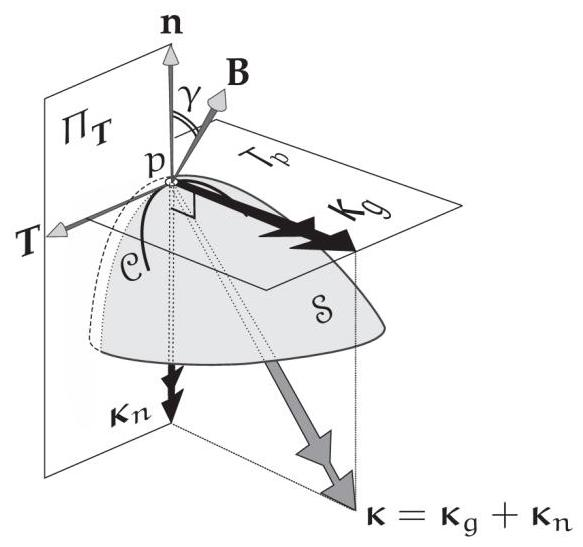
\includegraphics[width=0.4\textwidth]{fig/bo_d4vqblv7aajc73ft760g_20_470_1423_583_547_0.jpg}
\end{center}
\hspace*{3em} 

Figure 10. The curve acceleration \(\kappa\) can be decomposed into the geodesic curvature vector \({\kappa }_{g}\) tangent to the surface, and the normal curvature vector \({\kappa }_{n}\) perpendicular to the surface: \(\kappa  = {\kappa }_{g} + {\kappa }_{n}\)

\HRule

Definition 42 (Geodesic on the surface)

\HRule

A curve \(c\) with constant speed in \(S\) is called a geodesic if any of the following equiv properties hold:

1. \({\kappa }_{g}\left( t\right)  = 0\) ("intrinsically straight")

2. \(\ddot{c}\left( t\right)\) is completely in the normal direction

3. \({\omega }_{1}^{2}\left( {\dot{c}\left( t\right) }\right)  = 0\) , i.e. parallel transport (this section)

4. shortest length (next section)

Example

\(S =\) plane \({\mathbb{R}}^{2}\) in \({\mathbb{R}}^{3},c\left( t\right)  : I \rightarrow  {\mathbb{R}}^{2},\dot{c}\left( t\right)\) is normal (z-axis) iff \(\ddot{c}\left( t\right)  = 0\) , i.e. geodesics in \({\mathbb{R}}^{2}\) are just straight lines.

Example

\(S =\) sphere, a great circle is the intrinsic of the sphere with a plane through the origin. If we parametric such a great circle to have constant speed, then it is a geodesic, since its acceleration is purely pointing to the center (=normal).

In the plane, geodesics are exactly those curves with parallel tangent vectors. The question is, what is the notion of "parallel" on a surface.

\begin{center}
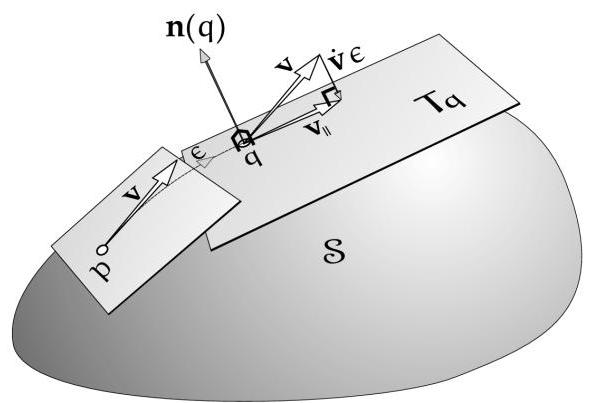
\includegraphics[width=0.4\textwidth]{fig/bo_d4vqblv7aajc73ft760g_21_465_912_591_403_0.jpg}
\end{center}
\hspace*{3em} 

Figure 11. Constructing a Geodesic via Parallel Transport. Launch a particle from \(p\) with velocity \(v\) , and define \(G\) to be the curve obtained by parallel-transporting \(v\) along itself, so that the new velocity at the neighboring point \(q\) is \({v}_{\left| \right| }\) . Then the acceleration \(\dot{v}\) is given by \(\dot{v}\epsilon  = {v}_{\mid  \mid  } - v\) . But then \(\dot{v} \propto  n\) , and therefore \(G\) is geodesic.

\HRule

Definition 43 (Vector field along curve)

\HRule

Let \(c : I \rightarrow  S\) be a curve. A vector field along \(c\) is a smooth map \(X : I \rightarrow  {\mathbb{R}}^{3}\) such that \(X\left( t\right)  \in  {T}_{c\left( t\right) }S\) for all \(t \in  I\) .

According to the definition, \(X\left( t\right)  = \dot{c}\left( t\right)\) is a vector field along \(c\) . The derivative of \(X\) , is a map \(\frac{\mathrm{d}}{\mathrm{d}t}X : I \rightarrow  {\mathbb{R}}^{3}\) , but \(\frac{\mathrm{d}}{\mathrm{d}t}X\) is usually not tangent to \(S\) . The idea to handle this is to decompose \(\frac{\mathrm{d}}{\mathrm{d}t}X\) into part that is tangent to \(S\) and another part that is normal.

For this purpose, choose a adapted frame \({e}_{1},{e}_{2},{e}_{3}\) on \(S\) , then

\[
X\left( t\right)  = {f}_{1}\left( t\right) {e}_{1}\left( {c\left( t\right) }\right)  + {f}_{2}\left( t\right) {e}_{2}\left( {c\left( t\right) }\right)
\]

for some smooth function \({f}_{1},{f}_{2} : I \rightarrow  \mathbb{R}\) , thus

\[
\frac{d}{dt}X\left( t\right)  = \left( {{\dot{f}}_{1}\left( t\right)  + {f}_{2}\left( t\right) {\omega }_{2}^{1}\left( {\dot{c}\left( t\right) }\right) }\right) {e}_{1}\left( {c\left( t\right) }\right)  + \left( {{\dot{f}}_{2}\left( t\right)  + {f}_{1}\left( t\right) {\omega }_{1}^{2}\left( {\dot{c}\left( t\right) }\right) }\right) {e}_{2}\left( {c\left( t\right) }\right)  +
\]

\[
\left( {{f}_{1}\left( t\right) {\omega }_{1}^{3}\left( {\dot{c}\left( t\right) }\right)  + {f}_{2}\left( t\right) {\omega }_{2}^{3}\left( {\dot{c}\left( t\right) }\right) }\right) {e}_{3}\left( {c\left( t\right) }\right)
\]

\HRule

Definition 44 (For the tangent part, covariant derivative)

\HRule

Let \({e}_{1},{e}_{2},{e}_{3}\) be a frame and \(X\left( t\right)  = {f}_{1}\left( t\right) {e}_{1}\left( {c\left( t\right) }\right)  + {f}_{2}\left( t\right) {e}_{2}\left( {c\left( t\right) }\right)\) be a vector field along the curve \(c\) , then covariant derivative of \(X\) is the vector field along \(c\) defined by

\[
\frac{\nabla }{dt}X\left( t\right)  = \left( {{\dot{f}}_{1} + {f}_{2}{\omega }_{2}^{1}\left( \dot{c}\right) }\right) {e}_{1}\left( {c\left( t\right) }\right)  + \left( {{\dot{f}}_{2} + {f}_{1}{\omega }_{1}^{2}\left( \dot{c}\right) }\right) {e}_{2}\left( {c\left( t\right) }\right)
\]

Note that \(\frac{\nabla }{dt}\) depends only on \({\omega }_{1}^{2}\) , is the "intrinsic derivative of \({X}^{\prime \prime }\) .

\begin{center}
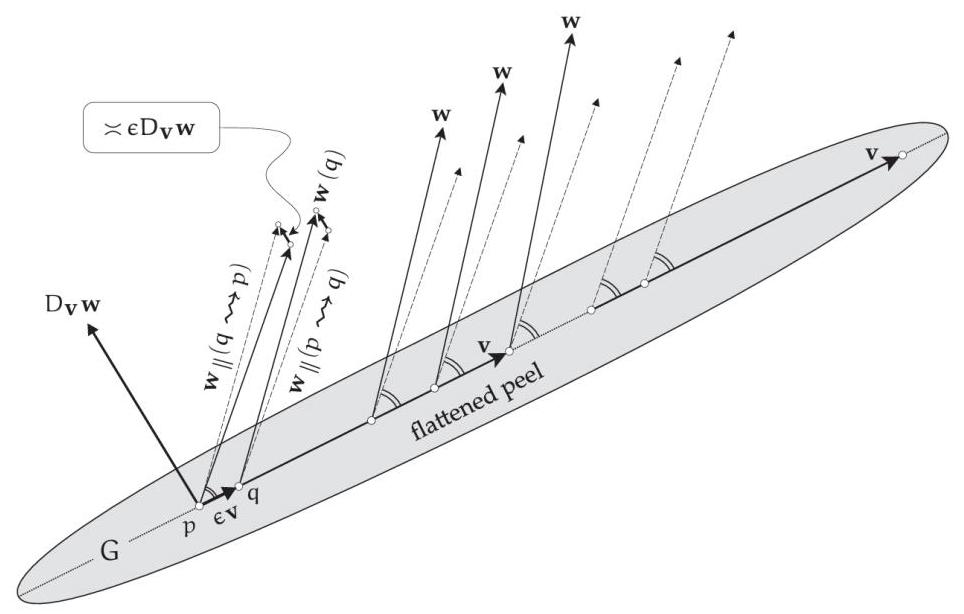
\includegraphics[width=0.7\textwidth]{fig/bo_d4vqblv7aajc73ft760g_22_294_598_964_614_0.jpg}
\end{center}
\hspace*{3em} 

Figure 12. The Intrinsic ("Covariant") Derivative, \({D}_{v}w\) , which measures the intrinsic rate of change of \(w\) along \(v\) , is especially easy to visualize if \(v\) is the velocity of a geodesic \(G\) , for then the trip of peel surrounding \(G\) flattens into a straight line, and parallel transport of \({w}_{\left| \right| }\) within the surface becomes ordinary Euclidean parallel transport within the plane.

Definition 45 (For the normal part) Consider

\[
\mathcal{S}\left( {\dot{c}\left( t\right) }\right)  = {\omega }_{1}^{3}\left( {\dot{c}\left( t\right) }\right) {e}_{1} + {\omega }_{2}^{3}\left( {\dot{c}\left( t\right) }\right) {e}_{2}
\]

therefore

\[
\mathcal{S}\left( {\dot{c}\left( t\right) }\right)  \cdot  X\left( t\right)  = {f}_{1}\left( t\right) {\omega }_{1}^{3}\left( {\dot{c}\left( t\right) }\right)  + {f}_{2}\left( t\right) {\omega }_{2}^{3}\left( {\dot{c}\left( t\right) }\right)
\]

i.e.

\[
I{I}_{c\left( t\right) }\left( {\dot{c}\left( t\right) ,X\left( t\right) }\right)  = \text{ normal part of }\frac{d}{dt}X\left( t\right)
\]

Theorem 15 (Gauss-Weingarten formula) To sum up

\[
\frac{d}{dt}X\left( t\right)  = \frac{\nabla }{dt}X\left( t\right)  + I{I}_{c\left( t\right) }\left( {\dot{c}\left( t\right) ,X\left( t\right) }\right)  \cdot  n\left( {c\left( t\right) }\right)
\]

If \(X = \dot{c}\left( t\right)\) , then

\[
\ddot{c}\left( t\right)  = \frac{\mathrm{d}}{\mathrm{d}t}\dot{c}\left( t\right)  = \frac{\nabla }{dt}\dot{c}\left( t\right)  + I{I}_{c\left( t\right) }\left( {\dot{c}\left( t\right) ,\dot{c}\left( t\right) }\right)  \cdot  n\left( {c\left( t\right) }\right)
\]

\[
= \frac{\nabla }{dt}\dot{c}\left( t\right)  + \kappa \left( {\dot{c}\left( t\right) }\right)  \cdot  n\left( {c\left( t\right) }\right)
\]

\[
= {\kappa }_{g}\left( t\right) {e}_{2}\left( {c\left( t\right) }\right)  + {\kappa }_{n}\left( t\right) {e}_{3}\left( {c\left( t\right) }\right)
\]

\HRule

Proposition 18 (Property of \(\frac{\nabla }{dt})\)

\HRule

\(\frac{\nabla }{dt}\) has some similar properties with \(\frac{\mathrm{d}}{\mathrm{d}t}\) .

1. \(\frac{\nabla }{dt}X\) does not depend on the frame used in the definition

2. Leibniz property: \(\frac{\nabla }{dt}\left( {\lambda x}\right)  = \dot{\lambda }X + \lambda \frac{\nabla }{dt}X\) for \(\lambda  : I \rightarrow  \mathbb{R}\)

3. Chain rule: For every smooth function \(\phi  : J \rightarrow  I,J \in  \mathbb{R}\) interval

\[
\frac{\nabla }{ds}\left( {X \circ  \phi }\right) \left( s\right)  = \dot{\phi }\left( s\right) \frac{\nabla }{dt}X\left( {\phi \left( s\right) }\right)
\]

4. For every \(X,Y\) along \(c\) , we have

\[
\frac{d}{dt}I\left( {X,Y}\right)  = I\left( {\frac{\nabla }{dt}X,Y}\right)  + I\left( {X,\frac{\nabla }{dt}Y}\right)
\]

5. Let \(c : I \times  \left\lbrack  {-1,1}\right\rbrack   \rightarrow  S\) be a smooth map and let \(\frac{\nabla }{dt}\) be cov derivative along the curve \(t \rightarrow  c\left( {t,\epsilon }\right) \left( {\epsilon \text{ fixed }}\right)\) , and let \(\frac{\nabla }{d\epsilon }\) be the cov derivative along \(\epsilon  \rightarrow  c\left( {t,\epsilon }\right) (t\) fixed), then

\[
\frac{\nabla }{dt}\frac{\partial }{\partial \epsilon }c\left( {t,\epsilon }\right)  = \frac{\nabla }{d\epsilon }\frac{\partial }{\partial t}c\left( {t,\epsilon }\right)
\]

of For 4, since \(X\left( t\right) ,Y\left( t\right)  \bot  n\left( {c\left( t\right) }\right)\) , we have

\[
\frac{d}{dt}\left( {X\left( t\right) ,Y\left( t\right) }\right)  = \left( {\frac{d}{dt}X\left( t\right) }\right)  \cdot  Y\left( t\right)  + X\left( t\right)  \cdot  \left( {\frac{d}{dt}Y\left( t\right) }\right)
\]

\[
= \left( {\frac{\nabla }{dt}X\left( t\right)  + I{I}_{c\left( t\right) }\left( {\dot{c}\left( t\right) ,X\left( t\right) }\right)  \cdot  n\left( {c\left( t\right) }\right) }\right)  \cdot  Y\left( t\right)  +
\]

\[
X\left( t\right)  \cdot  \left( {\frac{\nabla }{dt}Y\left( t\right)  + I{I}_{c\left( t\right) }\left( {\dot{c}\left( t\right) ,Y\left( t\right) }\right)  \cdot  n\left( {c\left( t\right) }\right) }\right)
\]

\[
= \left( {\frac{\nabla }{dt}X\left( t\right) }\right)  \cdot  Y\left( t\right)  + X\left( t\right)  \cdot  \left( {\frac{\nabla }{dt}Y\left( t\right) }\right)
\]

For 5

\[
\frac{\nabla }{dt}\left( \frac{\partial c}{\partial \epsilon }\right)  + {II}\left( {\frac{\partial c}{\partial t},\frac{\partial c}{\partial \epsilon }}\right)  = \frac{\partial }{\partial t}\frac{\partial }{\partial \epsilon }c = \frac{\partial }{\partial \epsilon }\frac{\partial }{\partial t}c = \frac{\nabla }{d\epsilon }\left( \frac{\partial c}{\partial t}\right)  + {II}\left( {\frac{\partial c}{\partial \epsilon },\frac{\partial c}{\partial t}}\right)
\]

Theorem 16 (Parallel transport)

Given a curve \(c : I \rightarrow  S\) and a vector \({X}_{0} \in  {T}_{c\left( t\right) }S\) , there exists a unique vector field \(X\) along \(c\) satisfying

\[
\frac{\nabla }{dt}X\left( t\right)  = 0,\;X\left( 0\right)  = {X}_{0}
\]

\(X\left( t\right)\) is called the parallel transport of \({X}_{0}\) along \(c\) .

Proof of Suppose that \(\frac{\nabla }{dt}X = 0\) , then

\[
\frac{\mathrm{d}}{\mathrm{d}t}I\left( {X,X}\right)  = I\left( {\frac{\nabla }{dt}X,X}\right)  + I\left( {X,\frac{\nabla }{dt}X}\right)  = 0
\]

thus length \(\left| {X\left( t\right) }\right|  = r\) constant. Hence if \({e}_{1},{e}_{2}\) are tangent frame, then

\[
X\left( t\right)  = r\cos \varphi \left( t\right) {e}_{1}\left( {c\left( t\right) }\right)  + r\sin \varphi \left( t\right) {e}_{2}\left( {c\left( t\right) }\right)
\]

reduced to find this angle function \(\varphi  : I \rightarrow  \mathbb{R}\) .

\[
0 = \frac{\nabla }{dt}X\left( t\right)
\]

\[
= \left( {-r\dot{\varphi }\sin \varphi  + r\sin \varphi {\omega }_{2}^{1}\left( {\dot{c}\left( t\right) }\right) }\right) {e}_{1} + \left( {r\dot{\varphi }\cos \varphi  + r\cos \varphi {\omega }_{1}^{2}\left( {\dot{c}\left( t\right) }\right) }\right) {e}_{2}
\]

i.e.

\[
\dot{\varphi }\left( t\right)  + {\omega }_{1}^{2}\left( {\dot{c}\left( t\right) }\right)  = 0
\]

therefore

\[
\varphi \left( t\right)  = \varphi \left( 0\right)  - {\int }_{0}^{t}{\omega }_{1}^{2}\left( {\dot{c}\left( t\right) }\right) {d\tau }
\]

which means the integration of \({\omega }_{1}^{2}\left( {\dot{c}\left( t\right) }\right)\) is the rotation that is need to stay parallel along \(c\) .

\begin{itemize}\relax
\item\relax For the plane, \({\omega }_{1}^{2} = 0\) , so \(\varphi\) is constant and does not depend on \(c\) , i.e. parallel transport does not depend on the curve choose to connect to points.
\end{itemize}

\begin{itemize}\relax
\item\relax But on surfaces, \(\varphi\) depends on \(c\) , i.e. parallel transport of a vector frame \(p\) to \(q\) depends on the curve chosen to connect \(p \rightarrow  q\) . Hence, if \(c : \left\lbrack  {0,1}\right\rbrack   \rightarrow  S\) is a closed loop in \(S\) , then the vectors \(X\left( 0\right)\) and \(X\left( 1\right)\) are rotated by angle
\end{itemize}

\[
\operatorname{Hol}\left( c\right)  = \varphi \left( 1\right)  - \varphi \left( 0\right)
\]

\[
=  - {\int }_{0}^{1}{\omega }_{1}^{2}\left( {\dot{c}\left( \tau \right) }\right) {d\tau }
\]

\[
=  - {\int }_{c}{\omega }_{1}^{2}
\]

which is called the Holonomy angle.

Section 13

Geodesics: variations

Assume for a moment that \(f : S \rightarrow  \mathbb{R}\) is a smooth function and we would like to find the minima of \(f\) , i.e. find the zeros of the derivative \({T}_{m}f\) . So we need to find the point \(m\) such for any curve \(\gamma  : I \rightarrow  S\) satisfy at \(m\) , we have

\[
0 = {T}_{m}f\left( {\dot{\gamma }\left( 0\right) }\right)  = {\left. \frac{d}{d\epsilon }\right| }_{0}f\left( {\gamma \left( \epsilon \right) }\right)
\]

Here we apply some ideas to the "function"

\(L : \{\) all paths connect \(p \rightarrow  q\}  \rightarrow  \mathbb{R}\)

\begin{center}
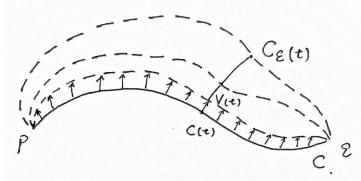
\includegraphics[width=0.2\textwidth]{fig/bo_d4vqblv7aajc73ft760g_25_1348_505_361_181_0.jpg}
\end{center}
\hspace*{3em} 

Figure 13. \({c}_{\epsilon }\left( t\right)\) , varieties of a curve \(c\) , and the corresponding "tangent vector" \(V\left( t\right)\)

which means we need to say what are variations of a curve.

\HRule

Definition 46 (Varieties of a curve)

\HRule

If \(c : \left\lbrack  {0,1}\right\rbrack   \rightarrow  S\) is a curve from \(p = c\left( 0\right)\) to \(q = c\left( 1\right)\) , then a smooth varieties of \(c\) is a family of curves \({c}_{\epsilon }\) , depending on some particular \(\epsilon  \in  \left\lbrack  {0,1}\right\rbrack\) such that \(\widehat{c} : \left\lbrack  {0,1}\right\rbrack   \times  \left\lbrack  {0,1}\right\rbrack   \rightarrow \; S\) is smooth, written as \(\widehat{c}\left( {t,\epsilon }\right)  = {c}_{\epsilon }\left( t\right)\) , and \({c}_{\epsilon }\) is just \(c\) , i.e. \(\widehat{c}\left( {t,0}\right)  = c\left( t\right)\) . If \({c}_{\epsilon }\left( 0\right)  = p\) and \({c}_{\epsilon }\left( 1\right)  = q\) , the \({c}_{\epsilon }\) is said to be variation with fixed endpoints.

\HRule

Definition 47 ("Tangent vector")

\HRule

For a variation \({c}_{\epsilon }\) , the variational vector field \(V\left( t\right)  = {\left. \frac{\partial {c}_{\epsilon }\left( t\right) }{\partial \epsilon }\right| }_{\epsilon  = 0}\) is a vector field along c. If \({c}_{\epsilon }\) has fixed endpoints, then \(V\left( 0\right)  = 0 = V\left( 1\right)\) .

\[
E\left( c\right)  = \frac{1}{2}{\int }_{0}^{1}{\left| \dot{c}\left( \tau \right) \right| }^{2}{d\tau }
\]

\HRule

Definition 48 (The energy of curve)

\HRule

Proposition 19 If \({c}_{\epsilon }\) is a smooth variation of a regular curve \(c\) , with fixed endpoints, then

\[
{\left. \frac{d}{d\epsilon }\right| }_{0}L\left( {c}_{\epsilon }\right)  =  - {\int }_{0}^{1}\frac{I\left( {V\left( \tau \right) ,\frac{\nabla }{dt}\dot{c}\left( \tau \right) }\right) }{\left| \dot{c}\left( \tau \right) \right| }{d\tau }
\]

\[
{\left. \frac{d}{d\epsilon }\right| }_{0}E\left( {c}_{\epsilon }\right)  =  - {\int }_{0}^{1}I\left( {V\left( \tau \right) ,\frac{\nabla }{dt}\dot{c}\left( \tau \right) }\right) {d\tau }
\]

where \(V\left( t\right)\) is the variational vector field of \({c}_{\epsilon }\) .

Proof

\[
{\left. \frac{d}{d\epsilon }\right| }_{0}E\left( {c}_{\epsilon }\right)  = {\left. \frac{1}{2}{\int }_{0}^{1}\frac{\partial }{\partial \epsilon }\right| }_{\epsilon  = 0}{\left| \dot{c}\left( \tau \right) \right| }^{2}{d\tau }
\]

\[
= \frac{1}{2}{\int }_{0}^{1}I\left( {{\left. \frac{\nabla }{d\epsilon }\right| }_{\epsilon  = 0}{\dot{c}}_{\epsilon }\left( \tau \right) ,\dot{c}\left( \tau \right) }\right)  + I\left( {{\left. \dot{c}\left( \tau \right) ,\frac{\nabla }{d\epsilon }\right| }_{\epsilon  = 0}{\dot{c}}_{\epsilon }\left( \tau \right) }\right) {d\tau }
\]

\[
= {\int }_{0}^{1}I\left( {{\left. \frac{\nabla }{d\epsilon }\right| }_{\epsilon  = 0}{\dot{c}}_{\epsilon }\left( \tau \right) ,\dot{c}\left( \tau \right) }\right) {d\tau }
\]

\[
= {\int }_{0}^{1}I\left( {{\left. \frac{\nabla }{d\epsilon }\right| }_{\epsilon  = 0}{\left. \frac{d}{dt}\right| }_{t = \tau }{c}_{\epsilon }\left( t\right) ,\dot{c}\left( \tau \right) }\right) {d\tau }
\]

\[
= {\int }_{0}^{1}I\left( {{\left. \frac{\nabla }{dt}\right| }_{t = \tau }V\left( t\right) ,\dot{c}\left( \tau \right) }\right) {d\tau }
\]

\[
= {\int }_{0}^{1}{\left. \frac{d}{dt}\right| }_{t = \tau }I\left( {V\left( t\right) ,\dot{c}\left( t\right) }\right)  - I\left( {V\left( \tau \right) ,{\left. \frac{\nabla }{dt}\right| }_{t = \tau }\dot{c}\left( t\right) }\right) {d\tau }
\]

\[
= I\left( {V\left( 1\right) ,\dot{c}\left( 1\right) }\right)  - I\left( {V\left( 0\right) ,\dot{c}\left( 0\right) }\right)  - {\int }_{0}^{1}I\left( {V\left( \tau \right) ,{\left. \frac{\nabla }{dt}\right| }_{t = \tau }\dot{c}\left( t\right) }\right) {d\tau }
\]

\[
=  - {\int }_{0}^{1}I\left( {V\left( \tau \right) ,{\left. \frac{\nabla }{dt}\right| }_{t = \tau }\dot{c}\left( t\right) }\right) {d\tau }
\]

Proof for \(L\) is exactly the same.

Regularity of \(c\) is only needed for the varieties of \(L\) , not of \(E\) . Problems like this are usually the reason why the energy is slightly better behaved than then length.

Theorem 17

Let \(c\) be a curve in \(S\) with constant speed, then \(c\) is a geodesic if and only if it is an extreme of the energy and length functional. That is

\[
{\left. \frac{d}{d\epsilon }\right| }_{0}E\left( {c}_{\epsilon }\right)  = 0 = {\left. \frac{d}{d\epsilon }\right| }_{0}L\left( {c}_{\epsilon }\right)
\]

for any smooth variation \({c}_{\epsilon }\) with fixed endpoints.

Proof

\(\Rightarrow\) clear from previous proposition, since \(\frac{\nabla }{dt}\dot{c} = 0\) for a geodesic.

\(\Leftarrow\) If \(\frac{\nabla }{dt}\dot{c} \neq  0\) , then there exists a variaties \({c}_{\epsilon }\) with vector field \(V = \frac{\nabla }{dt}\dot{c}\) , thus

\[
{\left. \frac{d}{d\epsilon }\right| }_{0}E\left( {c}_{\epsilon }\right)  =  - {\int }_{0}^{1}I\left( {\frac{\nabla }{dt}\dot{c},\frac{\nabla }{dt}\dot{c}}\right) {d\tau } < 0
\]

contradicts with the fact that \({\left. \frac{\mathrm{d}}{\mathrm{d}\epsilon }\right| }_{0}E\left( {c}_{\epsilon }\right)  = 0\) .

Remark

Every point \(p\) has a sufficially small neighborhood \(U\) such that there is exactly one shortest connection \(c\) from \(p\) to any \(q \in  U\) , and \(c\) is then a geodesic.

Locally, geodesics minimize the length or energy. But globally not, for example, points on the sphere can be connected by many different geodesics (great circles).

\HRule

Theorem 18 (Hopf-Rinow, metrically complete)

\HRule

Let \(S\) be a connected surface (every two points can be connected by smooth curves). Assume that every geodesic exists for all times, then for every \(q \in  S\) , there exists a

geodesic \(c\) form \(p\) to \(q\) such that

\[
d\left( {p,q}\right)  = L\left( c\right)
\]

But the geodesic doesn’t exist for all times. And whatever curve \(c\) from \(p \rightarrow  q\) has

\[
L\left( c\right)  > d\left( {p,q}\right)
\]

Similar to the uniqueness and existence theorem for parallel transport, we can show that there is a unique geodesic starting at a given point in a given direction.

For \(p \in  S\) , the exponential map

\[
{\exp }_{p} : {\mathrm{T}}_{p}S \supseteq  {V}_{p} \rightarrow  S
\]

is given by \({\exp }_{p}\left( V\right)  = {c}_{V}\left( 1\right)\) , where \({c}_{V}\) is the geodesic with \(c\left( 0\right)  = p,\dot{c}\left( 0\right)  = V\) , and \({V}_{p}\) contains all \(V \in  {\mathrm{T}}_{p}S\) for which \({c}_{V}\) is defined at least up to time \(t = 1\) .

Remark - Then \({\exp }_{p}\left( {tV}\right)  = {c}_{V}\left( t\right)\) for all \(t \in  \left\lbrack  {0,1}\right\rbrack\) (by uniqueness of geodesics).

\begin{itemize}\relax
\item\relax \({\exp }_{p}\) collects all geodesics starting at \(p\) .
\end{itemize}

\begin{itemize}\relax
\item\relax For small enough \({V}_{p},{\exp }_{p}\) is diffeomorphism of \({V}_{p}\) onto a neighborhood of \(p\) in \(S\) .
\end{itemize}

Get polar coordinates as follows

\begin{itemize}\relax
\item\relax Choose an orthonormal basis \({f}_{1}\) and \({f}_{2}\) in \({\mathrm{T}}_{p}S\) , then
\end{itemize}

\[
V = r\cos \varphi {f}_{1} + r\sin \varphi {f}_{2}
\]

for all nonzero \(v \in  {\mathrm{T}}_{p}S,r > 0,\varphi  \in  \lbrack 0,{2\pi })\) .

\begin{itemize}\relax
\item\relax Transport it via the exp map
\end{itemize}

\[
{\phi }_{p}\left( {r,\varphi }\right)  = {\exp }_{p}\left( {r\cos \varphi {f}_{1} + r\sin \varphi {f}_{2}}\right)
\]

which is well-defined if \(r\) is small enough, and is called the geodesic polar mapping at \(p\) .

\begin{itemize}\relax
\item\relax Pushforward of tangent space:
\end{itemize}

\[
\frac{\partial }{\partial r}\left( q\right)  = {T}_{\left( r,\varphi \right) }{\phi }_{p}\left( {\frac{\partial }{\partial r}\left( {r,\varphi }\right) }\right)
\]

\[
\frac{\partial }{\partial \varphi }\left( q\right)  = {T}_{\left( r,\varphi \right) }{\phi }_{p}\left( {\frac{\partial }{\partial \varphi }\left( {r,\varphi }\right) }\right)
\]

where \(q = {\phi }_{p}\left( {r,\varphi }\right)\) , and we have

\({I}_{q}\left( {\frac{\partial }{\partial r},\frac{\partial }{\partial r}}\right)  = 1\;\) radial geodesics have unit speed \({I}_{q}\left( {\frac{\partial }{\partial r},\frac{\partial }{\partial \varphi }}\right)  = 0\;\) radial geod \(\bot\) polar circle

\[
{I}_{q}\left( {\frac{\partial }{\partial \varphi },\frac{\partial }{\partial \varphi }}\right)  > 0
\]

\begin{center}
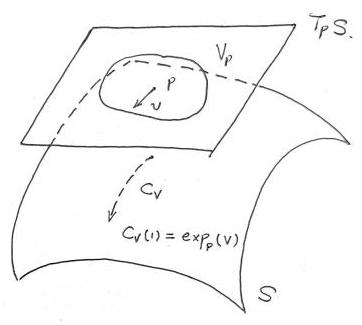
\includegraphics[width=0.2\textwidth]{fig/bo_d4vqblv7aajc73ft760g_27_1350_573_362_325_0.jpg}
\end{center}
\hspace*{3em} 

Figure 14. Exponential map

\HRule

\begin{center}
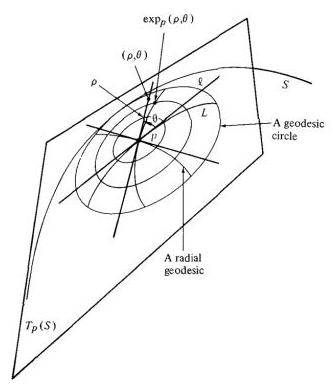
\includegraphics[width=0.2\textwidth]{fig/bo_d4vqblv7aajc73ft760g_27_1365_1187_333_389_0.jpg}
\end{center}
\hspace*{3em} 

Figure 15. Polar coordinates

Definition 49

(Exponential map)

Definition 50 (Coordinates via geodesics)

\HRule

The representation of \(I\) with respect to \({\psi }_{p}\) is

\[
{\phi }_{p}^{ * }I = \left( \begin{matrix} 1 & 0 \\  0 & G\left( {r,\varphi }\right)  \end{matrix}\right)  = \left( \begin{matrix} 1 & 0 \\  0 & {I}_{{\phi }_{p}\left( {r,\varphi }\right) }\left( {\frac{\partial }{\partial \varphi },\frac{\partial }{\partial \varphi }}\right)  \end{matrix}\right)
\]

The distance between \({\phi }_{p}\left( {r,\varphi }\right)\) and \({\phi }_{p}\left( {r,\varphi  + \epsilon }\right)\) is approx

\[
\epsilon \left| \frac{\partial {\phi }_{p}\left( {r,\varphi }\right) }{\partial \varphi }\right|  = \epsilon \sqrt{{I}_{{\phi }_{p}\left( {r,\varphi }\right) }\left( {\frac{\partial }{\partial \varphi },\frac{\partial }{\partial \varphi }}\right) } = \epsilon \sqrt{G\left( {r,\varphi }\right) }
\]

\begin{center}
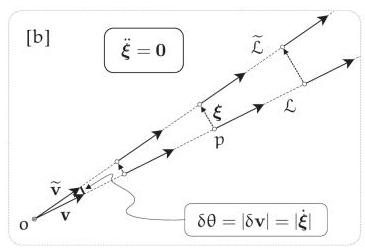
\includegraphics[width=0.2\textwidth]{fig/bo_d4vqblv7aajc73ft760g_28_1347_490_365_249_0.jpg}
\end{center}
\hspace*{3em} 

Figure 16. In the plane, even though these geodesics diverge from each other, they do so without any force pushing them apart, their relative acceleration vanishes.

Therefore, if \(\frac{\partial }{\partial }\sqrt{G} > 0\) , the distance between geodesics is increasing with larger \(r\) , and thus radial geodesics are spreading apart.

Example

ple In the plane \({\mathbb{R}}^{2}\) , with standard coordinate, \(G\left( {r,\varphi }\right)  = {r}^{2},\frac{\partial }{\partial r}\sqrt{G} = 1,\frac{{\partial }^{2}}{{\partial }^{2}r}\sqrt{G} = 0\) .

Theorem 19 \(\sqrt{G}\) satisfies the Jacobi diff eq

\[
\frac{{\partial }^{2}}{\partial {r}^{2}}\sqrt{G} + \kappa \left( p\right) \sqrt{G} = 0
\]

which means neighbouring geodesics travelling through a region of negative curvature are repelled by each other, accelerating apart. And \(\sqrt{G}\) has Taylor ex

\[
\sqrt{G}\left( {r,\varphi }\right)  = r + \frac{1}{2}\frac{{\partial }^{2}\sqrt{G}}{\partial {r}^{2}}{r}^{2} + \frac{1}{6}\frac{{\partial }^{3}\sqrt{G}}{\partial {r}^{3}}{r}^{3} + \mathcal{O}\left( {r}^{4}\right)
\]

\[
= r + \frac{1}{2}\left( {-\kappa \left( p\right) \sqrt{G}}\right) {r}^{2} + \frac{1}{6}\frac{\partial \left( {-\kappa \left( p\right) \sqrt{G}}\right) }{\partial r}{r}^{3} + \mathcal{O}\left( {r}^{4}\right)
\]

\[
= r - \kappa \left( p\right) \frac{{r}^{3}}{6} + \mathcal{O}\left( {r}^{4}\right) ,\;p = {\phi }_{p}\left( {0,\varphi }\right) ,\;r \geq  0
\]

Remark

\begin{itemize}\relax
\item\relax The role of speeding of the radial geodesics depends only on Gaussian Curvature. For \(\kappa  > 0\) , the speeding is slower than on \({\mathbb{R}}^{2}\) . This gives another way to measure \(\kappa\) intrinsically, i.e. gives another proof of Gaussian theorem.
\end{itemize}

\begin{itemize}\relax
\item\relax Go some fixed distance \(R\) away from a point \(p\) along a geodesic, this gives the polar circle \({C}_{R}\)
\end{itemize}

\[
{C}_{R}\left( \varphi \right)  = {\phi }_{p}\left( {R,\varphi }\right)
\]

\begin{itemize}\relax
\item\relax measure the length of \({C}_{R}\) :
\end{itemize}

\[
L\left( {C}_{R}\right)  = {\int }_{0}^{2\pi }\sqrt{I\left( {\frac{\partial }{\partial \varphi },\frac{\partial }{\partial \varphi }}\right) }{d\varphi } = {\int }_{0}^{2\pi }\sqrt{G\left( {R,\varphi }\right) }{d\varphi }
\]

\[
\approx  {2\pi }\left( {R - \kappa \left( p\right) \frac{{R}^{3}}{6} + \mathcal{O}\left( {R}^{3}\right) }\right)
\]

\[
= {2\pi R} - \frac{\pi }{3}{R}^{3}\kappa \left( p\right)  + \mathcal{O}\left( {R}^{3}\right)
\]

Transfer, get

\[
\kappa \left( p\right)  = \mathop{\lim }\limits_{{R \rightarrow  0}}\frac{3}{\pi } \cdot  \frac{{2\pi R} - L\left( {C}_{R}\right) }{{R}^{3}}
\]

Section 14

Fundamental theorem for surfaces

For curves, we reconstruct the curve from curvature and torsion, with \(\parallel \dot{c}\parallel  = 1\) ; for surfaces, we construct the surface from

\begin{itemize}\relax
\item\relax Gaussian curvature is not enough, as plane and the cylinder both have \(\kappa  = 0\) .
\end{itemize}

\begin{itemize}\relax
\item\relax The first fundamental form doesn't say anything about the normal.
\end{itemize}

\begin{itemize}\relax
\item\relax The first and second fundamental forms.
\end{itemize}

The problem is, \(I\) and \({II}\) are forms on \({\mathrm{T}}_{p}S\) , which means we need to have \(S\) first to specify \(I\) and \({II}\) . But we hope to reconstruct a local map of a surface from the local map of \(I\) and \({II}\) .

If \(S\) is a parameterized surface via \(\psi  : {\mathbb{R}}^{2} \supseteq  D \rightarrow  S\) , then

\[
g = \left( \begin{array}{ll} {g}_{11} & {g}_{12} \\  {g}_{21} & {g}_{22} \end{array}\right)  = {\psi }^{ * }I,\;l = \left( \begin{array}{ll} {l}_{11} & {l}_{12} \\  {l}_{21} & {l}_{22} \end{array}\right)  = {\psi }^{ * }{II}
\]

where \(g\) and is the families of symmetric metrics, parameterized by points \(\left( {x,y}\right)  \in  D\) .

Given two matrices \(g\) and \(l\) (parameterized by \(D\) ), can we construct \(\psi  : D \rightarrow  {\mathbb{R}}^{2}\) with first and second form \(I\) and \({II}\) on \(\psi \left( D\right)  = S\) such that \({\psi }^{ * }I = g\) and \({\psi }^{ * }{II} = l\) ? To find the map \(\psi\) , here we first let \({\psi }^{ * }{e}_{1},{\psi }^{ * }{e}_{2}\) be an orthonormal frame on \(D \subseteq  {\mathbb{R}}^{2}\) with respect to \(g\) , using Schmidt orthogonalization:

\[
{\psi }^{ * }{e}_{1} = \frac{1}{\sqrt{{g}_{11}}}\partial x,\;{\psi }^{ * }{e}_{2} = \sqrt{\frac{{g}_{11}}{{g}_{11}{g}_{22} - {g}_{12}^{2}}}\left( {-\frac{{g}_{12}}{{g}_{11}}\partial x + \partial y}\right)
\]

then we can get the dual frame \({\psi }^{ * }{\theta }^{1},{\psi }^{ * }{\theta }^{2}\) . After that, using 1st structure equations:

\[
d\left( {{\psi }^{ * }{\theta }^{1}}\right)  = \left( {{\psi }^{ * }{\omega }_{1}^{2}}\right)  \land  \left( {{\psi }^{ * }{\theta }^{2}}\right)
\]

\[
d\left( {{\psi }^{ * }{\theta }^{2}}\right)  = \left( {{\psi }^{ * }{\omega }_{2}^{1}}\right)  \land  \left( {{\psi }^{ * }{\theta }^{1}}\right)
\]

\HRule

Definition 51 (Pullback of \(I\) and II form)

\HRule

we can calculate \({\psi }^{ * }{\omega }_{1}^{2}\) . Next we need to calculate \({\psi }^{ * }{\omega }_{1}^{3}\) :

\[
{\psi }^{ * }{\omega }_{1}^{3} = \left( {{\psi }^{ * }{\omega }_{1}^{3}}\right) \left( {\partial x}\right) {dx} + \left( {{\psi }^{ * }{\omega }_{1}^{3}}\right) \left( {\partial y}\right) {dy}
\]

\[
= {\omega }_{1}^{3}\left( {{\mathrm{\;T}}_{p}\psi \left( {\partial x}\right) }\right) {dx} + {\omega }_{1}^{3}\left( {{\mathrm{\;T}}_{p}\psi \left( {\partial y}\right) }\right) {dy}
\]

\[
= {\omega }_{1}^{3}\left( { < {\mathrm{T}}_{p}\psi \left( {\partial x}\right) ,{e}_{1} > {e}_{1} +  < {\mathrm{T}}_{p}\psi \left( {\partial x}\right) ,{e}_{2} > {e}_{2}}\right) {dx} +
\]

\[
{\omega }_{1}^{3}\left( { < {\mathrm{T}}_{p}\psi \left( {\partial y}\right) ,{e}_{1} > {e}_{1} +  < {\mathrm{T}}_{p}\psi \left( {\partial y}\right) ,{e}_{2} > {e}_{2}}\right) {dy}
\]

\[
= \left( {{l}_{11} < {\mathrm{T}}_{p}\psi \left( {\partial x}\right) ,{e}_{1} >  + {l}_{21} < {\mathrm{T}}_{p}\psi \left( {\partial x}\right) ,{e}_{2} > }\right) {dx} +
\]

\[
\left( {{l}_{11} < {\mathrm{T}}_{p}\psi \left( {\partial y}\right) ,{e}_{1} >  + {l}_{21} < {\mathrm{T}}_{p}\psi \left( {\partial y}\right) ,{e}_{2} > }\right) {dy}
\]

\[
= \left( {{l}_{11} < {dx},{\psi }^{ * }{e}_{1} >  + {l}_{21} < {dx},{\psi }^{ * }{e}_{2} > }\right) {dx} +
\]

\[
\left( {{l}_{11} < {dy},{\psi }^{ * }{e}_{1} >  + {l}_{21} < {dy},{\psi }^{ * }{e}_{2} > }\right) {dy}
\]

\[
= \mathop{\sum }\limits_{{i = 1,2}}{l}_{i1}\left( { < d{x}^{1},{\psi }^{ * }{e}_{i} >  +  < d{x}^{2},{\psi }^{ * }{e}_{i} > }\right) d{x}^{i}
\]

\[
= \mathop{\sum }\limits_{{i,j = 1,2}}{l}_{i1} < d{x}^{j},{\psi }^{ * }{e}_{i} > d{x}^{i}
\]

\({\psi }^{ * }{\omega }_{2}^{3}\) is similar.

\[
d{\omega }_{1}^{2} = 0
\]

\[
d{\omega }_{1}^{3} = 0 = d{\omega }_{2}^{3}
\]

\HRule

Theorem 20 (Gauss-Godozzi equation)

\HRule

Lemma 10

Assume \({\omega }_{i}^{j}\) satisfy the Gauss-Godozzi equation, then for \({p}_{0} \in  {\mathbb{R}}^{3}\) and frame \({f}_{1},{f}_{2},{f}_{3}\) that are orthonormal basis of \({\mathbb{R}}^{2}\) , there exists a unique smooth \(\psi  : {\mathbb{R}}^{2} \supseteq  D \rightarrow  {\mathbb{R}}^{3}\) and smooth function \({e}_{1},{e}_{2},{e}_{3} : {\mathbb{R}}^{2} \supseteq  D \rightarrow  {\mathbb{R}}^{3}\) forming an orthonormal basis of \({\mathbb{R}}^{3}\) for each \(p \in  D\) such that

\[
{T}_{\left( x,y\right) }\psi \left( v\right)  = {\theta }_{\left( x,y\right) }^{1}\left( v\right) {e}_{1}\left( {x,y}\right)  + {\theta }_{\left( x,y\right) }^{2}\left( v\right) {e}_{2}\left( {x,y}\right)
\]

\[
{T}_{\left( x,y\right) }{e}_{1}\left( v\right)  = \mathop{\sum }\limits_{j}{\left( {\omega }_{i}^{j}\right) }_{\left( x,y\right) }\left( v\right) {e}_{j}\left( {x,y}\right)
\]

\[
\psi \left( 0\right)  = {p}_{0},\;{e}_{i}\left( 0\right)  = {f}_{i}
\]

Finally, we just need to solve the ODE to get the analytical expression of \({e}_{1},{e}_{2},{e}_{3}\) :

\[
d\left( \begin{array}{l} {e}_{1} \\  {e}_{2} \\  {e}_{3} \end{array}\right)  = \left( \begin{matrix} 0 & {\psi }^{ * }{\omega }_{1}^{2} & {\psi }^{ * }{\omega }_{1}^{3} \\   - {\psi }^{ * }{\omega }_{1}^{2} & 0 & {\psi }^{ * }{\omega }_{2}^{3} \\   - {\psi }^{ * }{\omega }_{1}^{3} &  - {\psi }^{ * }{\omega }_{2}^{3} & 0 \end{matrix}\right) \left( \begin{array}{l} {e}_{1} \\  {e}_{2} \\  {e}_{3} \end{array}\right)
\]

Example Assume

\[
g = \left( \begin{matrix} {a}^{2} + 1 & 0 \\  0 & {a}^{2}{x}^{2} \end{matrix}\right) ,\;l = \frac{ax}{\sqrt{{a}^{2} + 1}}\left( \begin{array}{ll} 0 & 0 \\  0 & 1 \end{array}\right)
\]

and \(D = \left\{  {\left( {x,y}\right)  \in  {\mathbb{R}}^{2} : x > 0,y \in  \left( {0,{2\pi }}\right) }\right\}\) , then

\[
{\psi }^{ * }{e}_{1} = \frac{1}{\sqrt{{a}^{2} + 1}}\partial x,\;{\psi }^{ * }{e}_{2} = \frac{1}{ax}\partial y
\]

\[
{\psi }^{ * }{\theta }^{1} = \sqrt{{a}^{2} + 1}{dx},\;{\psi }^{ * }{\theta }^{2} = {axdy}
\]

and

\[
{\psi }^{ * }{\omega }_{1}^{2} = \frac{ady}{\sqrt{{a}^{2} + 1}},\;{\psi }^{ * }{\omega }_{1}^{3} = 0,\;{\psi }^{ * }{\omega }_{2}^{3} = \frac{dy}{\sqrt{{a}^{2} + 1}}
\]

The results satisfy the Gauss-Codozzi equation, then

\[
{T}_{\left( x,y\right) }\psi  = \sqrt{{a}^{2} + 1}{dx}{e}_{1} + {axdy}{e}_{2}
\]

then we need to solve the ODE

\[
d\left( \begin{array}{l} {e}_{1} \\  {e}_{2} \\  {e}_{3} \end{array}\right)  = \left( \begin{matrix} 0 & \frac{ady}{\sqrt{{a}^{2} + 1}} & 0 \\   - \frac{ady}{\sqrt{{a}^{2} + 1}} & 0 & \frac{dy}{\sqrt{{a}^{2} + 1}} \\   - 0 &  - \frac{dy}{\sqrt{{a}^{2} + 1}} & 0 \end{matrix}\right) \left( \begin{array}{l} {e}_{1} \\  {e}_{2} \\  {e}_{3} \end{array}\right)
\]

the solution is

\[
{e}_{1} = \frac{1}{\sqrt{{a}^{2} + 1}}\left( \begin{matrix} a\cos y \\  a\sin y \\  1 \end{matrix}\right) ,\;{e}_{2} = \left( \begin{matrix}  - \sin y \\  \cos y \\  0 \end{matrix}\right) ,\;{e}_{3} = \frac{1}{\sqrt{{a}^{2} + 1}}\left( \begin{matrix}  - \cos y \\   - \sin y \\  a \end{matrix}\right)
\]

therefore

\[
\psi \left( {x,y}\right)  = x\left( \begin{matrix} a\cos y \\  a\sin y \\  1 \end{matrix}\right)
\]

\HRule

Theorem 21 (Fundamental theorem for surfaces)

\HRule

If \(g\) and \(l\) are families of symmetric matrices, with \(g\) positive def, and satisfying the Gauss-Godozzi equation, then there exists a parameterized surface \(S\) such that \(g\) and \(l\) are the local representation of \(I\) and \({II}\) of \(S\) . Locally, a surface is uniquely (up to translation and rotation) defined by its first and second fundamental form.

Look at local coordinates first. Suppose \(\psi  : {\mathbb{R}}^{2} \supseteq  D \rightarrow  S\) , and we want to know what’s the area of \(\psi \left( D\right)\) . For all vectors \(\left( {{v}_{1},0}\right)\) and \(\left( {0,{v}_{2}}\right)  \in  {\mathbb{R}}^{2}\) , the line segment from \(\psi \left( {x,y}\right)\) to \(\psi \left( {x + {v}_{1},y}\right)\) is linearly approximated by \({T}_{\left( x,y\right) }\psi \left( \left( {{v}_{1},0}\right) \right)\) . And similarly, the segment \(\psi \left( {x,y}\right)  \rightarrow  \psi \left( {x,y + {v}_{2}}\right)  \approx  {T}_{\left( x,y\right) }\psi \left( \left( {0,{v}_{2}}\right) \right)\) . Here the area of \(\psi \left( R\right)\) is approximated by the area of parallel segment of \({T}_{\left( x,y\right) }\psi \left( \left( {{v}_{1},0}\right) \right)\) and \({T}_{\left( x,y\right) }\psi \left( \left( {0,{v}_{2}}\right) \right)\) , i.e. the area of

\[
\psi \left( R\right)  \approx  \left| {{T}_{\left( x,y\right) }\psi \left( \left( {{v}_{1},0}\right) \right)  \times  {T}_{\left( x,y\right) }\psi \left( \left( {0,{v}_{2}}\right) \right) }\right|
\]

\begin{center}
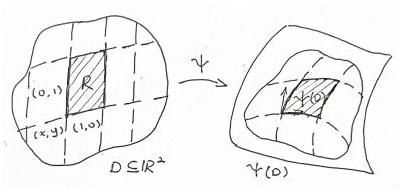
\includegraphics[width=0.3\textwidth]{fig/bo_d4vqblv7aajc73ft760g_31_1349_1555_401_191_0.jpg}
\end{center}
\hspace*{3em} 

Figure 17. Exponential map

Then, if we have a two form \({dA}\) on \(S\) satisfying

\[
{\left( dA\right) }_{p}\left( {{u}_{1},{u}_{2}}\right)  = \left| {{u}_{1} \times  {u}_{2}}\right| ,\;\forall p \in  S
\]

thus

\[
\text{ area of }\psi \left( R\right)  \approx  {\left( {\psi }^{ * }\left( dA\right) \right) }_{\left( x,y\right) }\left( {\left( {{v}_{1},0}\right) ,\left( {0,{v}_{2}}\right) }\right)
\]

\[
= {\left( dA\right) }_{\psi \left( {x,y}\right) }\left( {{T}_{\left( x,y\right) }\psi \left( \left( {{v}_{1},0}\right) \right) ,{T}_{\left( x,y\right) }\psi \left( \left( {0,{v}_{2}}\right) \right) }\right)
\]

And we have

\[
\text{ area of }\psi \left( D\right)  = \mathop{\sum }\limits_{R}\text{ area of }\psi \left( R\right)  = \mathop{\sum }\limits_{R}{dA}\left( {{T\psi }\left( \left( {1,0}\right) \right) ,{T\psi }\left( \left( {0,1}\right) \right) }\right)
\]

\[
= {\int }_{D}{\psi }^{ * }{dA} = {\int }_{\psi \left( D\right) }{dA}
\]

However, integration needs an orientation, and with the wrong orientations, we may get a negative area, which means we need to incorporate the normal in the def of \({dA}\) .

\HRule

Definition 52 (Area element and Total area)

\HRule

Let \(S\) be a surface, oriented by a unit speed field \(n\) . The area element is the 2 -form \({dA}\) on \(S\) defined by

\[
{\left( dA\right) }_{p}\left( {{u}_{1},{u}_{2}}\right)  = {n}_{p} \cdot  \left( {{u}_{1} \times  {u}_{2}}\right)
\]

The total area of \(S\) is defined by

\[
{\int }_{S}{dA}
\]

Example - On the plane \({\mathbb{R}}^{2},{dA} = {dx} \land  {dy}\)

\begin{itemize}\relax
\item\relax On the unit sphere, \({\left( dA\right) }_{p}\left( {{u}_{1},{u}_{2}}\right)  = {n}_{p} \cdot  \left( {{u}_{1} \times  {u}_{2}}\right)\) and according to one of the total area
\end{itemize}

\[
{\int }_{{S}^{2}}{dA} = {4\pi }
\]

\({trk}\) Be careful! The notation \({dA}\) is misleading as it suggests that there is a 1-form \(A\) on \(S\) such that the area element is \({dA}\) , i.e. exterior diff of \(A\) . For example, it may be misread from \({dA} = {dx} \land  {dy} = d\left( {xdy}\right)\) that \(A = {xdy}\) . Normally, \({dA}\) is not exact. If so, then by stokes theorem, we have

\[
{\int }_{S}{dA} = {\int }_{\partial S}A = 0
\]

for every compact surface without boundary.

Proposition 20 For every frame \({e}_{1},{e}_{2},{e}_{3}\) adapted to \(S\) , with dual frame \({\theta }^{1},{\theta }^{2},{\theta }^{3}\) , we have

\[
{dA} =  \pm  {\theta }^{1} \land  {\theta }^{2}
\]

Proof enough to verify this formula when evaluated on \({e}_{1}\) and \({e}_{2}\) :

\[
{\left( dA\right) }_{p}\left( {{e}_{1}\left( p\right) ,{e}_{2}\left( p\right) }\right)  = {e}_{3}\left( p\right)  \cdot  \left( {{e}_{1}\left( p\right)  \times  {e}_{2}\left( p\right) }\right)  =  \pm  1
\]

\[
{\left( {\theta }^{1} \land  {\theta }^{2}\right) }_{p}\left( {{e}_{1}\left( p\right) ,{e}_{2}\left( p\right) }\right)  = {\theta }_{p}^{1}\left( {{e}_{1}\left( p\right) }\right) {\theta }_{p}^{2}\left( {{e}_{2}\left( p\right) }\right)  - 0 = 1
\]

Section 15

Gauss-Bonnet theorem

\HRule

Theorem 22 (Gauss-Bonnet theorem)

\HRule

\(S\) compact

\[
\frac{1}{2\pi }{\int }_{S}{\kappa dA} = 2 \cdot  \left( {1 - \# \text{ holes in }S}\right)
\]

the surprising thing is the left is the local information, which is easy to measure, while the right is the global information, which is hard to measure intrinsically. Also,

the theorem tells us the holes will not change under deformations, which is called a topological invariant.

Example

\({S}_{{R}^{2}}\) has \(\kappa  = \frac{1}{{R}^{2}}\) , then

\[
\frac{1}{{2\pi }{R}^{2}}{\int }_{{S}_{{R}^{2}}}{\kappa dA} = \frac{1}{{2\pi }{R}^{2}} \cdot  {4\pi }{R}^{2} = 2
\]

There are some strange things about this theorem. For \(\int {\kappa dA}\) , we’re not clear why this should be an integer. Also, \(\kappa\) depends on the first fundamental form, but holes can just be seen and counted.

Far reaching generalizations, we guess

\(\int \{\) local data, geometric, def via some auxiliary data \(\}  =\)

Topological invariant, with some integrity, doesn't depend on the auxiliary data

Let \({e}_{1},{e}_{2},{e}_{3}\) be a frame adapted to \(S\) with dual frame \(\theta\) , positively oriented, then

\[
{\kappa dA} = \kappa {\theta }^{1} \land  {\theta }^{2} = d{\omega }_{2}^{1}
\]

Assume \(B\) is a region with \(\partial B\) smooth, then

\[
{\int }_{B}{\kappa dA} = {\int }_{B}d{\omega }_{2}^{1} = {\int }_{\partial B}{\omega }_{2}^{1} \tag{15.1}
\]

which is valid for all \(B \subseteq  S\) that have a global frame. If watch this in line integral, suppose \(c\) is a unit-speed curve such that \(\dot{c} = {e}_{1}\) , then

\[
{\omega }_{2}^{1}\left( {\dot{c}\left( t\right) }\right)  =  - {\omega }_{1}^{2}\left( {\dot{c}\left( t\right) }\right)  =  - {\kappa }_{g}\left( t\right)
\]

In general, \(\dot{c}\left( t\right)  = \cos \varphi \left( t\right) {e}_{1}\left( {c\left( t\right) }\right)  + \sin \varphi \left( t\right) {e}_{2}\left( {c\left( t\right) }\right)\) , then according to the proof of the parallel transport theorem, we have

\[
{\kappa }_{g}\left( t\right)  = \dot{\varphi }\left( t\right)  + {\omega }_{1}^{2}\left( {\dot{c}\left( t\right) }\right)
\]

Integral, we have

\[
{\int }_{a}^{b}{\kappa }_{g}\left( t\right) \mathrm{d}t = \varphi \left( b\right)  - \varphi \left( a\right)  - {\int }_{c}{\omega }_{2}^{1} = \text{ Winding number } \cdot  {2\pi } - {\int }_{c}{\omega }_{2}^{1} \tag{15.2}
\]

Substitute (15.1) into (15.2), we get

\[
{\int }_{B}{\kappa dA} + {\int }_{a}^{b}{\kappa }_{g}\left( t\right) \mathrm{d}t = \text{ Winding number } \cdot  {2\pi }
\]

\HRule

Theorem 23 (Local version of Gauss-Bonnet)

\HRule

Let \(S\) be a compact oriented surface with area element \({dA}\) . For every subset \(B \subseteq  S\) admitting a global, adapted, positively oriented frame, whose bounding curve \(\partial B : \left\lbrack  {a,b}\right\rbrack   \rightarrow  S\) is smooth, simple and unit-speed, then

\[
{\int }_{B}{\kappa dA} + {\int }_{a}^{b}{\kappa }_{g}\left( t\right) \mathrm{d}t = {2\pi }
\]

\begin{center}
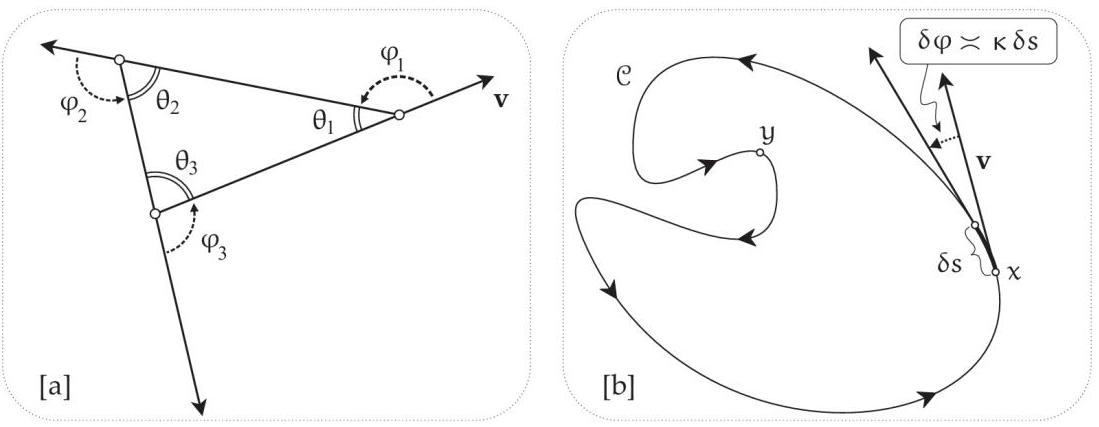
\includegraphics[width=0.8\textwidth]{fig/bo_d4vqblv7aajc73ft760g_34_212_234_1099_427_0.jpg}
\end{center}
\hspace*{3em} 

Figure 18. As a particle traces a simple loop, its velocity executes one positive revolution. In [a] \({\varphi }_{1} + {\varphi }_{2} + {\varphi }_{3} = {2\pi }\) ; in [b] \({\int }_{c}{d\varphi } =\) net rotation of \(v = {2\pi }\) .

Theorem 24 If \(\partial B\) is piece-wise smooth with interior angles \({\varphi }_{1},\cdots ,{\varphi }_{n}\) , then

\[
{\int }_{B}{\kappa dA} + {\int }_{a}^{b}{\kappa }_{g}\left( t\right) \mathrm{d}t + \left( {{n\pi } - \mathop{\sum }\limits_{i}{\varphi }_{i}}\right)  = {2\pi }
\]

particularly, in triangle, we have

\[
{\int }_{B}{\kappa dA} + {\int }_{a}^{b}{\kappa }_{g}\left( t\right) \mathrm{d}t = \mathop{\sum }\limits_{i}{\varphi }_{i} - \pi
\]

\HRule

Definition 53 (Euler characteristic)

\HRule

The Euler characteristic of a triangulation is

\[
\mathcal{X} = \# \text{ points/vertices - \#edges + \#faces }
\]

for sphere \(\mathcal{X} = 2\) , and torus \(\mathcal{X} = 0\) .

\begin{center}
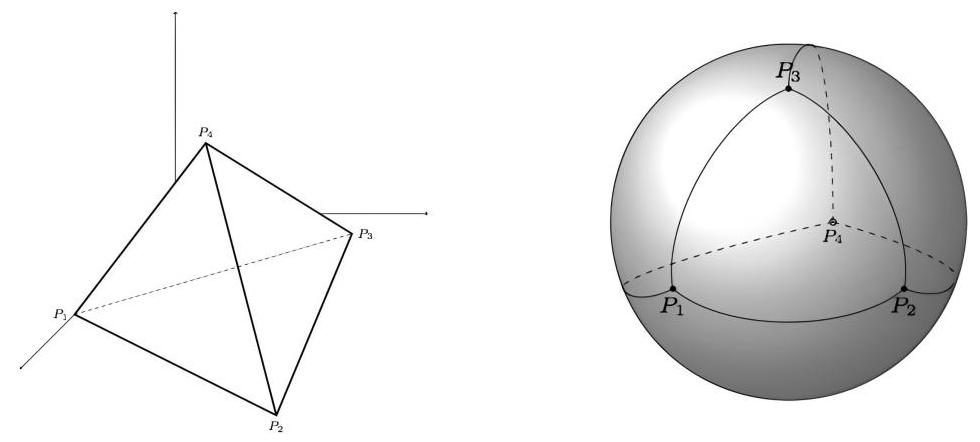
\includegraphics[width=0.7\textwidth]{fig/bo_d4vqblv7aajc73ft760g_34_246_1430_980_442_0.jpg}
\end{center}
\hspace*{3em} 

Figure 19. Since the surface of a tetrahedron is homeomorphic to the sphere \({S}^{2}\) , we may consider this as a valid triangulation for the latter. This triangulation is formed basically by four triangles, four vertices and six edges.

\begin{center}
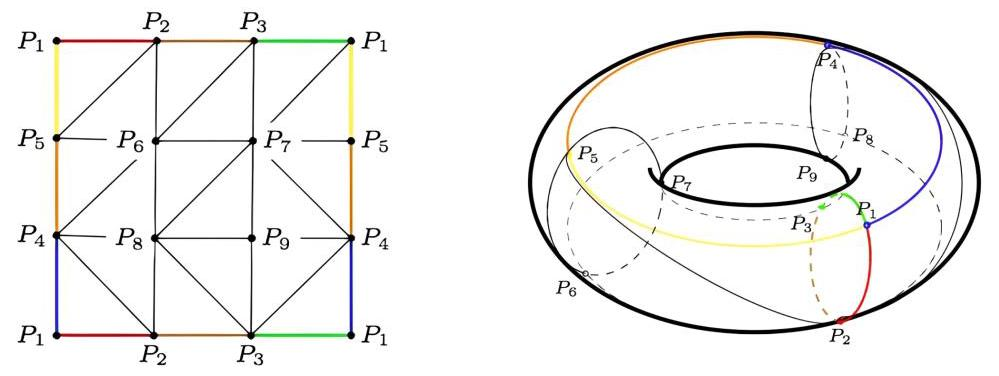
\includegraphics[width=0.7\textwidth]{fig/bo_d4vqblv7aajc73ft760g_35_280_249_999_376_0.jpg}
\end{center}
\hspace*{3em} 

Figure 20. The triangulation of a torus, performed on the representation of torus given by the quotient space of the square by the proper identification in the border.

Theorem 25

For every compact oriented surfaces \(S\) without boundary and with area element \({dA}\) and gauss curvature \(\kappa\) , we have

\[
{\int }_{S}{\kappa dA} = {2\pi }\mathcal{X}\left( S\right)
\]

this is also a version for surfaces with boundary.

Decompose \(S\) into triangles \({\Delta }_{j}\) , we can assume that the triangle is covered by a single chart, thus enabling applying local version of Gauss-Bonnet:

\[
{\int }_{S}{\kappa dA} = \mathop{\sum }\limits_{j}{\int }_{{\Delta }_{j}}{\kappa dA}
\]

\[
= \mathop{\sum }\limits_{j}\left( {{\varphi }_{1}^{j} + {\varphi }_{2}^{j} + {\varphi }_{3}^{j} - \pi  - {\int }_{\partial {\Delta }_{j}}{\kappa }_{g}}\right)
\]

Since we consider the condition without boundary, and for two triangle sharing one edge, the edge has the opposite orientation, we have

\[
\mathop{\sum }\limits_{j}{\int }_{\partial {\Delta }_{j}}{\kappa }_{g} = 0
\]

meanwhile, for a vertex, all interior angles sum up to \({2\pi }\) , i.e.

\[
\mathop{\sum }\limits_{j}\left( {{\varphi }_{1}^{j} + {\varphi }_{2}^{j} + {\varphi }_{3}^{j}}\right)  = {2\pi }
\]

therefore

\[
{\int }_{S}{\kappa dA} = {2\pi }\# \text{ vertices } - \pi \# \text{ faces }
\]

As each face has 3 edges, and each edge is shared by 2 faces, i.e. 3 \# faces = 2 \# edges, we have -\# faces = (2-3)\# faces = 2(\# faces - \# edges), thus

\[
{\int }_{S}{\kappa dA} = {2\pi }\left( {\# \text{ vertices } + \# \text{ faces } - \# \text{ edges }}\right)  = {2\pi }\mathcal{X}\left( S\right)
\]

\begin{center}
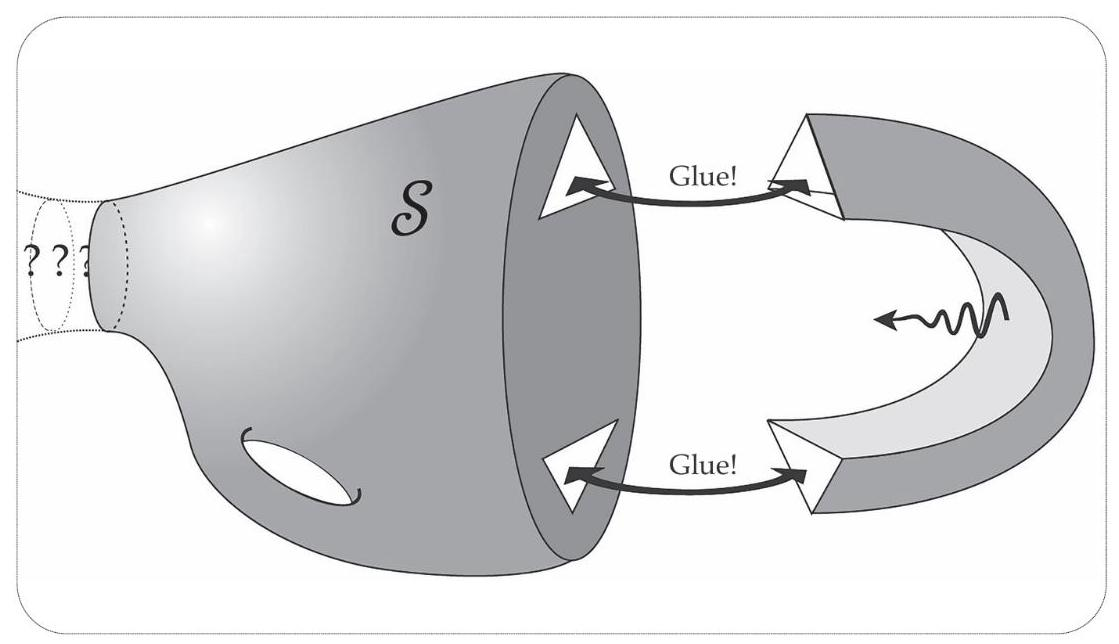
\includegraphics[width=0.8\textwidth]{fig/bo_d4vqblv7aajc73ft760g_36_195_227_1119_644_0.jpg}
\end{center}
\hspace*{3em} 

Figure 21. The general closed surface \(S\) extends to the left in an unknown manner, indicated by ???. We cut out two triangles from the triangulation (not shown) of \(S\) , reducing \(\mathcal{X}\left( S\right)\) by 2, then glue on the handle, which has no effect on \(\mathcal{X}\left( S\right)\) . Thus gluing on a handle reduces \(\mathcal{X}\left( S\right)\) by 2 .


\end{document}